\documentclass{article}

\usepackage{arxiv}          % arXiv preprint style (loads geometry + fancyhdr)

\usepackage[utf8]{inputenc}
\usepackage[T1]{fontenc}
\usepackage{lmodern}
\usepackage{amsmath,amssymb,amsthm}
\usepackage{booktabs}
\usepackage{graphicx}
\usepackage{tikz}
\usepackage{xcolor}
% Algorithm blocks are typeset with tcolorbox (the texlive 'algorithms' /
% 'algorithmicx' packages are not required and may be absent).
\usepackage[most]{tcolorbox}
\usepackage[numbers,sort&compress]{natbib}
\usepackage{url}
\usepackage[colorlinks=true,linkcolor=blue,citecolor=blue,urlcolor=blue]{hyperref}
\usepackage{cleveref}
\usepackage{placeins}

% Ruled algorithm box with a referenceable counter.
\newcounter{algctr}
\newcommand{\algcaption}[2]{\refstepcounter{algctr}\label{#2}Algorithm \thealgctr: #1}
\newtcolorbox{algo}[1]{breakable,enhanced,colback=black!3,colframe=black!55,
  fonttitle=\bfseries,coltitle=black,title={#1},boxrule=0.6pt,left=4pt,right=4pt,
  top=3pt,bottom=3pt,before upper={\small\raggedright\setlength{\parindent}{0pt}}}

% ---- Notation macros (matrices bold uppercase, vectors bold lowercase) --------
\newcommand{\M}{\mathbf{M}}
\newcommand{\Jac}{\mathbf{J}}
\newcommand{\Del}{\mathbf{D}}         % Delassus operator
\newcommand{\Ecomp}{\mathbf{E}}       % compliance
\newcommand{\Aop}{\mathbf{A}}         % regularized constraint operator
\newcommand{\Perm}{\mathbf{P}}        % permutation
\newcommand{\Lfac}{\mathbf{L}}        % unit lower-triangular LDL factor
\newcommand{\Dfac}{\mathsf{D}}         % block-diagonal LDL factor
\newcommand{\vv}{\mathbf{v}}
\newcommand{\vfree}{\mathbf{v}^{\mathrm{free}}}
\newcommand{\fext}{\mathbf{f}_{\mathrm{ext}}}
\newcommand{\blam}{\boldsymbol{\lambda}}
\newcommand{\bphi}{\boldsymbol{\phi}}
\newcommand{\rhs}{\mathbf{r}}
\newcommand{\cone}{\Upsilon}
\newcommand{\Kadm}{\mathcal{K}}          % admissible impulse cone (product)
\newcommand{\proj}{\Pi_{\cone}}
\newcommand{\projK}{\Pi_{\Kadm}}
\newcommand{\Rbb}{\mathbb{R}}
\newcommand{\uvel}{\mathbf{u}}           % constraint-space velocity
\newcommand{\gvel}{\mathbf{g}}           % dual (KKT) velocity residual
\newcommand{\stab}{\mathbf{b}}           % stabilization term
\newcommand{\reg}{\rho}                  % numerical regularization
\newcommand{\Id}{\mathbf{I}}
\newcommand{\skewm}[1]{[#1]_{\times}}    % skew-symmetric (cross-product) matrix

\theoremstyle{plain}
\newtheorem{proposition}{Proposition}
\theoremstyle{definition}
\newtheorem{remark}{Remark}

% -----------------------------------------------------------------------------
\title{GPU-Accelerated Multibody Dynamics with Frictional Contact: A Differential Variational Inequality Solver for Robot Learning}

\renewcommand{\headeright}{Technical Report}
\renewcommand{\undertitle}{}
\renewcommand{\shorttitle}{GPU-Accelerated SCC Solver}

\author{}
\date{}

\begin{document}
\maketitle
\vspace{-14pt}

\begin{center}
  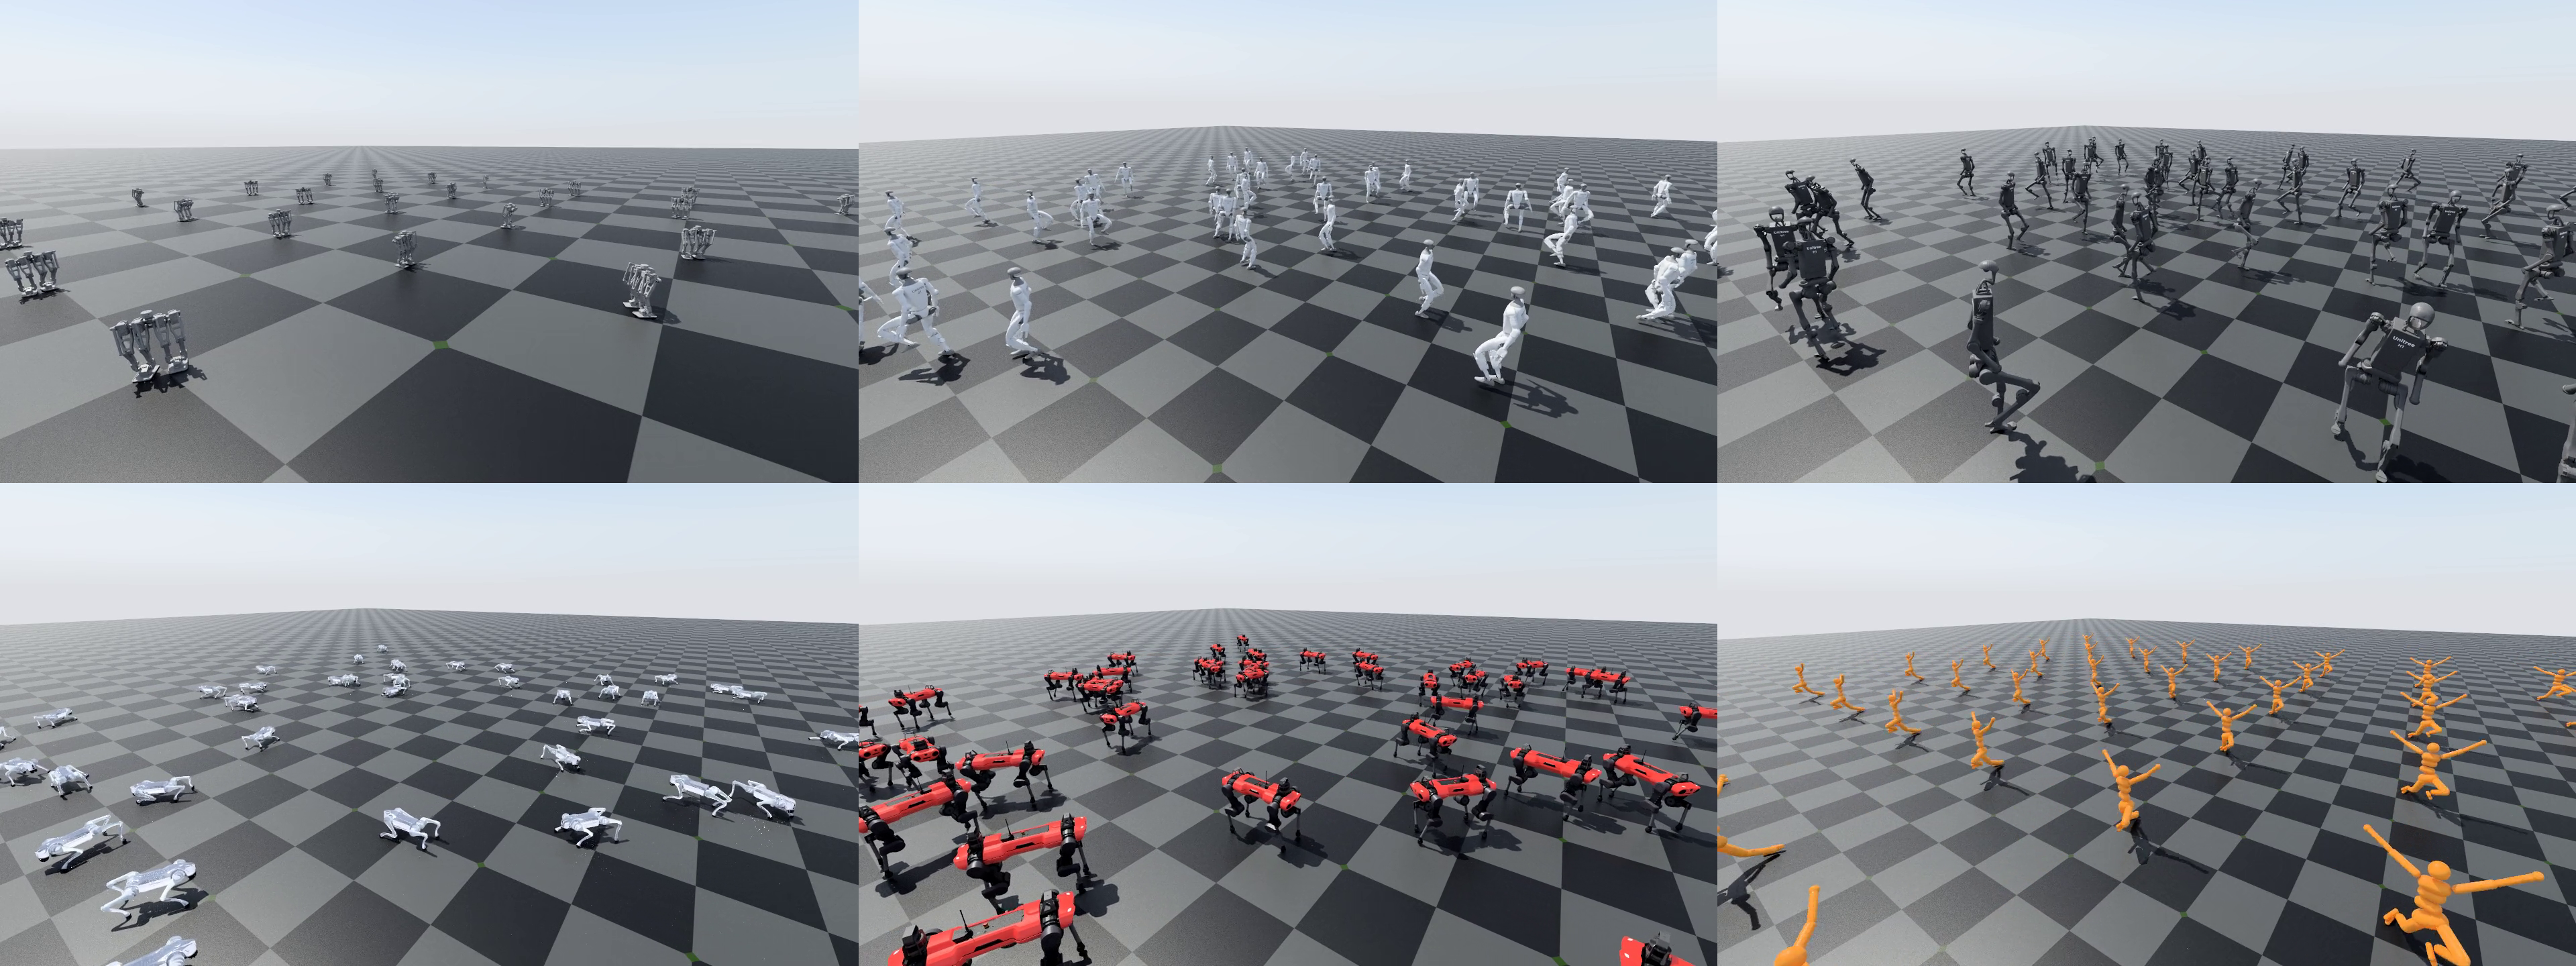
\includegraphics[width=\textwidth]{results/reinforcement_learning/figures/dvi_rl_teaser_mid.png}

  \vspace{1pt}
  {\small\textbf{Newton SCC natively supports robot learning for both
  tree-structured and closed-loop mechanisms.}}
\end{center}
\vspace{14pt}

\begin{abstract}
\mbox{}
\end{abstract}

\keywords{multibody dynamics \and frictional contact \and differential
variational inequality \and cone complementarity \and GPU simulation \and
Newton Physics Engine \and Kamino}

% =============================================================================
\section{Introduction}
\label{sec:intro}

Large batches of contact-rich simulations are now routinely used for robot
learning, controller evaluation, and synthetic-data generation
\cite{mittal2025isaaclab}. Moving this workload to a GPU does not remove its main
numerical difficulty: rigid contact is nonsmooth, and exact Coulomb friction
leads to a nonlinear, generally non-convex contact problem. A useful simulator
must therefore balance physical constraint satisfaction, convergence, and the
parallel work available in each time step. Compliant and penalty contact models
introduce stiffness--damping parameters and a contact time scale that may
constrain the time step. Hard, impulse-based contact avoids resolving a contact
spring, reducing parameter tuning and often permitting larger steps than
explicit penalty formulations; accuracy and the remaining system dynamics
still limit the time step~\cite{stewart1996,anitescu2006}.

We study this balance with a semi-implicit time-stepper in maximal coordinates.
We call the solver \emph{Split Constraint Coupling} (SCC), reflecting its
decoupled treatment of bilateral and unilateral constraints.
A differential variational inequality (DVI) couples differential
equations for state evolution with a variational inequality that selects
impulses satisfying state-dependent equality and inequality
constraints~\cite{pang2008dvi}. Here the differential equations advance
independent body states, while the variational inequality enforces joints,
limits, nonpenetration, and friction. These constraints enter as rows, so
kinematic loops are
cycles in the same constraint graph as ordinary joints. Reduced-coordinate
methods instead eliminate the joints of a selected articulation tree and treat
graph back-edges separately~\cite{featherstone2008}. They exploit linear-time
articulated-body recursions on trees. Maximal coordinates instead retain
ordinary and loop-closing joints in one graph, giving complex linkages a uniform
representation at a direct-solve cost that depends on sparse-elimination fill.
This paper develops a GPU architecture around that trade-off:
direct sparse algebra for the persistent bilateral graph and matrix-free cone
iterations for changing unilateral constraints.

The mechanics formulation follows established nonsmooth time-stepping and
cone-complementarity theory~\cite{stewart1996,anitescu2006,tasora2011}. The
research question is narrower: how can the resulting bilateral and unilateral
subproblems be organized in a GPU implementation, and what accuracy--cost
trade-offs do its iterative methods exhibit in validation, batched simulation,
and robot learning? The method is implemented in Newton using NVIDIA
Warp~\cite{warp2022}. Newton's
Kamino implementation is a maximal-coordinate dynamics framework whose primary
solver is based on proximal ADMM; SCC has subsequently been adopted as an
optional backend in the same Newton repository~\cite{tsounis2026kamino,newton2025}. The default
SCC algorithm uses one decoupled sweep over the bilateral and unilateral
constraint families, while additional alternating block sweeps retain more of
the coupling described in \Cref{sec:coupled}.

This work makes the following contributions:
\begin{itemize}
  \item a decoupled GPU architecture that combines a block-sparse $LDL^\top$
        solve for bilateral joints with matrix-free projected Jacobi,
        accelerated projected gradient descent (APGD), and preconditioned
        spectral projected gradient with fallback (P-SPG-FB) contact
        iterations and unilateral joint-limit projections;
  \item a GPU-accelerated implementation with block-sparse joint algebra,
        matrix-free contact updates, warm starts, and CUDA-graph execution; and
  \item an experimental study combining numerical validation,
        contact-solver comparisons, batched timing,
        and end-to-end policy learning on tree-structured and closed-loop
        robots; a learned quadrupedal locomotion policy is also evaluated
        in MuJoCo-C and on physical hardware.
\end{itemize}
Where applicable, we compare with MuJoCo Warp (MJWarp), a GPU implementation of
MuJoCo dynamics~\cite{mujocowarp2026}. The comparison uses matched scenarios
and timing boundaries while retaining each implementation's coordinate
representation, contact model, and numerical method. MJWarp therefore
provides a reference point for the computational trade-off between reduced-
and maximal-coordinate simulation.

% =============================================================================
\section{Related Work}
\label{sec:related}

Implicit nonsmooth time-stepping resolves contact impulses and post-step
velocities without explicitly resolving the time of every impact
event~\cite{stewart1996,anitescu2006}.
Cone-complementarity problems (CCPs) extend this approach to frictional systems,
and matrix-free cone projections avoid assembling a dense constraint-space
operator~\cite{tasora2011}. Newton SCC follows this line of work; the convex
Coulomb relaxation used here is specified in \Cref{sec:taxonomy}.
Bullet's GPU projected Gauss--Seidel solver and PhysX's PGS/TGS solvers use
related row-local iterations~\cite{coumans2014bullet,nvidia2026physx}.

GPU parallelism favors inexpensive local contact updates, whereas the
persistent bilateral graph admits sparse direct algebra. We combine
matrix-free projected Jacobi, APGD, and P-SPG-FB contact iterations with a
block-sparse $LDL^\top$ bilateral solve whose cost depends on elimination
fill~\cite{davis2006}. APGD uses Nesterov acceleration for the cone-constrained
quadratic objective~\cite{nesterov1983,heyn2013}. P-SPG-FB combines
preconditioning, Barzilai--Borwein step selection, a nonmonotone line search,
and a fallback iterate~\cite{barzilai1988,birgin2000,heyn2013krylov,tasora2013pspgfb}.

Kamino P-ADMM solves the nonlinear frictional complementarity formulation with
globally coupled updates; SCC uses the convex Anitescu relaxation and a
decoupled bilateral--unilateral solve~\cite{tsounis2025,tsounis2026kamino}.
SCC is also available as an optional backend in Newton's Kamino
framework~\cite{newton2025}.

Coordinate representation creates the other central trade-off.
Reduced-coordinate algorithms exploit articulation trees and add closure
constraints for graph back-edges, whereas maximal coordinates retain every
joint as an explicit constraint~\cite{featherstone2008}. MuJoCo uses
reduced-coordinate dynamics with a convex contact model~\cite{todorov2014},
and MJWarp maps that formulation to GPUs~\cite{mujocowarp2026}. It serves
as the reduced-coordinate reference for the tree-structured experiments, while
DR Legs evaluates SCC's uniform treatment of ordinary joints and loop closures.

% =============================================================================
\section{Notation and Glossary}
\label{sec:notation}

Matrices are bold uppercase ($\Del,\M,\Jac$), vectors bold lowercase
($\vv,\blam,\rhs$), and scalars plain lowercase ($\alpha,\mu,h,n_c$).
Superscript $(l)$ denotes the quantity at time level $t^{(l)}$; a plus superscript
($\vv^{+}$) denotes the end-of-step value.

\begin{table}[h]
\centering
\begin{tabular}{@{}ll@{}}
\toprule
Symbol & Meaning \\
\midrule
$n_b,\ n_c$ & number of bodies and contacts \\
$m_b,\ m_\ell,\ m$ & bilateral rows, active limit rows, total constraint rows \\
$\vv,\ \vv^{+}$ & body spatial velocities at step start and end \\
$\vfree$ & predicted (unconstrained, ``free'') velocity \\
$\M,\ \M^{-1}$ & block-diagonal mass / inverse-mass operator \\
$\fext$ & external and actuation generalized forces \\
$h=\Delta t$ & time step \\
$\Jac,\ \Jac_b,\ \Jac_u$ & constraint Jacobian; bilateral and unilateral blocks \\
$\uvel=\Jac\vv$ & constraint-space velocity \\
$\blam,\ \blam_b,\ \blam_u$ & constraint impulses; bilateral and unilateral blocks \\
$\Kadm,\ \cone_i$ & product admissible set; per-contact friction cone \\
$\bphi_b,\ \bphi_u$ & joint violation; contact gap \\
$\stab$ & constraint stabilization term \\
$\Del=\Jac\M^{-1}\Jac^{\top}$ & Delassus operator \\
$\Del_{bb},\Del_{bu},\Del_{ub},\Del_{uu}$ & bilateral/unilateral blocks of $\Del$ \\
$\Ecomp,\ \reg$ & compliance matrix; numerical diagonal regularization \\
$\Aop=\Del+\Ecomp+\reg\Id$ & regularized constraint-space operator \\
$\rhs,\ \rhs_b,\ \rhs_u$ & right-hand side (per constraint family) \\
$\alpha$ & Baumgarte damping parameter \\
$\mu,\ \cone_i^{*}$ & friction coefficient; dual friction cone \\
$\proj,\ \projK$ & Euclidean projection onto $\cone_i$ / onto $\Kadm$ \\
$\Perm,\ \Lfac,\ \Dfac$ & block permutation; unit lower and block-diagonal $LDL^\top$ factors \\
\bottomrule
\end{tabular}
\caption{Notation.}
\label{tab:notation}
\end{table}

% =============================================================================
\section{Background and Preliminaries}
\label{sec:background}

\subsection{Rigid-body state and equations of motion}
\label{sec:eom}
Each of the $n_b$ bodies carries an independent position $\mathbf x_i$, unit
quaternion $\boldsymbol\varepsilon_i$, and spatial velocity
$\vv_i=(\dot{\mathbf x}_i,\boldsymbol\omega_i)$ expressed in world coordinates.
The quaternion represents the rotation $\mathbf R_i$ from body to world
coordinates. Stacking the velocities gives $\vv\in\Rbb^{6n_b}$ and a
block-diagonal symmetric positive-definite mass operator with body blocks
$\M_i=\operatorname{blkdiag}(m_i\Id_3,\mathbf I_i^W)$, where
$\mathbf I_i^W=\mathbf R_i\mathbf I_i^B\mathbf R_i^\top$. The body-frame inertia
$\mathbf I_i^B$ is diagonal in principal axes and otherwise a full symmetric
tensor. Smooth Newton--Euler motion is
augmented by impulsive constraint wrenches $\Jac^{\top}\blam$. Bilateral
impulses are unrestricted, while limit and contact impulses belong to convex
cones and satisfy complementarity with the associated constraint-space
velocity $\uvel=\Jac\vv$.

\subsection{Coordinate representations and kinematic loops}
\label{sec:coordinates-loops}
Maximal coordinates keep body states independent and express every joint as
bilateral rows. A kinematic loop is therefore a cycle in the same constraint
graph and requires no spanning tree. Reduced coordinates eliminate the joints
of an articulation tree; every non-tree edge requires a closure constraint or
equivalent treatment~\cite{featherstone2008,tsounis2025}. SCC consequently uses
the same bilateral operator for ordinary joints and loop closures, whereas
reduced-coordinate methods can exploit tree recursions.

Maximal coordinates also retain constrained relative directions explicitly.
Bilateral-row compliance can model flexibility in those directions, while
paired unilateral bounds can represent clearance. \Cref{sec:compliance}
derives the compliant model and specifies its use in the experiments.

\subsection{Constraint taxonomy}
\label{sec:taxonomy}
Constraints are \emph{bilateral} (joints: holonomic equalities
$\bphi_b(\mathbf q)=\mathbf 0$, impulses of any sign) or \emph{unilateral}
(contacts and joint limits: inequalities with sign-restricted impulses). A
\emph{joint limit} is a one-sided holonomic bound: with residual distance
$\phi_\ell(\mathbf q)\ge0$ to the limit and constraint velocity
$u_\ell=(\Jac\vv)_\ell$, it enforces the Signorini-type complementarity
\begin{equation}
0\le u_\ell \ \perp\ \lambda_\ell\ge0 ,
\label{eq:limit}
\end{equation}
i.e.\ a normal-only contact with impulse $\lambda_\ell\ge0$ that acts when the
bound is reached and vanishes otherwise; \Cref{sec:jointspace} makes the row
$(\Jac\vv)_\ell$ explicit. A
contact contributes a normal row governed by the Signorini condition
$0\le u_n\perp\lambda_n\ge0$ and two tangential rows governed by Coulomb friction
with the maximum-dissipation principle: among admissible tangential impulses,
the physical impulse maximizes dissipated power. Writing a contact impulse as
$\blam_i=(\lambda_{n,i},\boldsymbol\lambda_{t,i})$, its admissible cone is
$\cone_i=\{(\lambda_n,\boldsymbol\lambda_t):\lambda_n\ge0,\
\|\boldsymbol\lambda_t\|_2\le\mu_i\lambda_n\}$, where $\mu_i$ is the sliding
friction coefficient. The model includes sliding friction but not rolling
resistance or torsional friction. The exact model places the
impulse in this second-order friction cone and, after a De Saxc\'e
velocity shift, its dual velocity in $\cone_i^{*}$. Because that shift depends
on tangential slip, the stacked system is a nonlinear, generally non-convex
complementarity problem. The Anitescu relaxation used here omits the shift and
yields a convex CCP, at the cost of artificial normal velocity during sliding
\cite{anitescu2006,tasora2011}. \Cref{app:friction_ccp} gives the contact-level
construction.

% =============================================================================
\section{Formulation}
\label{sec:formulation}

\subsection{Semi-implicit Euler step and predicted velocity}
\label{sec:euler}
Discretizing the equations of motion of \Cref{sec:eom} over a step $h$ with a
semi-implicit Euler scheme gives the momentum balance and position update
\begin{equation}
\M\bigl(\vv^{+}-\vv\bigr) = h\,\fext + \Jac^{\top}\blam,
\qquad
\mathbf q^{+} = \mathcal I_h(\mathbf q,\vv^{+}),
\label{eq:euler}
\end{equation}
where $\mathcal I_h$ denotes the configuration update below. Velocities are
integrated \emph{before} configurations (semi-implicit), so the update uses the
post-solve velocity $\vv^{+}$. Writing $\vv_i^{+}=(\dot{\mathbf x}_i^{+},
\boldsymbol\omega_i^{+})$ for body $i$ with position $\mathbf x_i$ and unit
quaternion $\boldsymbol\varepsilon_i$, the translational part is a plain Euler
update while the orientation is advanced by the exponential map so that the unit
norm is preserved exactly:
\begin{equation}
\mathbf x_i^{+} = \mathbf x_i + h\,\dot{\mathbf x}_i^{+},
\qquad
\boldsymbol\varepsilon_i^{+} =
\exp\!\Bigl(\tfrac{h}{2}\,[\,0,\ \boldsymbol\omega_i^{+}\,]\Bigr)
\otimes\boldsymbol\varepsilon_i,
\label{eq:integrate}
\end{equation}
where $\otimes$ is quaternion multiplication and $\exp$ of the pure quaternion
$[\,0,\boldsymbol\theta\,]$ is $\bigl(\cos\|\boldsymbol\theta\|,\
\tfrac{\sin\|\boldsymbol\theta\|}{\|\boldsymbol\theta\|}\,\boldsymbol\theta\bigr)$.
The increment multiplies on the left because $\boldsymbol\omega_i^+$ is
expressed in world coordinates. The collection of these per-body maps defines
$\mathcal I_h$. This
is the exact rotational update for constant $\boldsymbol\omega_i^{+}$ over the
step and avoids the norm drift of the additive approximation
$\boldsymbol\varepsilon^{+}\approx\boldsymbol\varepsilon+h\,
\dot{\boldsymbol\varepsilon}$. Defining the \emph{predicted}
(unconstrained) velocity $\vfree=\vv+h\,\M^{-1}\fext$ --- the velocity reached in
the absence of constraints --- the momentum balance becomes
\begin{equation}
\vv^{+} = \vfree + \M^{-1}\Jac^{\top}\blam .
\label{eq:free_velocity}
\end{equation}
The mass operator, Jacobians, and contact geometry are evaluated at the
pre-step state $(\mathbf q,\vv)$ and held fixed during the constraint solve.

\subsection{Joint kinematics: motion subspace, limits, and actuation}
\label{sec:jointspace}
Joint limits and actuation act along the directions left unconstrained by a
joint's bilateral rows. For a joint between parent $p$ and child $c$,
let $\Delta\vv=\vv_c-\vv_p\in\Rbb^{6}$ be the relative spatial velocity of the two
bodies evaluated at the joint anchor. The joint's \emph{motion subspace}
$\mathbf S\in\Rbb^{6\times n_f}$ collects the $n_f$ permitted relative degrees of
freedom as columns (its screw axes); the local bilateral Jacobian
$\Jac_{b,j}$ spans the reciprocal constrained directions, so
$\Jac_{b,j}\,\Delta\vv=\mathbf 0$ constrains the remaining $6-n_f$ directions.
\Cref{app:jacobians} gives the corresponding body-space Jacobian blocks. The
joint-coordinate rates are the projection of the relative velocity onto this
subspace,
\begin{equation}
\dot{\mathbf q}_{\mathrm{jnt}} = \mathbf S^{\top}\Delta\vv .
\label{eq:jointvel}
\end{equation}
For a revolute joint with world-frame unit axis $\mathbf a$, $\mathbf S=[\,\mathbf
0;\ \mathbf a\,]$ (pure rotation), so $\dot q=\mathbf a^{\top}(\boldsymbol\omega_c-
\boldsymbol\omega_p)$; for a prismatic joint $\mathbf S=[\,\mathbf a;\ \mathbf
0\,]$ and $\dot q=\mathbf a^{\top}(\dot{\mathbf x}_c-\dot{\mathbf x}_p)$.

\paragraph{Joint limits.} A limited coordinate carries a lower bound
$q\ge q^{\mathrm{lo}}$ and/or an upper bound $q\le q^{\mathrm{hi}}$. When a bound is
violated it contributes one unilateral row (the Signorini condition
\eqref{eq:limit}) whose constraint velocity is the signed joint rate
\eqref{eq:jointvel},
\begin{equation}
u_\ell = s_\ell\,\mathbf S^{\top}\Delta\vv,\quad
\phi_\ell = s_\ell\,(q-q^{\mathrm{lim}}),\qquad
s_\ell=\!\begin{cases}+1 & \text{lower bound},\\ -1 & \text{upper bound},\end{cases}
\label{eq:limitrow}
\end{equation}
so that the row of $\Jac$ is $s_\ell\mathbf S^{\top}$ acting as $-s_\ell\mathbf S^{\top}$
on the parent and $+s_\ell\mathbf S^{\top}$ on the child, and $u_\ell\ge0$ always
points away from the bound. The impulse $\lambda_\ell\ge0$ turns on only when the
bound is reached ($\phi_\ell\le0$) and the resulting wrench $s_\ell\mathbf S\lambda_\ell$
(applied with opposite sign to parent and child) is a normal-only, one-sided
version of the bilateral joint force.

\paragraph{Actuation.} Each actuated coordinate applies a scalar generalized
force $\tau$ built from a proportional--derivative law with optional feedforward,
\begin{equation}
\tau = k_e\,(q^{*}-q) - k_d\,\dot q + \tau_{\mathrm{ff}},
\label{eq:pd}
\end{equation}
with $q^{*}$ the target coordinate and $\dot q$ from \eqref{eq:jointvel} (for
revolute DOFs the error $q^{*}-q$ is wrapped to $(-\pi,\pi]$). The force is mapped
back to the bodies through the same motion subspace as the equal-and-opposite
wrench pair
\begin{equation}
\mathbf f_c \mathrel{+}= \mathbf S\,\tau,\quad \mathbf f_p \mathrel{-}= \mathbf S\,\tau,
\label{eq:act_wrench}
\end{equation}
i.e.\ a pure torque $\mathbf a\,\tau$ for a revolute DOF and a force $\mathbf a\,\tau$
(with the induced moment about the lever arm) for a prismatic DOF. Actuation thus
enters the step through $\fext$ and hence the predicted velocity
\eqref{eq:free_velocity}. For stiff gains an explicit $-k_d\dot q$ term is unstable
at practical step sizes; substituting $\dot q=\mathbf S^{\top}\Delta\vv$ and
treating the damping and the $h\,k_e$ contribution implicitly folds the effective
gain $C_{\mathrm{eff}}=k_d+h\,k_e$ along $\mathbf a$ into an augmented inverse
inertia $\widetilde{\M}^{-1}$ that replaces $\M^{-1}$ in the predicted velocity
\eqref{eq:free_velocity} (step~2 of Algorithm~\ref{alg:step}), improving
stability for stiff gains at practical step sizes.

\subsection{The per-step saddle-point (mixed) system}
\label{sec:saddle}
The constrained step couples two laws --- the impulse--momentum balance and the
constraint law --- in the two unknowns $\vv^{+}$ and $\blam$. Written together
they form the mixed (saddle-point) system
\begin{equation}
\begin{bmatrix}\M & -\Jac^{\top}\\[2pt] \Jac & \Ecomp+\reg\Id\end{bmatrix}
\begin{bmatrix}\vv^{+}\\[2pt] \blam\end{bmatrix}
=
\begin{bmatrix}\M\vfree\\[2pt] -\stab\end{bmatrix}
+
\begin{bmatrix}\mathbf 0\\[2pt] \gvel\end{bmatrix},
\qquad
\Kadm\ni\blam \ \perp\ \gvel\in\Kadm^{*},
\label{eq:saddle}
\end{equation}
or, row by row,
\begin{align}
\M\vv^{+}-\Jac^{\top}\blam &= \M\vfree, \label{eq:saddle_mom}\\
\Kadm\ni\blam \ &\perp\ \gvel=\Jac\vv^{+}+(\Ecomp+\reg\Id)\blam+\stab\in\Kadm^{*}.
\label{eq:saddle_con}
\end{align}
The first row is the momentum balance \eqref{eq:free_velocity}. The second row is
the constraint law at the velocity level: the dual constraint-space velocity
$\gvel$ is complementary to $\blam$ over the admissible cone
$\Kadm=\Rbb^{m_b}\times\Rbb_+^{m_\ell}\times
\bigl(\textstyle\prod_{i=1}^{n_c}\cone_i\bigr)\subset\Rbb^m$, with
$m=m_b+m_\ell+3n_c$. Here $m_b$ and $m_\ell$ count scalar bilateral and active
joint-limit rows. The factors are the whole space for bilateral
rows, the nonnegative orthant for active one-sided limits, and one friction
cone per contact. The vector $\gvel$ combines the constraint velocity
$\Jac\vv^{+}$, stabilization $\stab$ (\Cref{sec:rhs}), physical compliance
$\Ecomp\blam$, and a small optional numerical regularization $\reg\blam$.

The compliance matrix $\Ecomp\succeq\mathbf 0$ enters only the $(2,2)$ block.
With $\Ecomp=\mathbf0$ and $\reg=0$, bilateral rows impose
$\Jac_b\vv^{+}+\stab_b=\mathbf0$, while unilateral rows satisfy the relaxed
frictional CCP or scalar limit complementarity. Positive compliance gives a
row finite stiffness and an impulse-proportional residual velocity.
\Cref{sec:compliance} derives its diagonal entries and $\stab$ from an implicit
spring--damper model. With zero compliance, $\alpha$ controls error recovery;
numerical regularization and finite solver tolerance can still leave residuals.
The convex friction relaxation changes the friction law, independently of
normal compliance. This full-space form, with the mass matrix
explicit, is the per-step variational inequality underlying spectral
cone-complementarity solvers~\cite{tasora2011,tasora2013pspgfb}.

\subsection{Reduction to the constraint-space Delassus system}
\label{sec:schur_mass}
Solving the momentum row \eqref{eq:saddle_mom} for $\vv^+$ and substituting it
into \eqref{eq:saddle_con} eliminates the $6n_b$ body-velocity unknowns:
\begin{equation}
\gvel = \Jac\vv^{+}+(\Ecomp+\reg\Id)\blam+\stab
      = \bigl(\underbrace{\Jac\M^{-1}\Jac^{\top}}_{\Del}+\Ecomp+\reg\Id\bigr)\blam
       + \underbrace{\Jac\vfree+\stab}_{\rhs}.
\label{eq:schur_reduction}
\end{equation}
This is a Schur complement of the saddle-point matrix \eqref{eq:saddle} with
respect to the mass block $\M$. It introduces the \textbf{Delassus operator}
$\Del=\Jac\M^{-1}\Jac^{\top}\succeq\mathbf 0$ (symmetric positive semidefinite
because $\M\succ\mathbf 0$) and the right-hand side $\rhs=\Jac\vfree+\stab$,
reducing the step to the constraint-only cone-complementarity problem
\begin{equation}
\Kadm\ni\blam\ \perp\ \underbrace{(\Del+\Ecomp+\reg\Id)}_{\Aop}\,\blam+\rhs\in\Kadm^{*}.
\label{eq:ccp}
\end{equation}
The projected contact solvers apply \eqref{eq:ccp} without forming $\Del$;
the direct bilateral solver assembles only the structurally present blocks of
its bilateral restriction. The full saddle-point matrix is never assembled.
Eliminating the bilateral impulses gives the further reduction in
\Cref{sec:coupled}.

\begin{remark}[Compliance sign convention]
\label{rem:compliance_sign}
We use the added-diagonal convention $\Del+\Ecomp$, with
$\Ecomp\succeq\mathbf 0$. Literature that defines the signed compliance term
with the opposite sign may write the same physical relation as
$\Del-\Ecomp$. Numerical regularization $\reg\Id$, $\reg>0$, enters with the
same added sign. It makes $\Aop$ positive definite even when redundant
constraint rows make $\Del$ singular; nonzero compliance on only a subset of
rows does not by itself guarantee strict definiteness of the entire system.
\end{remark}

\subsection{Compliance}
\label{sec:compliance}
For constraint coordinate $i$, consider a spring--damper with stiffness $k_i$,
damping $c_i=\alpha k_i$, violation $\phi_i$, and velocity
$u_i=(\Jac\vv)_i$. Its implicit step satisfies
\begin{equation}
\lambda_i = -h\bigl(k_i\,\phi_i^{+}+c_i\,u_i^{+}\bigr),
\qquad
\phi_i^{+}=\phi_i+h\,u_i^{+}.
\label{eq:spring}
\end{equation}
Substituting $\phi_i^{+}$ and using $c_i=\alpha k_i$,
\begin{equation}
\lambda_i = -h k_i\,\phi_i - h k_i(h+\alpha)\,u_i^{+}
\quad\Longrightarrow\quad
u_i^{+} = -\underbrace{\tfrac{\phi_i}{\,h+\alpha\,}}_{b_i}
          -\underbrace{\tfrac{1}{k_i\,h\,(h+\alpha)}}_{e_i}\,\lambda_i .
\label{eq:compliant_u}
\end{equation}
Stacking \eqref{eq:compliant_u} over all rows, with $\Jac\vv^{+}$ the stacked
$u_i^{+}$, $\stab=(b_i)$, and $\Ecomp=\operatorname{diag}(e_i)$, gives the matrix
form
\begin{equation}
\Jac\vv^{+} + \Ecomp\,\blam + \stab = \mathbf 0 ,
\label{eq:compliant_matrix}
\end{equation}
which gives the equality law for bilateral rows and active scalar unilateral
rows. Frictional contact blocks retain the cone-complementarity law
\eqref{eq:saddle_con}; their dual residual need not vanish during sliding. The
spring--damper model gives both the compliance $e_i$ and stabilization $b_i$
from the same discretization. The parameter $\alpha$ controls damping and error
recovery; $k_i\to\infty$ gives $e_i\to0$ and recovers a rigid constraint.
The same model permits bilateral-joint and joint-limit compliance. The reported
experiments apply compliance to contacts for projected Jacobi, APGD, and
P-SPG-FB, and use rigid bilateral joints and joint limits
($\Ecomp_b=\Ecomp_\ell=\mathbf0$).

\subsection{Stabilization and right-hand-side assembly}
\label{sec:rhs}
For $\phi>0$ in separation and $\phi<0$ in violation, all families use
$\stab=\bphi/(h+\alpha)$ in $\rhs=\Jac\vfree+\stab$. Bilateral rows apply it
throughout; contacts use it only on the normal row, with clamping for deep
penetration, and zero on tangential rows. Limits are one-sided
(\Cref{eq:limit}). On rigid equality rows with zero regularization,
$\Jac\vv^+=-\bphi/(h+\alpha)$; $\alpha>0$ spreads drift correction over several
steps, while $\alpha=0$ applies $\bphi/h$ in one step.

\subsection{\texorpdfstring{CCP\,$\Leftrightarrow$\,QP}{CCP--QP} equivalence}
\label{sec:ccp_qp}
On bilateral rows $\Kadm$ is the whole space and \eqref{eq:ccp} reduces to a
linear system; unilateral rows retain cone constraints. Because
$\Del\succeq\mathbf0$, the regularized operator
$\Aop=\Del+\Ecomp+\reg\Id$ is positive definite whenever $\reg>0$ (or the
physical compliance removes every null direction). The CCP is then equivalent
to the strictly convex cone-constrained quadratic program (QP)
\begin{equation}
\min_{\blam\in\Kadm}\ f(\blam)
=\tfrac12\,\blam^{\top}\Aop\blam + \rhs^{\top}\blam ,
\label{eq:qp}
\end{equation}
whose gradient is $\nabla f(\blam)=\Aop\blam+\rhs$. The
first-order optimality condition of \eqref{eq:qp} is that the negative gradient
lies in the normal cone of $\Kadm$ at the minimizer,
$-\nabla f(\blam)\in N_{\Kadm}(\blam)$; for a closed convex cone this is precisely
the cone-complementarity statement
$\Kadm\ni\blam\perp\nabla f(\blam)\in\Kadm^{*}$, i.e.\ \eqref{eq:ccp}. When
$\Aop\succ\mathbf 0$ the program is strictly convex and its solution is unique.
This equivalence lets the projected first-order solvers of
\Cref{sec:solvers} target \eqref{eq:qp} while enforcing feasibility through the
cone projection.

\subsection{Bilateral/unilateral partition and the coupled system}
\label{sec:coupled}
Partition the Jacobian and impulse into bilateral and unilateral parts,
$\Jac=[\Jac_b;\,\Jac_u]$ and $\blam=[\blam_b;\,\blam_u]$. The regularized
operator inherits a $2\times2$ block structure,
\begin{equation}
\Aop=\begin{bmatrix}\Aop_{bb}&\Del_{bu}\\ \Del_{ub}&\Aop_{uu}\end{bmatrix},
\quad
\Aop_{bb}=\Jac_b\M^{-1}\Jac_b^{\top}+\Ecomp_b+\reg\Id,\ \
\Del_{bu}=\Jac_b\M^{-1}\Jac_u^{\top}=\Del_{ub}^{\top},\ \
\Aop_{uu}=\Jac_u\M^{-1}\Jac_u^{\top}+\Ecomp_u+\reg\Id,
\label{eq:partitioned-operator}
\end{equation}
where $\Del_{bu}$ can be nonzero only when bilateral and unilateral rows act on
a common body. The reduced problem \eqref{eq:ccp} then reads
\begin{equation}
\begin{bmatrix}\Aop_{bb}&\Del_{bu}\\ \Del_{ub}&\Aop_{uu}\end{bmatrix}
\begin{bmatrix}\blam_b\\ \blam_u\end{bmatrix}
+\begin{bmatrix}\rhs_b\\ \rhs_u\end{bmatrix}
=\begin{bmatrix}\mathbf 0\\ \gvel_u\end{bmatrix},
\qquad
\blam_b\ \text{free},\ \ \Kadm_u\ni\blam_u\perp\gvel_u\in\Kadm_u^{*},
\label{eq:coupled}
\end{equation}
where $\Kadm_u$ is the product of nonnegative limit cones and contact friction
cones. Bilateral rows are equalities ($\gvel_b=\mathbf 0$); unilateral rows are
cone-complementary. Eliminating the bilateral impulses,
$\blam_b=-\Aop_{bb}^{-1}(\rhs_b+\Del_{bu}\blam_u)$, gives a second Schur
complement, now with respect to $\Aop_{bb}$:
\begin{equation}
\Kadm_u\ni\blam_u\ \perp\
\bigl(\Aop_{uu}-\Del_{ub}\Aop_{bb}^{-1}\Del_{bu}\bigr)\blam_u
+\bigl(\rhs_u-\Del_{ub}\Aop_{bb}^{-1}\rhs_b\bigr)\in\Kadm_u^{*}.
\label{eq:schur}
\end{equation}
An exact application of the condensed operator would require a bilateral solve
inside each unilateral operator evaluation. The implementation instead splits
the unilateral rows into limits $\ell$ and contacts $c$, and uses the
three-family block Gauss--Seidel order: limits, bilateral joints, then contacts.
For family $f\in\{\ell,b,c\}$, the other families' current impulses enter the
conditional right-hand side
\begin{equation}
\widetilde{\rhs}_f=\rhs_f+
\sum_{g\in\{\ell,b,c\}\setminus\{f\}}\Del_{fg}\blam_g.
\label{eq:family-rhs}
\end{equation}
Each update solves with $\Aop_{ff}$ and $\widetilde{\rhs}_f$, directly for
bilateral joints and by matrix-free cone iterations for limits and contacts.
Revisiting the families retains cross-coupling without explicitly assembling
the condensed operator.

\subsection{Reduction to the decoupled solve}
\label{sec:reduction}
The default decoupled algorithm performs one sweep in the order
$\ell\to b\to c$. The bilateral solve sees the updated limit impulses, and
the contact solve sees the updated bilateral impulses. The bilateral rows are
not revisited after the final contact increment unless the optional final
bilateral correction is enabled. Within each family solve, the other families'
impulses are fixed: the unilateral iterations therefore do not include the
bilateral response $\Del_{ub}\Aop_{bb}^{-1}\Del_{bu}$ of \eqref{eq:schur}.
Additional sweeps update every family against the others' latest impulses and
can reduce this splitting error. Convergence to the coupled solution requires
the block iteration itself to converge and the inner solves to be sufficiently
accurate; any fixed sweep count remains an approximation to the coupled solve.

% =============================================================================
\section{Solvers}
\label{sec:solvers}

Projected Jacobi, APGD, and P-SPG-FB use the same affine constraint operator
and unilateral product cone. APGD and P-SPG-FB use the quadratic objective
$f(\blam)=\tfrac12\blam^{\top}\Aop\blam+\rhs^{\top}\blam$, while Jacobi applies
local preconditioned updates. The methods differ in step selection and
globalization, while retaining the same contact model. In the descriptions of
the inner iterative solves, $\Aop$, $\rhs$, and $\Kadm$ denote $\Aop_{ff}$,
$\widetilde{\rhs}_f$ from \eqref{eq:family-rhs}, and that family's cone.
Products with $\Del$ use the matrix-free evaluation
$\Jac(\M^{-1}\Jac^{\top}\blam)$ of \Cref{sec:matfree}; $\Ecomp$, $\reg\Id$, and
$\rhs$ are added row-wise. The bilateral restriction is unconstrained and is
instead assembled in block-sparse form for the direct solver of
\Cref{sec:direct}.

\subsection{Overall time step}
\label{sec:step}
Algorithm~\ref{alg:step} advances the state by one step $h$. It assembles the
external, gyroscopic, and actuation loads into the predicted velocity
\eqref{eq:free_velocity}, resolves the constraint families through the
block-coordinate alternation of \Cref{sec:coupled}, and integrates with
semi-implicit Euler. The coupling count $n_{\mathrm{cpl}}$ selects the strategy of
\Cref{sec:reduction}: $n_{\mathrm{cpl}}{=}1$ performs one limits--joints--contacts
sweep; $n_{\mathrm{cpl}}{>}1$ revisits all three families and reduces the
splitting error when the block iteration converges. The
inner solves of steps~4(a)--4(c) are the direct and cone solvers of
\Cref{sec:jacobi,sec:apgd,sec:pspgfb,sec:direct}.
An optional final bilateral correction re-solves the joint block after the last
contact update using the latest unilateral impulses, without another contact
solve. For one coupling sweep, this is the second bilateral solve of the step.

\begin{algo}{\algcaption{SCC time step}{alg:step}}
\textbf{Input:} state $(\mathbf q,\vv)$, control targets, contact set, step $h$,
coupling iterations $n_{\mathrm{cpl}}$ (default $1$).\\
\textbf{1. Body loads.} Per body, $\fext\leftarrow\mathbf f_{\mathrm{grav}}$ plus
the gyroscopic torque $-\,\boldsymbol\omega_i\times(\mathbf I_i^W\boldsymbol\omega_i)$.\\
\textbf{2. Actuation} (\Cref{eq:pd,eq:act_wrench}). Add the PD and feedforward
joint forces to $\fext$ through the motion subspace $\mathbf S$; for stiff
actuation, fold the implicit gain $C_{\mathrm{eff}}=k_d+h\,k_e$ into an augmented
inverse inertia $\widetilde{\M}^{-1}$.\\
\textbf{3. Predicted velocity.} $\vfree\leftarrow\vv+h\,\widetilde{\M}^{-1}\fext$
(\Cref{eq:free_velocity}); assemble $\Jac$, the data for matrix-free $\Del$, and $\rhs$
(\Cref{sec:rhs}); warm-start $\blam$ from the previous step.\\
\textbf{4. Constraint solve} (block-coordinate sweeps). \textbf{for}
$t=1,\dots,n_{\mathrm{cpl}}$, update the three families in sequence.
Before each solve, form $\widetilde{\rhs}_f$ from the other families' current
impulses (\Cref{eq:family-rhs}); if accumulated body velocities are used,
remove the family's own previous contribution first:\\
\quad (a) \emph{joint limits} (scalar cones, \Cref{eq:limit}):
        $\mathbf0\le\blam_\ell\perp
        \Aop_{\ell\ell}\blam_\ell+\widetilde{\rhs}_\ell\ge\mathbf0$;\\
\quad (b) \emph{bilateral joints} (direct, \Cref{sec:direct}):
        $\Aop_{bb}\blam_b=-\widetilde{\rhs}_b$;\\
\quad (c) \emph{contacts} (cone solve, \Cref{sec:jacobi,sec:apgd,sec:pspgfb}):
        $\Kadm_c\ni\blam_c\perp\Aop_{cc}\blam_c+
        \widetilde{\rhs}_c\in\Kadm_c^*$;\\
\quad refresh $\vv^{+}\leftarrow\vfree+\widetilde{\M}^{-1}\Jac^{\top}\blam$.
With $n_{\mathrm{cpl}}=1$ this is the decoupled solve; larger values perform the
block Gauss--Seidel alternation of \Cref{eq:coupled}.\\
\textbf{5. Optional final bilateral correction.} Repeat step~4(b) with the
latest limit and contact impulses, then refresh $\vv^+$; leave unilateral
impulses fixed.\\
\textbf{6. Integration} (semi-implicit Euler, \Cref{eq:integrate}): translations
$\mathbf x_i^{+}\leftarrow\mathbf x_i+h\,\dot{\mathbf x}_i^{+}$; orientations
$\boldsymbol\varepsilon_i^{+}\leftarrow
\exp(\tfrac{h}{2}[0,\boldsymbol\omega_i^{+}])\otimes\boldsymbol\varepsilon_i$.\\
\textbf{Output:} $(\mathbf q^{+},\vv^{+})$.
\end{algo}

\subsection{Matrix-free Delassus product}
\label{sec:matfree}
Every iterative solver below evaluates the gradient
$\gvel=\Aop\blam+\rhs$ without forming the Delassus
matrix $\Del=\Jac\M^{-1}\Jac^{\top}$, which may require quadratic storage in
the number of constraint rows.
Because $\M$ is block diagonal, the product $\Del\blam=\Jac\bigl(\M^{-1}(\Jac^{\top}
\blam)\bigr)$ splits into two sparse passes over the constraint rows
(Algorithm~\ref{alg:matfree}): a \emph{scatter} that spreads each impulse onto the
two bodies it couples, accumulating a body-space velocity increment
$\Delta\vv=\M^{-1}\Jac^{\top}\blam$, and a \emph{gather} that reads that increment
back through each row. Compliance, regularization, and the constant $\rhs$ are
added row-wise during the gather. For a bounded number of nonzero Jacobian
blocks per row, the cost is $O(n_b+m)$ in work and storage,
independent of how dense $\Del$ would be. Restricting the two
passes to a single family's rows evaluates a diagonal block ($\Del_{uu}\blam_u$ or
$\Del_{bb}\blam_b$); letting another family's current impulses participate in the
scatter produces the off-diagonal coupling terms ($\Del_{ub}\blam_b$,
$\Del_{bu}\blam_u$) of \Cref{sec:coupled} without forming additional matrices.

\begin{algo}{\algcaption{Matrix-free gradient $\gvel=\Aop\blam+\rhs$}{alg:matfree}}
\textbf{Input:} impulses $\blam$; per-row Jacobian blocks $\Jac_{i,a_i},\Jac_{i,b_i}$
with body indices $(a_i,b_i)$;\\
\quad inverse inertias $\M^{-1}$; compliance $\Ecomp$; regularization $\reg$;
right-hand side $\rhs$.\\
Initialize $\Delta\vv=\mathbf0$.\\
\textbf{1. Scatter} (parallel over rows $i$, atomic-add on shared bodies):\\
\quad $\Delta\vv_{a_i}\mathrel{+}=\M_{a_i}^{-1}\Jac_{i,a_i}^{\top}\blam_i$,\qquad
       $\Delta\vv_{b_i}\mathrel{+}=\M_{b_i}^{-1}\Jac_{i,b_i}^{\top}\blam_i$\\
\quad so that $\Delta\vv=\M^{-1}\Jac^{\top}\blam$.\\
\textbf{2. Gather} (parallel over rows $i$):\\
\quad $\gvel_i\leftarrow\Jac_{i,a_i}\Delta\vv_{a_i}+\Jac_{i,b_i}\Delta\vv_{b_i}
        +(\Ecomp_i+\reg\Id)\blam_i+\rhs_i$\\
\textbf{Output:} $\gvel=\Aop\blam+\rhs$.
\end{algo}

\subsection{Projected Jacobi}
\label{sec:jacobi}
Projected Jacobi applies blockwise preconditioned updates to \eqref{eq:ccp},
\begin{equation}
\begin{aligned}
\widehat{\blam}_i^{k+1}
&=\blam_i^k-\omega\mathbf P_i(\Aop\blam^k+\rhs)_i,\\
\blam_i^{k+1}
&=\Pi_{\Kadm_i}\!\left((1-\zeta)\blam_i^k+
\zeta\widehat{\blam}_i^{k+1}\right),
\end{aligned}
\label{eq:jacobi}
\end{equation}
where $\mathbf P_i$ normalizes the local effective inertia. An active limit is
a scalar block with $\Kadm_i=\Rbb_+$ and $\mathbf P_i=\Aop_{ii}^{-1}$.
A contact is a three-row block with $\Kadm_i=\cone_i$ and supports either
$\mathbf P_i=(\Del_{ii}+\reg\Id_3)^{-1}$ or the trace-scaled alternative
$\mathbf P_i=3\Id_3/\operatorname{tr}(\Del_{ii}+\reg\Id_3)$.
Compliance remains in the residual through $\Aop$. All blocks read the same
iterate, so a sweep is fully parallel. The relaxation $\zeta$ mixes the current
iterate with the raw update before projection; it is distinct from reusing the
previous time step's impulses as a warm start. The solver uses no mass splitting.
The nominal settings are $\omega=0.3$ and $\zeta=0.9$; the step $\omega$ can be
reduced for convergence.
Convergence requires the relaxed preconditioned step to be compatible with the
spectrum of $\Aop$; the common scalar interval $0<\omega<2$ alone is not a
problem-independent guarantee.

\begin{algo}{\algcaption{Projected Jacobi}{alg:jacobi}}
\textbf{Input:} blocks $\Jac_i$, $\M^{-1}$, $\Ecomp$, $\reg$, $\rhs$, cones $\Kadm_i$,\\
\quad warm start $\blam^{0}\!\in\Kadm$, budget $K$, step $\omega$, relaxation $\zeta$.\\
Precompute the local inverse preconditioners $\mathbf P_i$.\\
\textbf{for} $k=0,\dots,K-1$:\\
\quad 1. \textbf{scatter} $\Delta\vv\leftarrow\M^{-1}\Jac^{\top}\blam^{k}$
        \hfill (Alg.~\ref{alg:matfree}, step 1)\\
\quad 2. \textbf{gather}
        $\gvel_i^{k}\leftarrow\Jac_i\Delta\vv+(\Ecomp_i+\reg\Id)\blam_i^{k}+\rhs_i$
        \hfill (step 2)\\
\quad 3. \textbf{for each} block $i$ in parallel:\\
\quad\quad $\widehat{\blam}_i^{k+1}\leftarrow\blam_i^k-
        \omega\mathbf P_i\gvel_i^k$\\
\quad\quad $\blam_i^{k+1}\leftarrow\Pi_{\Kadm_i}\!\bigl(
        (1-\zeta)\blam_i^k+\zeta\widehat{\blam}_i^{k+1}\bigr)$\\
\textbf{Output:} $\blam^{K}$.
\end{algo}

\subsection{APGD}
\label{sec:apgd}
APGD evaluates the gradient at a
Nesterov extrapolation point and takes a projected
step~\cite{heyn2013,nesterov1983}. A Lipschitz estimate sets the step size;
bounded backtracking tests the quadratic upper bound, and an adaptive restart
resets the momentum. The solver returns the feasible iterate with the smallest
normalized projected residual,
\begin{equation}
r_{\mathrm{nat}}(\blam)=
\frac{\|\blam-\projK(\blam-\tau(\Aop\blam+\rhs))\|_\infty}
{1+\|\blam\|_\infty},\qquad \tau>0.
\label{eq:res_pg}
\end{equation}
APGD and P-SPG-FB use this residual for stopping and fallback-iterate selection.

\begin{algo}{\algcaption{APGD}{alg:apgd}}
\textbf{Input:} matrix-free $\Aop$, $\rhs$, cone $\Kadm$,
warm start $\blam^0\in\Kadm$, budget $K$, tolerance $\varepsilon_{\mathrm{tol}}$.\\
\textbf{Init:} $\mathbf y^{0}=\blam^{0}$, $\theta_0=1$,
$\widehat\blam\leftarrow\blam^{0}$, $r_{\min}\leftarrow\infty$;\\
\quad seed $L\leftarrow\|\Del\mathbf w\|/\|\mathbf w\|$ with
$\mathbf w=\blam^{0}-\mathbf 1$, $t\leftarrow1/L$.\\
\textbf{for} $k=0,\dots,K-1$:\\
\quad 1. $\gvel^{k}\leftarrow\Aop\mathbf y^{k}+\rhs$
        \hfill (Alg.~\ref{alg:matfree})\\
\quad 2. $\blam^{k+1}\leftarrow\projK(\mathbf y^{k}-t\,\gvel^{k})$\\
\quad 3. \textbf{backtracking} (fixed-count, predicated):\\
\quad\quad \textbf{while}
        $f(\blam^{k+1})>f(\mathbf y^{k})+\langle\gvel^{k},\blam^{k+1}-\mathbf y^{k}\rangle
        +\tfrac{L}{2}\|\blam^{k+1}-\mathbf y^{k}\|^2$:\\
\quad\quad\quad $L\leftarrow2L$,\ \ $t\leftarrow1/L$,\ \ redo step 2\\
\quad 4. $\theta_{k+1}\leftarrow\bigl(-\theta_k^2+\theta_k\sqrt{\theta_k^2+4}\bigr)/2$\\
\quad\quad $\beta_{k+1}\leftarrow\theta_k(1-\theta_k)/(\theta_k^2+\theta_{k+1})$\\
\quad 5. $\mathbf y^{k+1}\leftarrow\blam^{k+1}+\beta_{k+1}(\blam^{k+1}-\blam^{k})$\\
\quad 6. $r_k\leftarrow r_{\mathrm{nat}}(\blam^{k+1})$\\
\quad\quad \textbf{if} $r_k<r_{\min}$:\ \ $r_{\min}\leftarrow r_k$,\ \ $\widehat\blam\leftarrow\blam^{k+1}$\\
\quad 7. \textbf{if} $r_{\min}<\varepsilon_{\mathrm{tol}}$: \textbf{break} (latched)\\
\quad 8. \textbf{restart:} \textbf{if} $\langle\gvel^{k},\blam^{k+1}-\blam^{k}\rangle>0$:\\
\quad\quad $\mathbf y^{k+1}\leftarrow\blam^{k+1}$,\ \ $\theta_{k+1}\leftarrow1$\\
\quad 9. $L\leftarrow0.9\,L$,\ \ $t\leftarrow1/L$\\
\textbf{Output:} $\widehat\blam$.
\end{algo}

\subsection{P-SPG-FB}
\label{sec:pspgfb}
P-SPG-FB uses a
Barzilai--Borwein step with the per-contact preconditioner
$p_i=\tfrac13\operatorname{tr}[\Del]_{ii}$
\cite{barzilai1988,heyn2013krylov,tasora2013pspgfb}. This scalar scaling
commutes with the cone projection. A descent safeguard checks the projected
direction, and a Grippo--Lampariello--Lucidi nonmonotone line search selects the
step length~\cite{grippo1986,birgin2000}. The solver retains the feasible
iterate with the smallest residual \eqref{eq:res_pg} as a fallback when the
iteration budget is reached. The line-search trials are bounded and predicated
for CUDA-graph execution (\Cref{sec:gpu}).

\begin{algo}{\algcaption{P-SPG-FB}{alg:pspgfb}}
\textbf{Input:} matrix-free $\Aop$, $\rhs$, cone $\Kadm$,
warm start $\blam^0\in\Kadm$, budget $K$, tolerance $\varepsilon_{\mathrm{tol}}$;\\
\quad spectral bounds $\alpha_{\min},\alpha_{\max}$, GLL window $M$, Armijo $\eta$.\\
Precompute preconditioner $p_i\leftarrow\tfrac13\operatorname{tr}[\Del]_{ii}$,
$P=\operatorname{diag}(p_i\Id_3)$.\\
\textbf{Init:} $\alpha_0=\alpha_{\max}$,
$\gvel^{0}\leftarrow\Aop\blam^{0}+\rhs$ (Alg.~\ref{alg:matfree}),\\
\quad ring buffer $\mathcal F\leftarrow\{f(\blam^{0})\}$,
$\widehat\blam\leftarrow\blam^0$, $r_{\min}\leftarrow r_{\mathrm{nat}}(\blam^0)$.\\
\textbf{for} $k=0,\dots,K-1$:\\
\quad 1. $\mathbf d_k\leftarrow\projK(\blam^{k}-\alpha_k P^{-1}\gvel^{k})-\blam^{k}$\\
\quad 2. \textbf{descent safeguard:}\\
\quad\quad \textbf{if} $\langle\mathbf d_k,\gvel^{k}\rangle\ge0$:
        $\mathbf d_k\leftarrow\projK(\blam^{k}-\alpha_k\gvel^{k})-\blam^{k}$\\
\quad 3. \textbf{GLL line search} (fixed-count, predicated):\\
\quad\quad largest $\ell_k\in\{1,\tfrac12,\dots\}$ with\\
\quad\quad $f(\blam^{k}+\ell_k\mathbf d_k)\le\max\mathcal F
        +\eta\,\ell_k\langle\gvel^{k},\mathbf d_k\rangle$\\
\quad 4. $\blam^{k+1}\leftarrow\blam^{k}+\ell_k\mathbf d_k$\\
\quad\quad $\gvel^{k+1}\leftarrow\Aop\blam^{k+1}+\rhs$\\
\quad 5. \textbf{preconditioned BB step:}\\
\quad\quad $\mathbf s_k\leftarrow\blam^{k+1}-\blam^{k}$,\ \
        $\Delta\gvel_k\leftarrow\gvel^{k+1}-\gvel^{k}$\\
\quad\quad $\alpha_{k+1}\leftarrow\operatorname{clamp}\bigl(
        \langle\mathbf s_k,P\mathbf s_k\rangle/\langle\mathbf s_k,\Delta\gvel_k\rangle,
        \alpha_{\min},\alpha_{\max}\bigr)$\\
\quad 6. push $f(\blam^{k+1})$ into $\mathcal F$ (keep last $M$)\\
\quad\quad $r_k\leftarrow r_{\mathrm{nat}}(\blam^{k+1})$; if $r_k<r_{\min}$,
$\widehat\blam\leftarrow\blam^{k+1}$ and $r_{\min}\leftarrow r_k$\\
\quad 7. \textbf{if} $r_{\min}<\varepsilon_{\mathrm{tol}}$: \textbf{break}\\
\textbf{Output:} fallback iterate $\widehat\blam$.
\end{algo}

\subsection{Direct solver: block-sparse GPU
\texorpdfstring{$LDL^\top$}{LDL-transpose} factorization}
\label{sec:direct}
The unconstrained bilateral block is well suited to a direct method. With a
block permutation $\Perm$, the numerical system is
\begin{equation}
  \mathbf N_b=\Jac_b\M^{-1}\Jac_b^{\top}+\reg\Id,
  \qquad (\Perm\mathbf N_b\Perm^{\top})\widehat{\mathbf x}=\Perm\mathbf d_b,
  \qquad \blam_b=\Perm^{\top}\widehat{\mathbf x} .
  \label{eq:bilateral-direct}
\end{equation}
For the rigid bilateral rows used in the experiments, $\mathbf N_b=\Aop_{bb}$.
The right-hand side $\mathbf d_b=-\widetilde{\rhs}_b$ includes the violation,
free-velocity, and current unilateral-impulse contributions of
\eqref{eq:family-rhs}. Positive regularization makes the bilateral system positive definite.
The matrix is not formed densely: its diagonal blocks and structurally present
off-diagonal blocks are assembled directly from the joint Jacobians and
body-block-diagonal inverse mass matrix.

\paragraph{Block representation and symbolic phase.}
Each active joint is one graph vertex and contributes at most six scalar rows.
Two joint vertices are adjacent when their constraints act on a common body,
which produces the conceptual block graph in \Cref{fig:factorization}. A
host-side symbolic phase constructs this graph, chooses an elimination order,
computes fill, builds CSC and CSR index structures and predecessor lists, and
groups independent pivots by elimination-tree depth. It runs once during
solver preparation and its metadata are transferred to the device. For
homogeneous batched worlds, the symbolic structure is computed for one world
and shared across worlds, while each world retains its own numerical blocks.

Three block orderings are available. Natural ordering retains model order.
MECA (minimum edge creation) greedily selects the pivot producing the fewest
new fill edges. Block-level Reverse Cuthill--McKee (RCM) reduces graph
bandwidth and takes precedence when selected~\cite{cuthill1969}. Neither
heuristic guarantees minimum fill, and the joint blocks remain intact under
both reorderings.

The numerical storage follows the symbolic pattern. For $n_J$ active joint
blocks, the matrix stores $n_J$ padded $6\times6$ diagonal tiles and only its
$\operatorname{nnz}_N$ structurally present strict-lower tiles. The factor
stores $n_J$ block-diagonal tiles in $\Dfac$ and
$\operatorname{nnz}_L$ strict-lower tiles of the unit block-triangular
$\Lfac$ after symbolic fill; the unit diagonal of $\Lfac$ is implicit. Smaller
joint blocks are identity-padded on the diagonal and zero-padded off the
diagonal. Consequently, the implementation uses block-sparse matrix and factor
storage; it does not allocate a dense per-system bilateral matrix or factor.

\paragraph{Numerical factorization.}
Writing $\widehat{\mathbf N}_b=\Perm\mathbf N_b\Perm^\top$, the numerical
factorization is
\begin{equation}
  \widehat{\mathbf N}_b=\Lfac\Dfac\Lfac^\top,
  \qquad \operatorname{diag}(\Lfac)=\Id,
  \label{eq:ldl-factor}
\end{equation}
where $\Dfac$ is block diagonal. For pivot block $k$, with $\mathcal P_k$ the
set of already factored predecessor blocks, the left-looking updates are
\begin{align}
 \Dfac_k &\leftarrow (\widehat{\mathbf N}_b)_{kk}
       -\sum_{j\in\mathcal P_k}\Lfac_{kj}\Dfac_j\Lfac_{kj}^{\top},
 \label{eq:ldl-diag}\\
 \Lfac_{ik} &\leftarrow
   \left((\widehat{\mathbf N}_b)_{ik}
       -\sum_{j\in\mathcal P_k}\Lfac_{ij}\Dfac_j\Lfac_{kj}^{\top}\right)
       \Dfac_k^{-1},
       \qquad i>k .
 \label{eq:ldl-offdiag}
\end{align}
Only predecessor pairs precomputed by the symbolic phase are traversed. Pivots
at the same elimination-tree depth are independent and execute in the same
tiled launch. Optional symmetric diagonal scaling applies
$\mathbf S\widehat{\mathbf N}_b\mathbf S$, with
$S_{ii}=1/\sqrt{(\widehat{N}_b)_{ii}}$, before factorization; the right-hand side and
solution are transformed consistently.

\paragraph{Triangular solves and CUDA-graph behavior.}
The solution follows
\begin{equation}
  \Lfac\mathbf y=\Perm\mathbf d_b,\qquad
  \Dfac\mathbf z=\mathbf y,\qquad
  \Lfac^\top\widehat{\mathbf x}=\mathbf z,\qquad
  \blam_b=\Perm^\top\widehat{\mathbf x}.
  \label{eq:ldl-solves}
\end{equation}
Numerical block assembly, optional scaling, level-scheduled factorization, the
forward, diagonal, and backward solves, unscaling, and scatter to the original
row order are GPU kernels. They issue no allocation or host--device transfer
after preparation and are therefore CUDA-graph capturable. Later bilateral
solves within the same time step may reuse the numerical factorization when
only the right-hand side changes.

\paragraph{Complexity.}
Let $m_b$ denote the number of scalar bilateral constraint rows, and let $w$
denote the maximum number of earlier neighboring scalar rows retained by a
chosen elimination ordering, up to constant tile effects. For an ideal sparse
factorization, factorization work is $\mathcal O(m_b w^2)$, factor storage is
$\mathcal O(m_b w)$, and each triangular solve is $\mathcal O(m_b w)$
\cite{davis2006}. A serial chain produces a block-banded matrix with bounded
$w$, so both an appropriate sparse factorization and a Featherstone tree pass
can have linear asymptotic work. Sparse loops with bounded separators can remain
near this regime; high-degree joints, many constraints incident on one body, or
poor orderings increase $w$, and the dense worst case recovers
$\mathcal O(m_b^3)$ factorization and $\mathcal O(m_b^2)$ storage. The
implemented block-sparse arrays attain the fill-dependent storage trend up to
fixed $6\times6$ tile padding and symbolic metadata. The matrix-free unilateral
iterations avoid factorizing their contact block. Under bounded constraint
incidence, one maximal-coordinate scatter--mass--gather product has work linear
in the stored body and constraint data; nevertheless, its iteration count can
grow with conditioning and the distance over which contact impulses must
propagate. Reduced-coordinate contact algorithms can likewise use linear-time
articulated-body operator applications, but the number and convergence of their
constraint iterations are separate from the $\mathcal O(N)$ tree-dynamics bound.

\Cref{tab:coordinate-complexity} instantiates these bounds for common
mechanism graphs. Here $r$ is the number of scalar bilateral rows contributed
by a joint: $r=3$ for a spherical joint, $4$ for a universal joint, $5$ for a
revolute or prismatic joint, and $6$ for a fixed joint. The serial-chain count
$m_b=5N$ assumes $N$ moving links connected by $N$ revolute joints, including
the joint to ground. It makes the constant hidden by $\mathcal O(N)$ visible:
the reduced formulation advances one generalized speed per revolute joint,
whereas the maximal formulation factors a block-tridiagonal system containing
five constraint rows per joint.

\begin{table}[t]
\centering
\caption{Structural cost comparison for representative mechanisms. These are
arithmetic and storage bounds, not GPU timings. $w$ is scalar elimination width
after ordering, and $r$ is the bounded number of bilateral rows per joint.}
\label{tab:coordinate-complexity}
\scriptsize
\begin{tabular}{p{0.19\linewidth}p{0.23\linewidth}p{0.28\linewidth}p{0.19\linewidth}}
\toprule
Mechanism & Reduced-coordinate tree work & Maximal bilateral system & Ideal direct factorization \\
\midrule
$N$-link revolute chain
  & $N$ generalized speeds; ABA $\mathcal O(N)$
  & $6N$ body speeds; $m_b=5N$; block tridiagonal with $5\times5$ joint blocks
  & $\mathcal O(N\,5^3)$ factor; $\mathcal O(N\,5^2)$ solve \\
Bounded-degree joint tree
  & $\mathcal O(N)$ for the unconstrained tree
  & $m_b\simeq rN$; bounded-width joint graph when degree is bounded
  & $\mathcal O(Nr^3)$ factor for bounded block width \\
Tree plus $L$ closure joints
  & $\mathcal O(N)$ tree pass plus a closure-constraint solve
  & $m_b\simeq rN+r_L L$; width depends on placement of the back-edges
  & $\mathcal O(m_bw^2)$; a few local loops may keep $w$ bounded \\
$N$ revolute limbs sharing one dynamic hub
  & $N+6$ generalized speeds for a free hub; ABA $\mathcal O(N)$ on the star tree
  & $6(N+1)$ body speeds; $m_b=5N$; the hub couples every joint block
  & dense worst case $\mathcal O((5N)^3)$ \\
\bottomrule
\end{tabular}
\end{table}

Neither bound alone predicts runtime. Featherstone recursions, block-sparse
factorization, and triangular solves expose different dependency structures and
map differently to a GPU. The end-to-end timings in
\Cref{sec:joint-solver-scaling} include the complete captured
collision-and-dynamics step rather than an isolated factorization.

\begin{table}[t]
\centering
\caption{Numerical work in the block-sparse $LDL^\top$ solve.}
\label{tab:sparse-direct-work}
\small
\begin{tabular}{p{0.20\linewidth}p{0.32\linewidth}p{0.36\linewidth}}
\toprule
Operation & Blockwise computation & GPU interpretation \\
\midrule
Diagonal block
  & $D_k\leftarrow N_{kk}-\sum_jL_{kj}D_jL_{kj}^{\top}$
  & One block-diagonal pivot is updated once its predecessors are available. \\
Off-diagonal blocks
  & $L_{ik}\leftarrow(N_{ik}-\sum_jL_{ij}D_jL_{kj}^{\top})D_k^{-1}$
  & Only filled CSC blocks are traversed; independent pivots at one tree level share a launch. \\
Forward substitution
  & $y_i=b_i-\sum_{j<i}L_{ij}y_j$
  & CSR row indices enumerate only structurally present predecessor products. \\
Diagonal solve
  & $z_i=D_i^{-1}y_i$
  & Independent block-diagonal solves execute in parallel. \\
Backward substitution
  & $x_i=z_i-\sum_{j>i}L_{ji}^{\top}x_j$
  & CSC column indices enumerate only structurally present successor products. \\
\bottomrule
\end{tabular}
\end{table}

\begin{figure}[t]
\centering
\resizebox{\linewidth}{!}{%
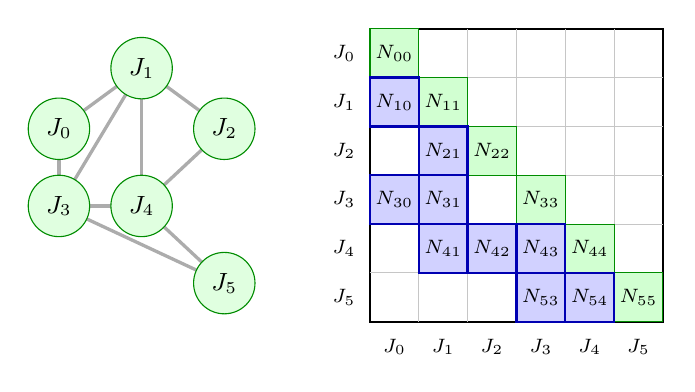
\begin{tikzpicture}[>=latex, every node/.style={font=\small}]
  % Left: joint graph.  Right: the same graph as block sparsity.
  % Edge list in both panels: 01, 12, 03, 13, 14, 24, 34, 35, 45.
  \begin{scope}[shift={(0,0.9)},x=0.70cm,y=0.70cm]
    \draw[very thick,gray!65] (0,1.4)--(1.5,2.5); % 01
    \draw[very thick,gray!65] (1.5,2.5)--(3.0,1.4); % 12
    \draw[very thick,gray!65] (0,1.4)--(0,0.0); % 03
    \draw[very thick,gray!65] (1.5,2.5)--(0,0.0); % 13
    \draw[very thick,gray!65] (1.5,2.5)--(1.5,0.0); % 14
    \draw[very thick,gray!65] (3.0,1.4)--(1.5,0.0); % 24
    \draw[very thick,gray!65] (0,0.0)--(1.5,0.0); % 34
    \draw[very thick,gray!65] (0,0.0)--(3.0,-1.4); % 35
    \draw[very thick,gray!65] (1.5,0.0)--(3.0,-1.4); % 45
    \foreach \name/\x/\y in {J_0/0/1.4,J_1/1.5/2.5,J_2/3.0/1.4,
                               J_3/0/0.0,J_4/1.5/0.0,J_5/3.0/-1.4}
      \node[circle,draw=green!55!black,fill=green!12,minimum size=0.78cm,
            inner sep=0pt] at (\x,\y) {$\name$};
  \end{scope}
  \begin{scope}[shift={(3.95,3.15)},x=0.62cm,y=0.62cm]
    % Matrix coordinates: row r is drawn at vertical coordinate -r.
    % The upper triangle is white because N is symmetric and only the lower
    % triangle is stored/displayed; no artificial triangular fill is used.
    \draw[thick] (0,0) rectangle (6,-6);
    \foreach \x in {1,...,5} \draw[gray!45] (\x,0)--(\x,-6);
    \foreach \r in {1,...,5} \draw[gray!45] (0,-\r)--(6,-\r);
    \foreach \r in {0,...,5} {
      \foreach \c in {0,...,5} {
        \pgfmathtruncatemacro{\y}{-\r}
        \ifnum\c=\r
          \path[fill=green!18,draw=green!55!black] (\c,\y) rectangle ++(1,-1);
          \node[font=\scriptsize] at (\c+0.5,\y-0.5) {$N_{\r\r}$};
        \fi
      }
    }
    % One blue lower-triangle block per graph edge.
    \foreach \r/\c in {1/0,2/1,3/0,3/1,4/1,4/2,4/3,5/3,5/4} {
      \pgfmathtruncatemacro{\y}{-\r}
      \path[fill=blue!18,draw=blue!70!black,thick] (\c,\y) rectangle ++(1,-1);
      \node[font=\scriptsize] at (\c+0.5,\y-0.5) {$N_{\r\c}$};
    }
    \foreach \i in {0,...,5} {
      \node[font=\scriptsize,anchor=east] at (-0.10,-\i-0.5) {$J_{\i}$};
      \node[font=\scriptsize,anchor=north] at (\i+0.5,-6.15) {$J_{\i}$};
    }
  \end{scope}
\end{tikzpicture}}
\caption{Left panel: joint-sharing graph. Right panel: corresponding conceptual block matrix
representation. Each graph edge $J_i$--$J_j$ produces the symmetric matrix
blocks $N_{ij}$ and $N_{ji}$; only the lower-triangle block $N_{\max(i,j),\min(i,j)}$
is shown in blue. Green cells are diagonal blocks, and the white upper triangle
is omitted because $N$ is symmetric. Symbolic elimination permutes these joint
blocks and stores only the present matrix blocks and filled factor blocks.}
\label{fig:factorization}
\end{figure}

% =============================================================================
\section{GPU Implementation}
\label{sec:gpu}

All per-step solver state remains on the GPU. The unilateral path maps contacts
to parallel work and applies the Delassus operator matrix-free: impulses scatter
to body-velocity increments, which the incident constraints then gather.
Cone projections and block-diagonal preconditioners use contact-local data.
Warm starts reuse impulses through contact correspondence, while step lengths,
residuals, and convergence decisions stay on the device.

For the bilateral path, ordering and symbolic fill are prepared once per
topology. Numerical assembly, $LDL^\top$ factorization, and the forward,
diagonal, and backward solves execute on the GPU. Homogeneous batched worlds
share symbolic indices while retaining separate numerical values. Matrix and
factor storage follow the filled block pattern described in \Cref{sec:direct}.

Force assembly, constraint solves, and integration are captured in CUDA graphs
with preallocated buffers. A fixed iteration cap preserves a static graph, and
a device flag masks later iterations after convergence. Where conditional graph
nodes are available, bounded solver and line-search loops can terminate on the
device. Shared-body and scalar reductions use scaled 64-bit integer atomics so
their result is independent of GPU accumulation order; the scale keeps
quantization below the solver tolerance without overflowing
(\Cref{app:determinism}). This deterministic guarantee covers solver reductions
for a fixed input and execution configuration, not the complete collision,
integration, or learning process.

% =============================================================================
\FloatBarrier
\section{Results}
\label{sec:results}

The evaluation progresses from controlled numerical validation to complete
robot-learning workloads. Pendulum trajectories test the bilateral
maximal-coordinate solve against high-accuracy reference data. Frozen box
stacks isolate the residual--cost behavior of the three contact solvers;
fixed-base tests measure batched frame time; and policy experiments exercise
tree-structured and closed-loop robots. The fixed-base measurements use an
NVIDIA L40, and the fixed-contact timings are medians of repeated synchronized
solves. Comparisons with MJWarp retain each implementation's coordinate,
contact, collision, and integration path, so the reported timings cover
complete simulation pipelines rather than identical numerical kernels.

\subsection{Analytical validations}
\label{sec:analytical-validations}

\subsubsection{Single-pendulum ODE validation}
\label{sec:pendulum-results}

We first validate the bilateral direct solve on a physical compound pendulum
with a fixed support and one revolute joint. The link uses the same capsule
geometry and mass properties as the existing Newton pendulum example. We disable
joint damping, external torque, and contacts, release the link from
$45^\circ$, and simulate for $4\,\mathrm{s}$ at $240\,\mathrm{Hz}$ with four
substeps. As a reference, we numerically integrate the exact reduced equation
of motion
\[
 I_p\ddot\theta + m g d\sin\theta=0,
 \qquad I_p=I_{\mathrm{COM}}+m d^2,
\]
where $d$ is the pivot-to-center-of-mass distance. The reference is a numerical
ODE solution, not a closed-form trajectory: classical fourth-order Runge--Kutta
integration is evaluated at the recorded output times. The reference and both
simulators use the same initial angle and zero angular velocity. We record the
joint angle, reconstructed anchor-point separation, and mechanical energy
$E=T+V$.

\begin{figure}[t]
  \centering
  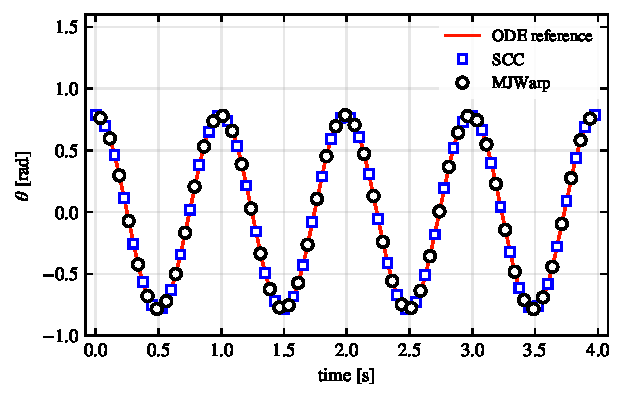
\includegraphics[width=0.32\linewidth]{results/pendulum_validation/figures/pendulum_analytical_angle.pdf}\hfill
  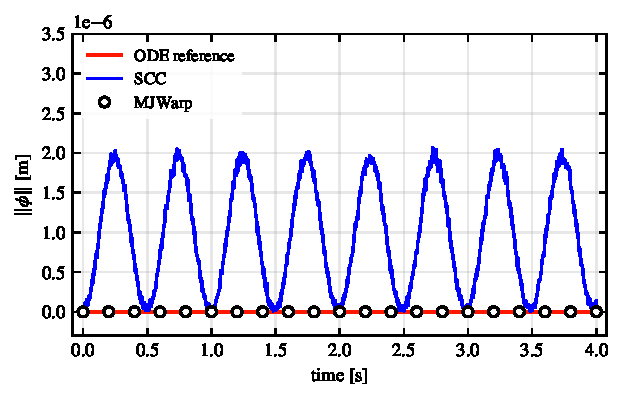
\includegraphics[width=0.32\linewidth]{results/pendulum_validation/figures/pendulum_analytical_joint_violation.pdf}\hfill
  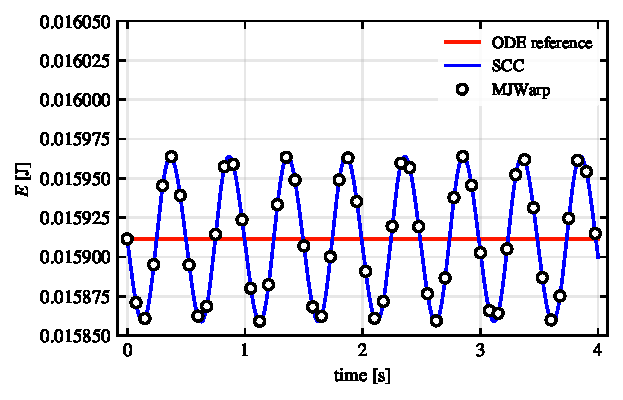
\includegraphics[width=0.32\linewidth]{results/pendulum_validation/figures/pendulum_analytical_total_energy.pdf}
  \caption{ODE-reference validation of the compound pendulum over the first
  $4\,\mathrm{s}$. From left to right: joint angle, joint-anchor separation,
  and total mechanical energy. SCC uses the sparse direct joint solve with
  $\alpha=0$, regularization $10^{-6}$, one coupling sweep, and semi-implicit
  integration. MJWarp uses its Newton solve with Euler integration, one outer
  iteration, and four line-search iterations. Both simulations disable
  contacts, damping, armature, and external torque and use $240\,\mathrm{Hz}$
  with four substeps; the reference uses fixed-step RK4.}
  \label{fig:pendulum-analytical}
\end{figure}

Both trajectories follow the reference over the four-second horizon. The SCC
anchor-point separation remains on the micrometre scale, and its angle error is
below one degree in the plotted interval. The displayed energy curves are nearly
coincident. MJWarp eliminates this tree joint in reduced coordinates, so a zero
anchor-separation residual is a representational property rather than evidence
that its time integration is exact.

\subsubsection{Double-pendulum ODE validation}
\label{sec:double-pendulum-results}

The two-link pendulum tests coupled bilateral dynamics. The system is simulated
for $4\,\mathrm{s}$ at
$240\,\mathrm{Hz}$ using four substeps per frame, with zero joint damping,
zero armature, zero external torque, and no contacts. SCC uses the sparse direct
joint solve with $\alpha=0$, regularization $10^{-6}$, one coupling sweep,
and semi-implicit integration. MJWarp uses its Newton solve with RK4 integration,
one nonlinear iteration, and four line-search iterations. The reference is the
coupled Euler--Lagrange ODE integrated with the adaptive DOP853 method at relative
and absolute tolerances $2\times10^{-11}$ and $2\times10^{-13}$, respectively.

\begin{figure}[t]
  \centering
  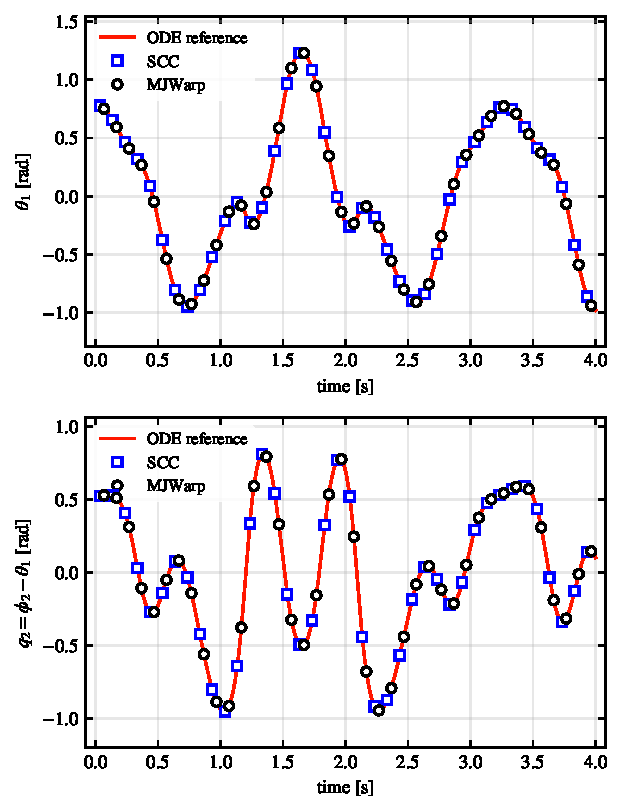
\includegraphics[width=0.32\linewidth]{results/double_pendulum_validation/figures/double_pendulum_angles.pdf}\hfill
  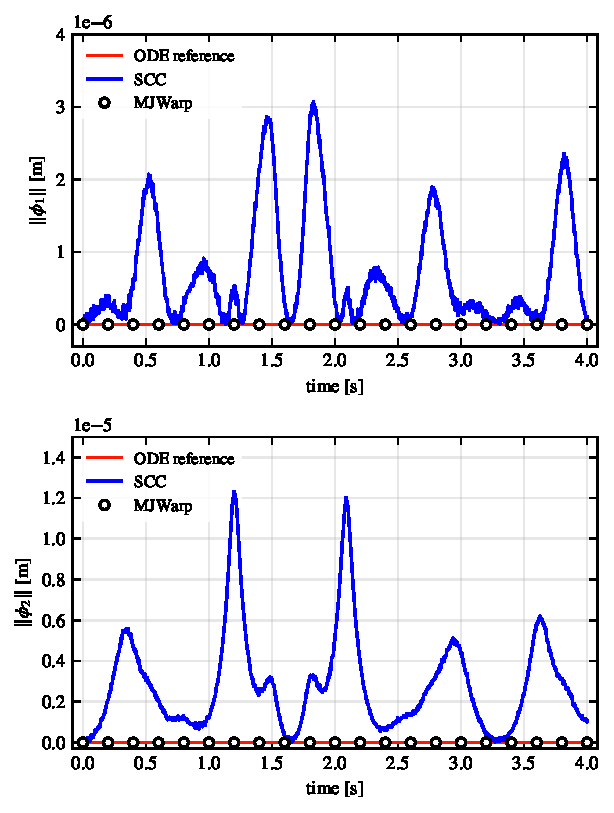
\includegraphics[width=0.32\linewidth]{results/double_pendulum_validation/figures/double_pendulum_violations.pdf}\hfill
  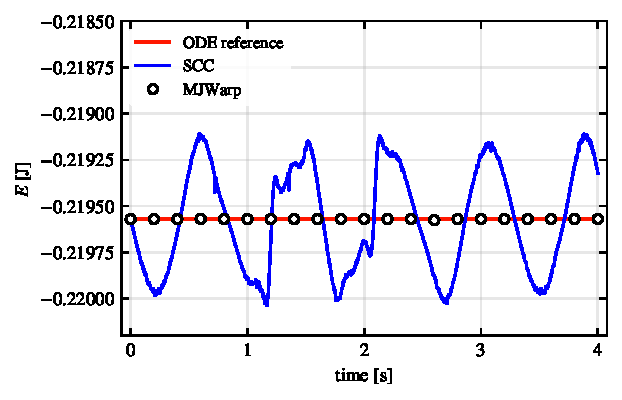
\includegraphics[width=0.32\linewidth]{results/double_pendulum_validation/figures/double_pendulum_energy.pdf}
  \caption{ODE-reference validation of the double pendulum over the first
  $4\,\mathrm{s}$. From left to right: the two generalized joint angles, the
  two reconstructed joint-position violations, and total mechanical energy.
  SCC uses a sparse direct bilateral solve with $\alpha=0$, regularization $10^{-6}$, one
  coupling sweep, and semi-implicit integration. The
  MJWarp run uses the Newton solver, RK4 integration, one solver iteration,
  four line-search iterations, and disabled contacts. Both simulations use
  zero damping, zero armature, zero external torque, $240\,\mathrm{Hz}$, and
  four substeps; the ODE-reference curve uses DOP853 with relative and absolute
  tolerances $2\times10^{-11}$ and $2\times10^{-13}$, respectively.}
  \label{fig:double-pendulum-analytical}
\end{figure}

The reference integrates the coupled Euler--Lagrange equations in absolute
link angles $(\theta_1,\phi_2)$. In explicit matrix form,
\begin{equation}
\begin{bmatrix}A&C\cos(\theta_1-\phi_2)\\
C\cos(\theta_1-\phi_2)&B\end{bmatrix}
\begin{bmatrix}\ddot\theta_1\\\ddot\phi_2\end{bmatrix}
=-\begin{bmatrix}
C\sin(\theta_1-\phi_2)\dot\phi_2^2+K_1\sin\theta_1\\
-C\sin(\theta_1-\phi_2)\dot\theta_1^2+K_2\sin\phi_2
\end{bmatrix},
\end{equation}
where $A=I_1+m_2l_1^2$, $B=I_2$, $C=m_2l_1r_2$,
$K_1=g(m_1r_1+m_2l_1)$, and $K_2=gm_2r_2$. The model's second generalized
coordinate is relative, so the reported coordinates are
$q_1=\theta_1$ and $q_2=\phi_2-\theta_1$. This matches both the initial
configuration and the coordinate convention used by both simulators. The
trajectories reproduce the coupled motion, but MJWarp's RK4 reduced-coordinate
configuration remains closer to the ODE reference over this horizon. SCC
maintains reconstructed joint violations on the order of $10^{-5}\,\mathrm{m}$.
As in the single-link case, zero MJWarp joint violation follows from coordinate
elimination and is not directly comparable with a maximal-coordinate residual.

\subsubsection{Contact-solver comparison on box stacks}
\label{sec:box-results}

We compare the three matrix-free cone solvers on a controlled resting-contact
problem containing either five or ten identical boxes above a
horizontal ground plane. Each box has side length $s=0.2\,\mathrm{m}$, mass
$1\,\mathrm{kg}$, and diagonal inertia $\frac{1}{6}ms^2$; the friction
coefficient is $\mu=0.75$. The contact model uses a $1\,\mathrm{mm}$ gap and
margin, and the stack is simulated at $\Delta t=1/60\,\mathrm{s}$ under gravity
$g=9.81\,\mathrm{m\,s^{-2}}$. The five- and ten-box scenes contain 20 and 40
active contact points, respectively.

To compare methods on exactly the same problem, an APGD-driven trajectory is
advanced for 90 frames and the complete state at frame 90 is frozen. Collision
geometry and the resulting contact set are therefore identical for all methods.
Each solver starts from that state with a zero contact warm start and is run with
increasing iteration caps. The plotted float32 residual is the normal
complementarity diagnostic
\begin{equation}
r_{\mathrm{FB},n}=\max_i
\left|\lambda_{n,i}+u_{n,i}-\sqrt{\lambda_{n,i}^2+u_{n,i}^2}\right|,
\qquad \mathbf u=\Aop\blam+\rhs .
\label{eq:res_comp}
\end{equation}
This diagnostic does not by itself measure full tangential cone stationarity;
the natural residual in \eqref{eq:res_pg} includes both normal and tangential
stationarity. Timing encloses the complete contact solve
with CUDA synchronization and reports the median of 15 repeats at each cap.
Exact float32 zeros are omitted from the logarithmic plot rather than replaced
by an arbitrary floor.

The bilateral block uses a sparse direct solve with $\alpha=0.01$, recovery speed $0.05$,
and regularization $10^{-6}$. Contact solves use $\omega=0.5$, relaxation
$0.9$, $\alpha=0.001$, recovery speed $0.5$, regularization $10^{-4}$,
compliance $10^{-9}$, disabled warm starting, and disabled early exit. These
settings are fixed between scenes. Contact iteration caps are logarithmically
spaced from 1 to 150.

\begin{figure}[t]
  \centering
  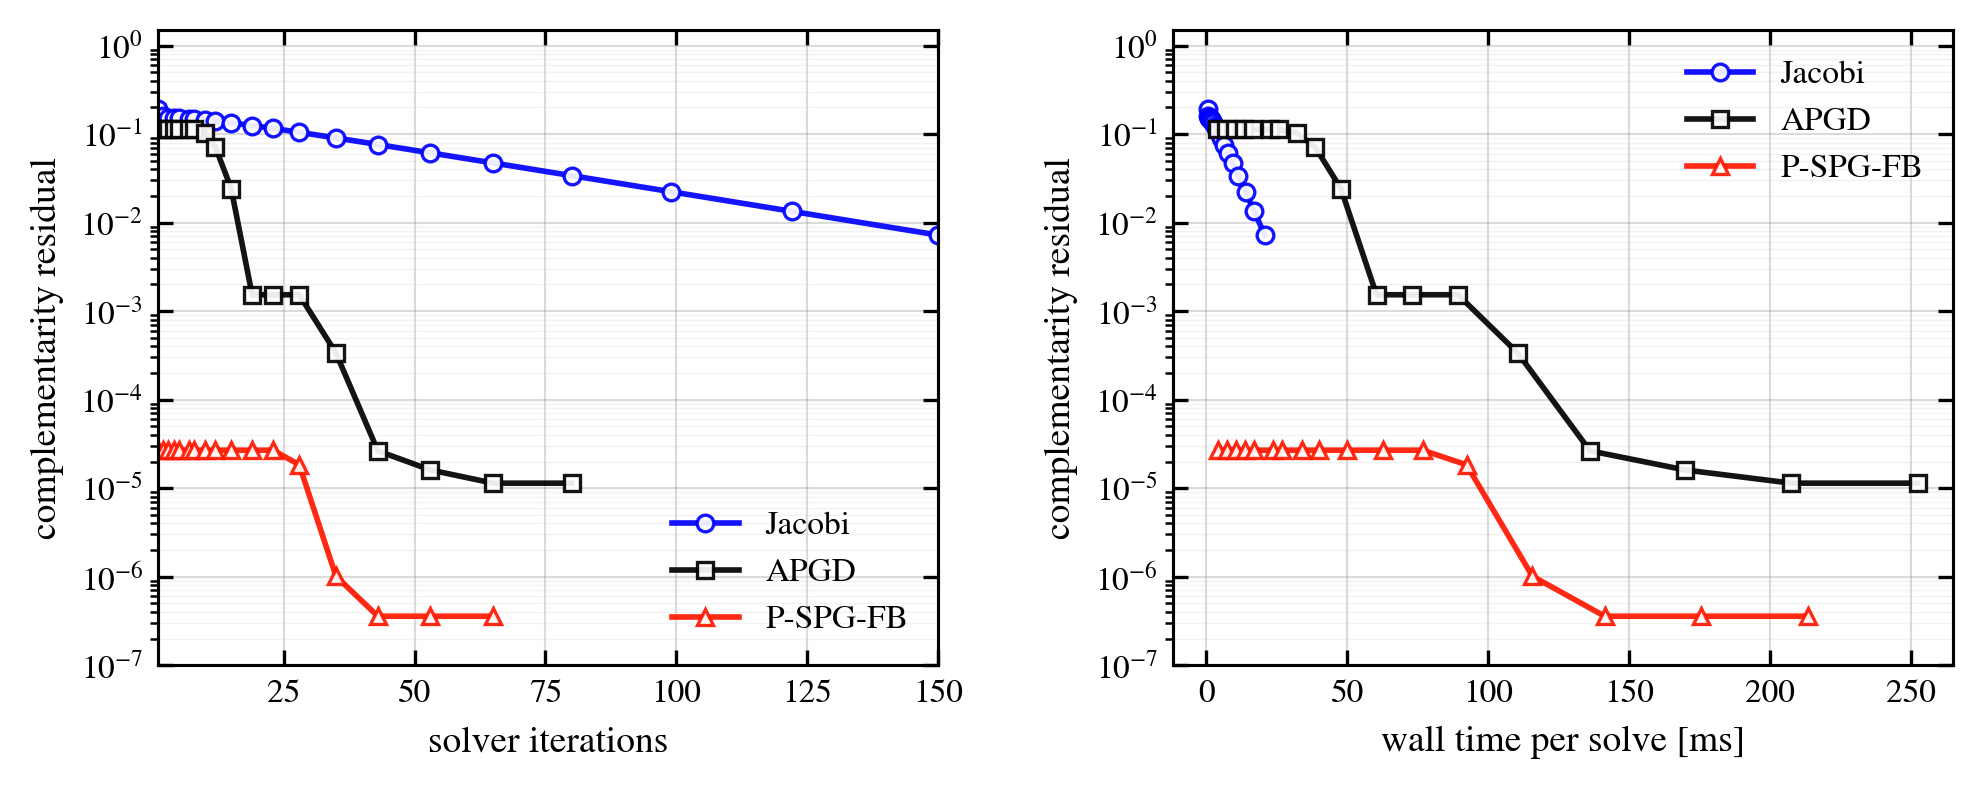
\includegraphics[width=0.99\linewidth]{results/box_stacking/figures/box_stack_5boxes_convergence.png}
  \caption{Contact-solver convergence for the five-box stack at one fixed,
  settled contact state. Left: complementarity residual versus iteration cap.
  Right: the same residual versus measured solve time. Jacobi, APGD, and
  P-SPG-FB are blue, black, and red, respectively.}
  \label{fig:box-convergence-5}
\end{figure}

\begin{figure}[t]
  \centering
  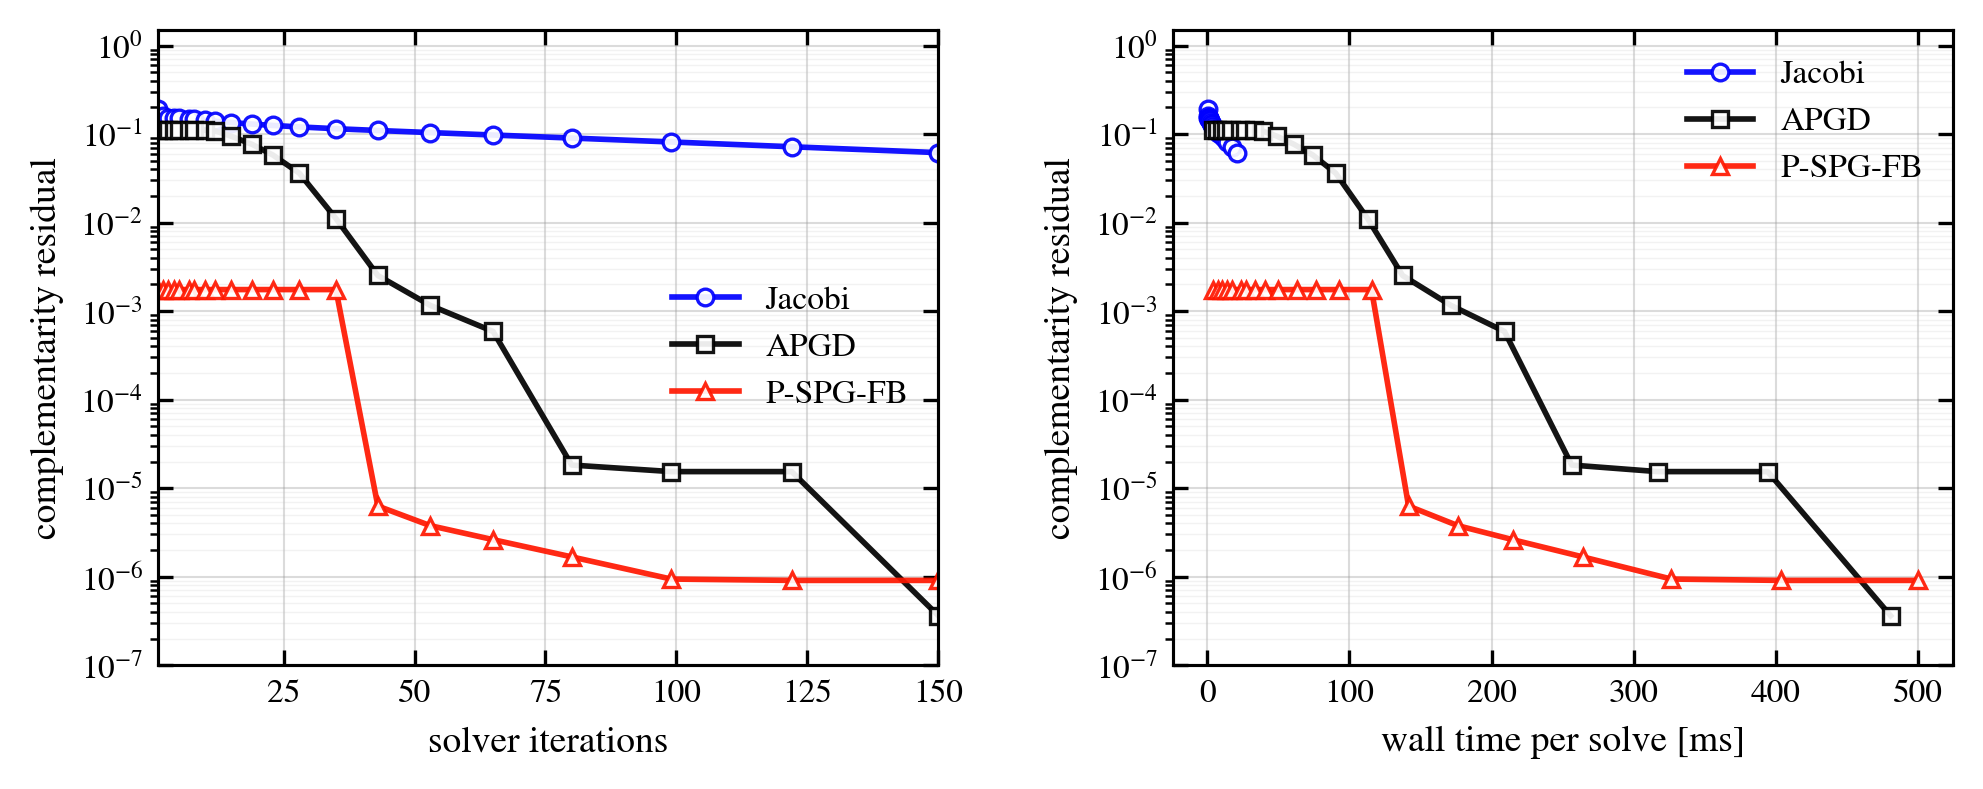
\includegraphics[width=0.99\linewidth]{results/box_stacking/figures/box_stack_10boxes_convergence.png}
  \caption{Contact-solver convergence for the ten-box stack. The protocol and
  plotting conventions are identical to \Cref{fig:box-convergence-5}; the scene
  has twice as many active contacts.}
  \label{fig:box-convergence-10}
\end{figure}

For five boxes, APGD and P-SPG-FB reduce the normal residual in fewer outer
iterations than projected Jacobi. Jacobi is much cheaper per iteration, so the
wall-time panel changes the practical comparison: line searches and momentum
improve progress per iteration but add work. The ten-box stack strengthens this
pattern; Jacobi's progress slows as impulses must propagate through more coupled
contacts. P-SPG-FB also has a much smaller residual after its first reported
outer iteration, which includes more internal work than one Jacobi update and
is therefore interpreted together with the time plot. The frozen state isolates
the convergence of one resting-contact CCP from collision detection and time
integration.

The main separation is already visible well before the 150-iteration plotting
limit. At the 80-iteration sample for ten boxes, the normal residual is
$9.02\times10^{-2}$ for Jacobi, $1.83\times10^{-5}$ for APGD, and
$1.67\times10^{-6}$ for P-SPG-FB. APGD and P-SPG-FB are therefore approximately
3.7 and 4.7 orders of magnitude below Jacobi at this point. The corresponding
recorded solve times are $11.5\,\mathrm{ms}$, $256.4\,\mathrm{ms}$, and
$264.1\,\mathrm{ms}$. At this matched iteration cap, APGD and P-SPG-FB
therefore take 22.2 and 22.9 times as long as Jacobi, respectively, while
achieving substantially greater residual reduction.

For this scene the analytical equilibrium centers are
\[
  \mathbf p_i^\star=(0,0,0.101+0.202i)^\mathsf T,\qquad
  \mathbf v_i^\star=\mathbf 0,\qquad i=0,\ldots,n-1,
\]
where the $0.202\,\mathrm{m}$ center spacing comprises the $0.2\,\mathrm{m}$
side length and two $1\,\mathrm{mm}$ contact margins. We report
$\Delta p_i=\|\mathbf p_i-\mathbf p_i^\star\|_2$ and a stored six-component
velocity-state norm for each box after 150 contact iterations. The position
error is a physical error relative to the stated equilibrium. The velocity norm
concatenates translational and angular components with different units and is
therefore a within-scene numerical diagnostic, not a dimensionally homogeneous
physical norm.

\begin{figure}[t]
  \centering
  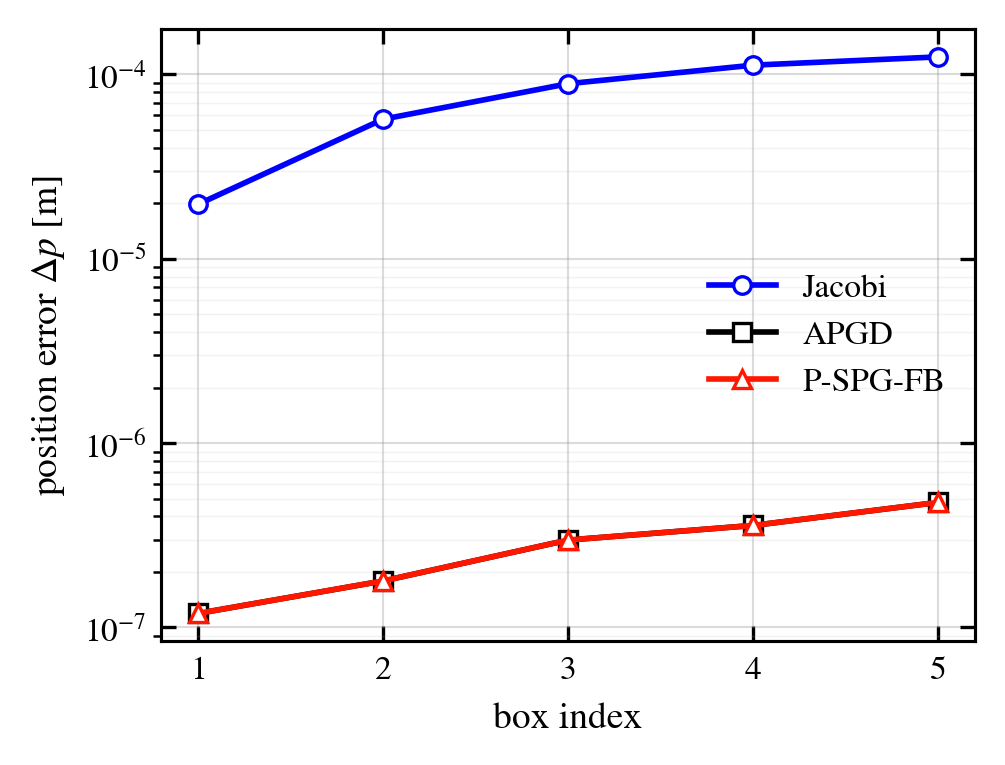
\includegraphics[width=0.48\linewidth]{results/box_stacking/figures/box_stack_5boxes_position_error.png}\hfill
  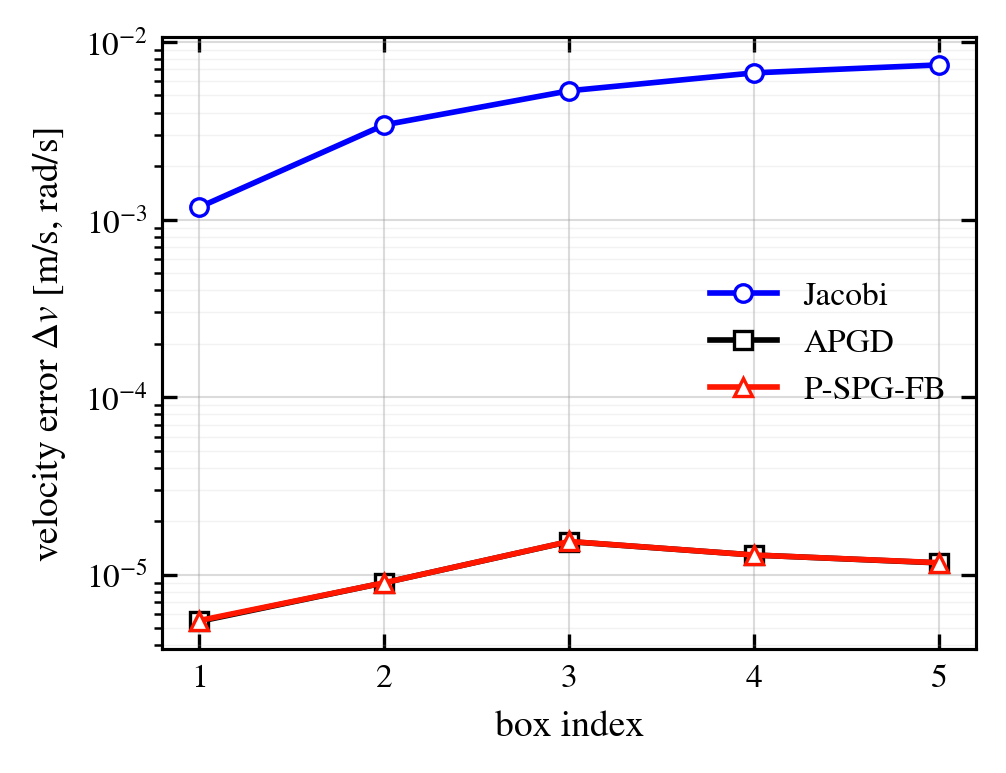
\includegraphics[width=0.48\linewidth]{results/box_stacking/figures/box_stack_5boxes_velocity_error.png}
  \caption{Five-box equilibrium diagnostics after 150 contact iterations:
  position error relative to the stated centers (left) and the stored mixed-unit
  velocity-state norm (right), versus box index.}
  \label{fig:box-errors-5}
\end{figure}

\begin{figure}[t]
  \centering
  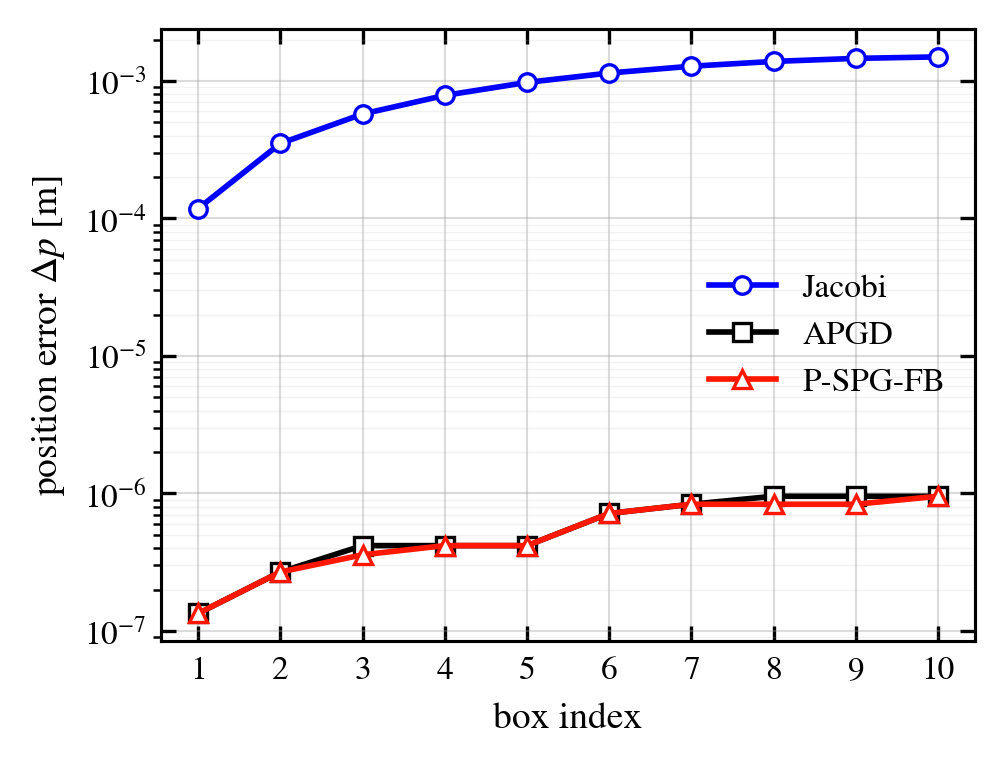
\includegraphics[width=0.48\linewidth]{results/box_stacking/figures/box_stack_10boxes_position_error.png}\hfill
  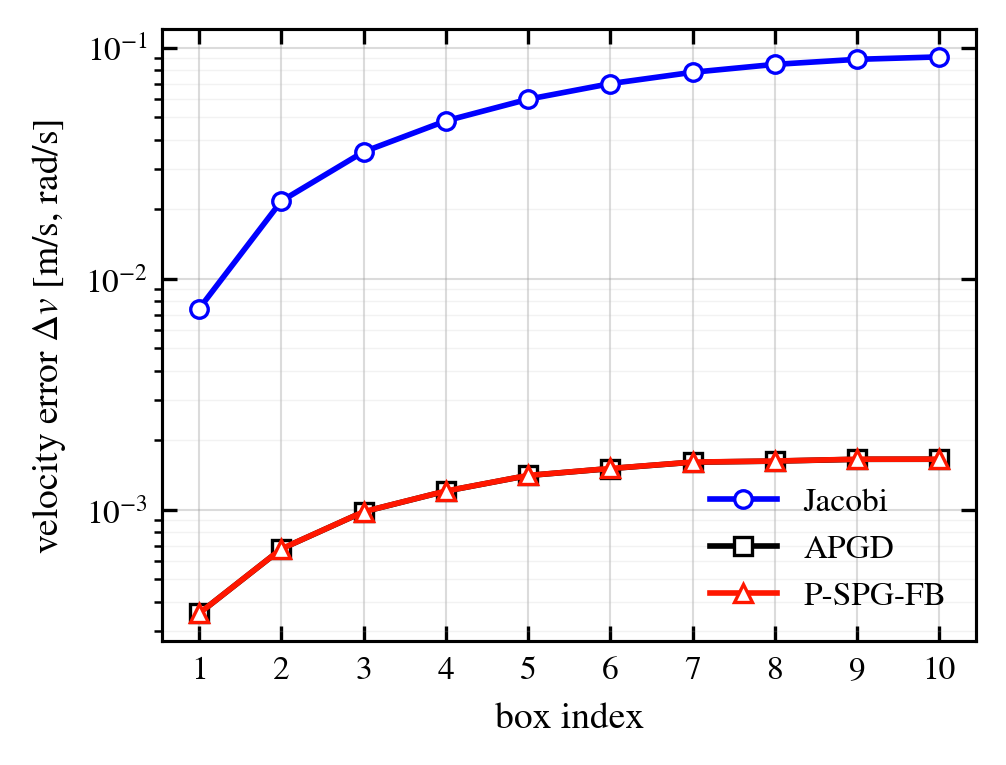
\includegraphics[width=0.48\linewidth]{results/box_stacking/figures/box_stack_10boxes_velocity_error.png}
  \caption{Ten-box equilibrium diagnostics after 150 contact iterations.
  The same definitions and solver colors as in
  \Cref{fig:box-errors-5} are used.}
  \label{fig:box-errors-10}
\end{figure}

APGD and P-SPG-FB nearly overlap in the equilibrium plots at the selected
iteration budget, so their visible distinction is convergence cost rather than
the final resting configuration. Jacobi retains a larger velocity-state norm,
especially in the ten-box stack, consistent with its slower residual decrease.

\subsubsection{Actuation-path verification}
\label{sec:actuation-verification}

We verify target propagation through the maximal-coordinate actuation path on
fixed-base G1 and MuJoCo Humanoid models. Every finite-limited scalar
generalized coordinate is commanded simultaneously from its imported model
pose to its own mid-range target. For a coordinate with finite bounds,
$q_{\mathrm{mid}}=(q_{\min}+q_{\max})/2$ and
$\hat q=2(q-q_{\min})/(q_{\max}-q_{\min})-1$, so the target is
$\hat q=0$. The G1 1-s and Humanoid 0.5-s trajectories in \Cref{fig:actuation-verification}
show a readable right-side/waist subset; the accompanying records include all
commanded finite-limited coordinates. Both trajectories remain finite, satisfy
the normalized limits, and approach their midpoint targets. The Humanoid
abdomen, ankle, and shoulder joints are represented as two-axis joints and
are reported in their serial generalized-coordinate chart.

\begin{figure}[t]
  \centering
  \begin{minipage}[b]{0.49\linewidth}
    \centering
    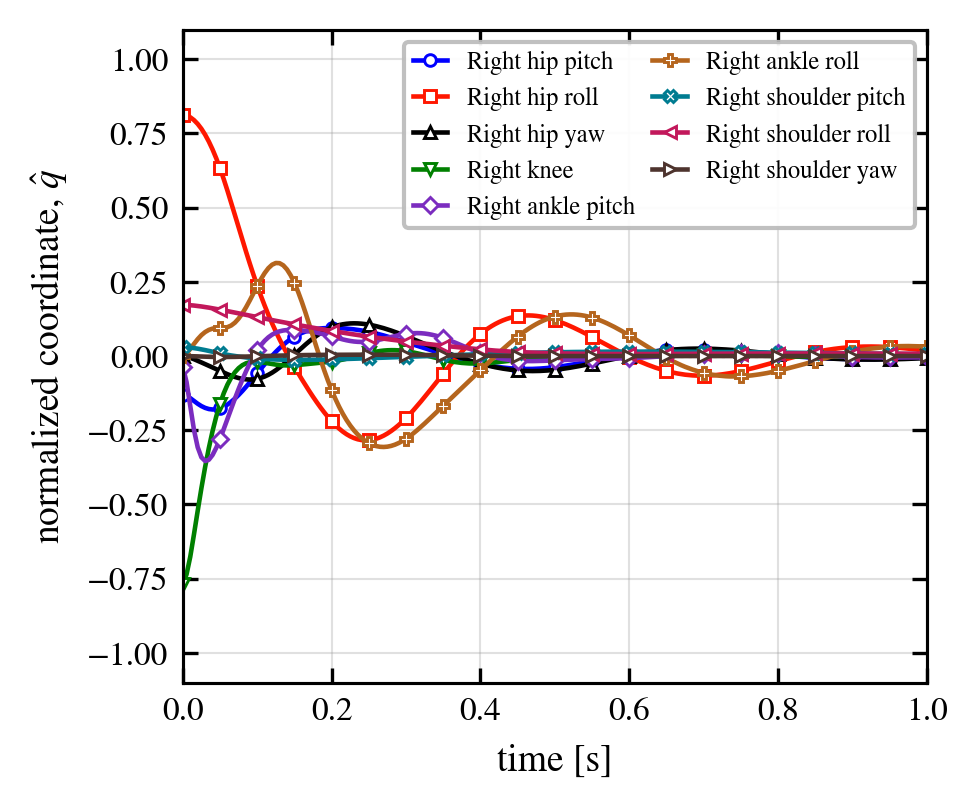
\includegraphics[width=\linewidth]{results/joint_solver_scaling/figures/g1_midrange_dvi_1s_verification.png}
  \end{minipage}\hfill
  \begin{minipage}[b]{0.49\linewidth}
    \centering
    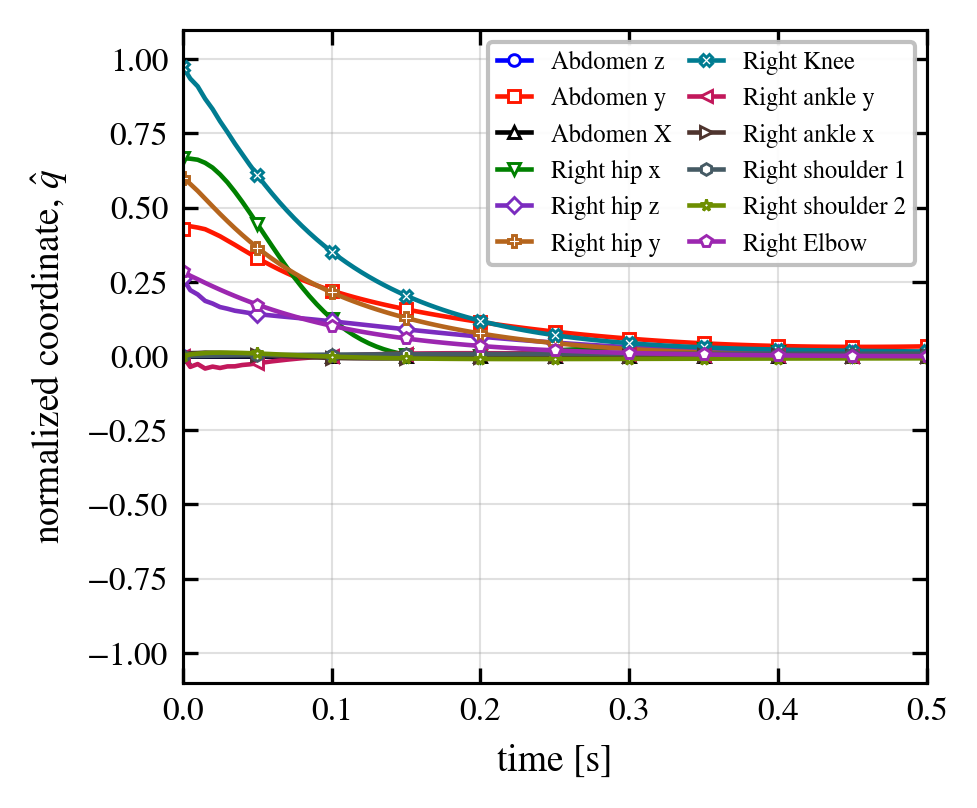
\includegraphics[width=\linewidth]{results/joint_solver_scaling/figures/humanoid_midrange_dvi_0p5s_verification.png}
  \end{minipage}
  \caption{SCC fixed-base mid-range actuation verification.
  \textbf{Left:} G1 over $1\,\mathrm{s}$. \textbf{Right:} MuJoCo Humanoid over $0.5\,\mathrm{s}$. Every finite-limited
  generalized coordinate is commanded to its individual limit midpoint from
  the imported model pose; displayed curves are a readable right-side/waist
  subset, and $\hat q=0$ (dotted line) is the target. This is a target-
  propagation diagnostic, not a solver-performance or contact-accuracy
  comparison.}
  \label{fig:actuation-verification}
\end{figure}
\FloatBarrier

\subsection{Scaling Analysis}
\label{sec:joint-solver-scaling}

We next measure fixed-base CUDA-graph frame time on an NVIDIA L40 for
G1 and MuJoCo Humanoid using the same midpoint targets. Two alternating graphs
advance the state buffers; each captured SCC frame includes force clearing,
Newton collision-pipeline processing, and one SCC substep, whereas MJWarp uses
its standard collision and dynamics path. The scenario and timing boundary are
matched, while the internal numerical work remains specific to each method.
Inverse kinematics,
policy inference, observations, rewards, resets, and manager overhead are
excluded. Each 1-s campaign uses 200 physics frames at 200 Hz, 20 ordinary
warmup frames, 20 graph-warm replay pairs, and 180 timed graph replays with one
trailing synchronization.

\begin{figure}[t]
  \centering
  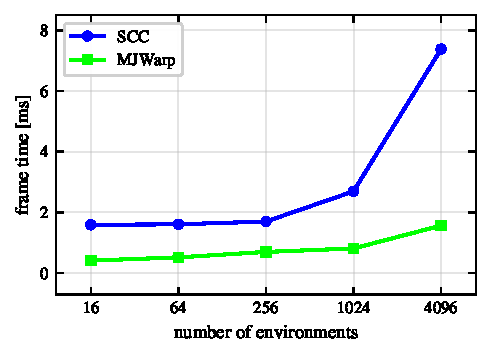
\includegraphics[width=0.49\linewidth]{results/joint_solver_scaling/figures/g1_dvi_mjwarp_cudagraph_scaling.pdf}\hfill
  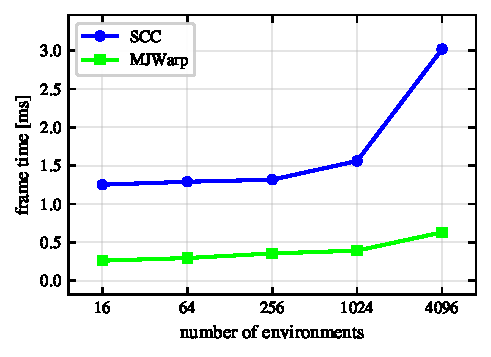
\includegraphics[width=0.49\linewidth]{results/joint_solver_scaling/figures/humanoid_dvi_mjwarp_cudagraph_scaling.pdf}
  \caption{Fixed-base CUDA-graph scaling on an NVIDIA L40 with midpoint targets:
  \textbf{left} G1 and \textbf{right} MuJoCo Humanoid. Each curve reports the
  GPU frame time of the complete captured path: SCC uses maximal-coordinate dynamics
  with the Newton collision pipeline, while MJWarp uses reduced-coordinate
  MuJoCo Warp dynamics and collision. The figure is a fixed-base solver
  microbenchmark, not end-to-end RL throughput.}
  \label{fig:g1-humanoid-scaling}
\end{figure}

Both implementations show a nearly flat small-batch regime followed by greater
frame time as the batch reaches 1024 and 4096 environments. MJWarp has lower
frame time at every reported batch size for both tree-structured models, with a
larger absolute separation on G1 than on Humanoid. Because each curve includes
its implementation's collision processing and dynamics path, the comparison
characterizes the complete fixed-base simulation step rather than a single
factorization or kernel.
\FloatBarrier

\subsection{Hoberman sphere}
\label{sec:hoberman-sphere}

\subsection{Reinforcement learning benchmarks}
\label{sec:rl-results}

We evaluate end-to-end reinforcement learning (RL) workloads from Isaac Lab on
Ant, direct MuJoCo Humanoid, H1, G1, Go2, and Anymal C. Each comparison uses
seed 42, a shared PPO configuration within the environment, and the same task
specification. The curves report mean episode reward with exponential
moving-average smoothing (span 35) and a rolling within-run standard-deviation
band.

\Cref{tab:rl-solver-parameters} reports the physics substeps and the
Newton--SCC contact-iteration budget, outer coupling iterations, and bilateral
post-stabilization setting. Jacobi and MJWarp use matched substep counts in every
environment: two for direct MuJoCo Humanoid and one for the other five tasks.
MJWarp uses its standard solver configuration; its settings are consequently
not numerically equivalent to SCC iteration counts.

\begin{table*}[t]
\centering
\caption{Solver settings for the reward curves in \Cref{fig:rl-all-environments}. The
substep count is the number of physics solves per simulation step. MJWarp uses
its native solver configuration and therefore has no corresponding SCC
contact-iteration, coupling, or final bilateral-correction settings. The
APGD and P-SPG-FB rows use the same substep count as the matched Jacobi row.}
\label{tab:rl-solver-parameters}
\small
\begin{tabular}{llrrrr}
\toprule
Environment & Solver & Substeps & Contact iters. & Coupling & Final corr. \\
\midrule
Ant & Jacobi & 1 & 10 & 1 & yes \\
Ant & APGD & 1 & 10 & 1 & yes \\
Ant & P-SPG-FB & 1 & 10 & 1 & yes \\
Ant & MJWarp & 1 & -- & -- & -- \\
Humanoid direct & Jacobi & 2 & 10 & 1 & yes \\
Humanoid direct & APGD & 2 & 10 & 1 & yes \\
Humanoid direct & P-SPG-FB & 2 & 10 & 1 & yes \\
Humanoid direct & MJWarp & 2 & -- & -- & -- \\
H1 & Jacobi & 1 & 10 & 1 & no \\
H1 & APGD & 1 & 10 & 1 & no \\
H1 & P-SPG-FB & 1 & 10 & 1 & no \\
H1 & MJWarp & 1 & -- & -- & -- \\
G1 & Jacobi & 1 & 15 & 2 & no \\
G1 & APGD & 1 & 15 & 2 & no \\
G1 & P-SPG-FB & 1 & 15 & 2 & no \\
G1 & MJWarp & 1 & -- & -- & -- \\
Go2 & Jacobi & 1 & 15 & 2 & no \\
Go2 & APGD & 1 & 15 & 2 & no \\
Go2 & P-SPG-FB & 1 & 15 & 2 & no \\
Go2 & MJWarp & 1 & -- & -- & -- \\
ANYmal C & Jacobi & 1 & 20 & 2 & no \\
ANYmal C & APGD & 1 & 20 & 2 & no \\
ANYmal C & P-SPG-FB & 1 & 20 & 2 & no \\
ANYmal C & MJWarp & 1 & -- & -- & -- \\
\bottomrule
\end{tabular}
\end{table*}

% All SCC rows use sparse LDL for bilateral joints and cache_factorization=true.
% P-SPG-FB rows change only the contact solver relative to their APGD counterparts.
% Anymal C uses the manager-based flat task; its solver rows are matched.


\begin{figure*}[!htbp]
  \centering
  \begin{minipage}[t]{0.47\textwidth}
    \centering
    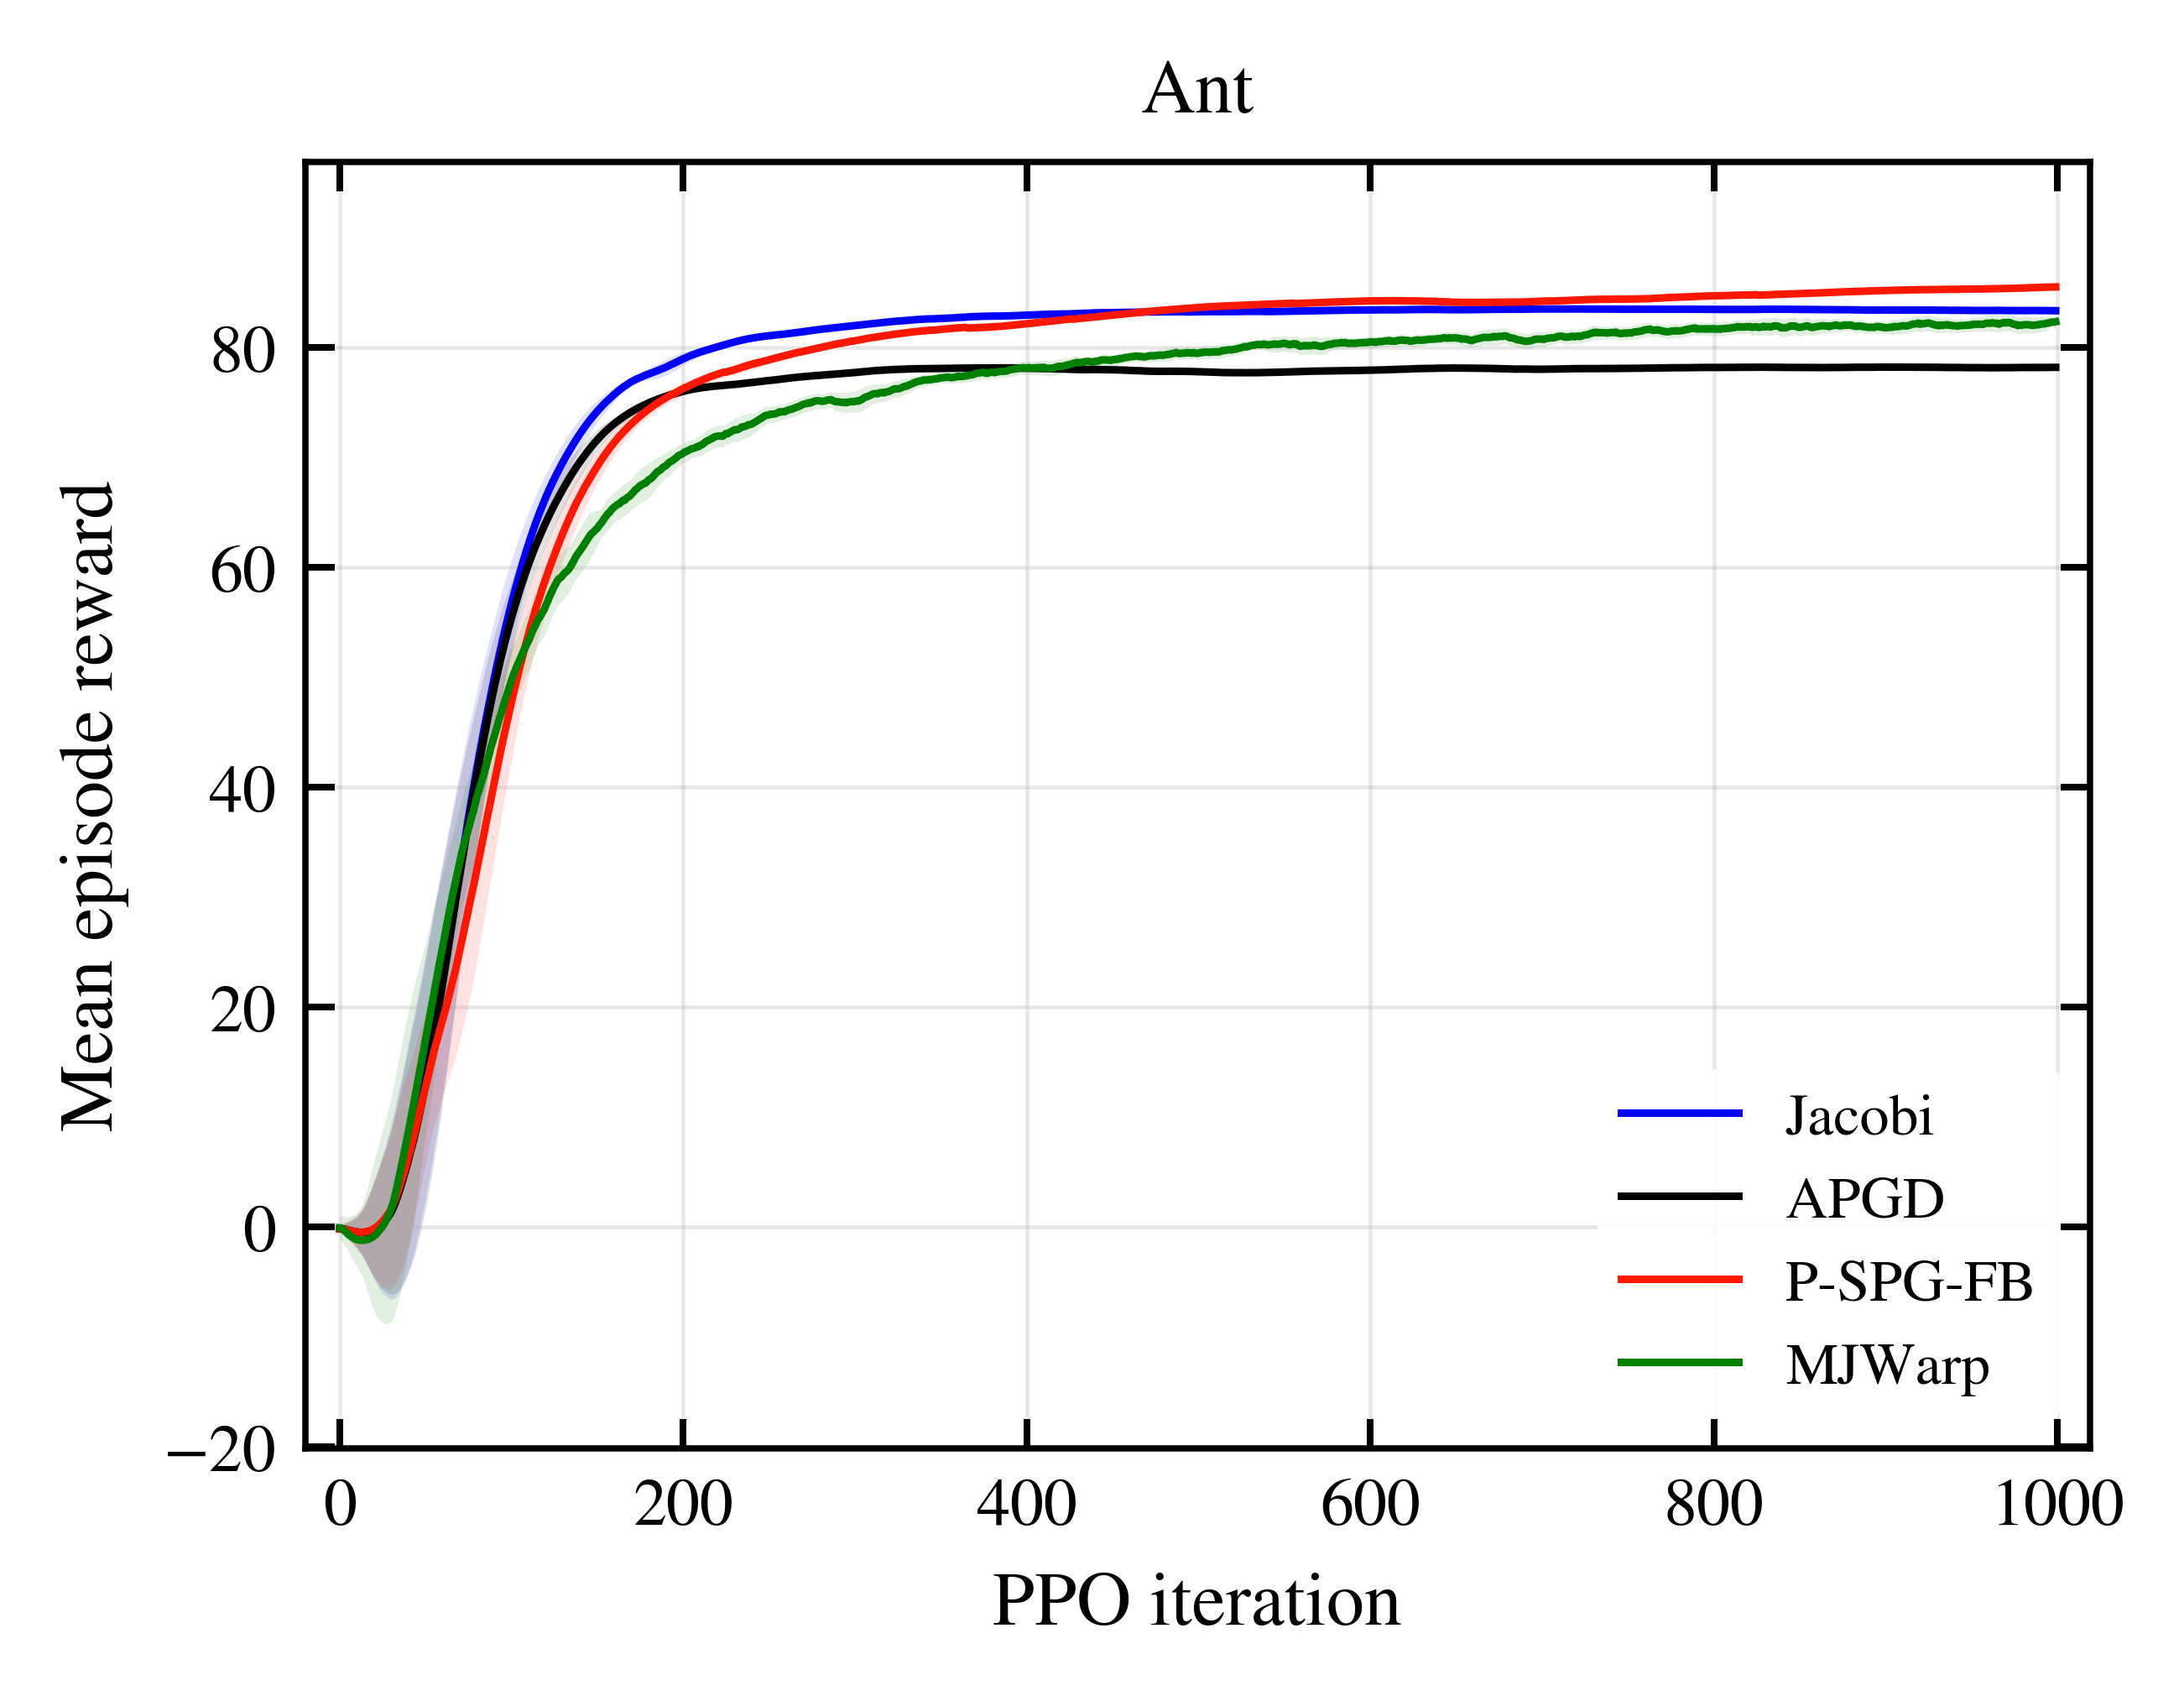
\includegraphics[width=\linewidth]{results/reinforcement_learning/figures/ant_jacobi_mjwarp_apgd_progress.png}
  \end{minipage}\hfill
  \begin{minipage}[t]{0.47\textwidth}
    \centering
    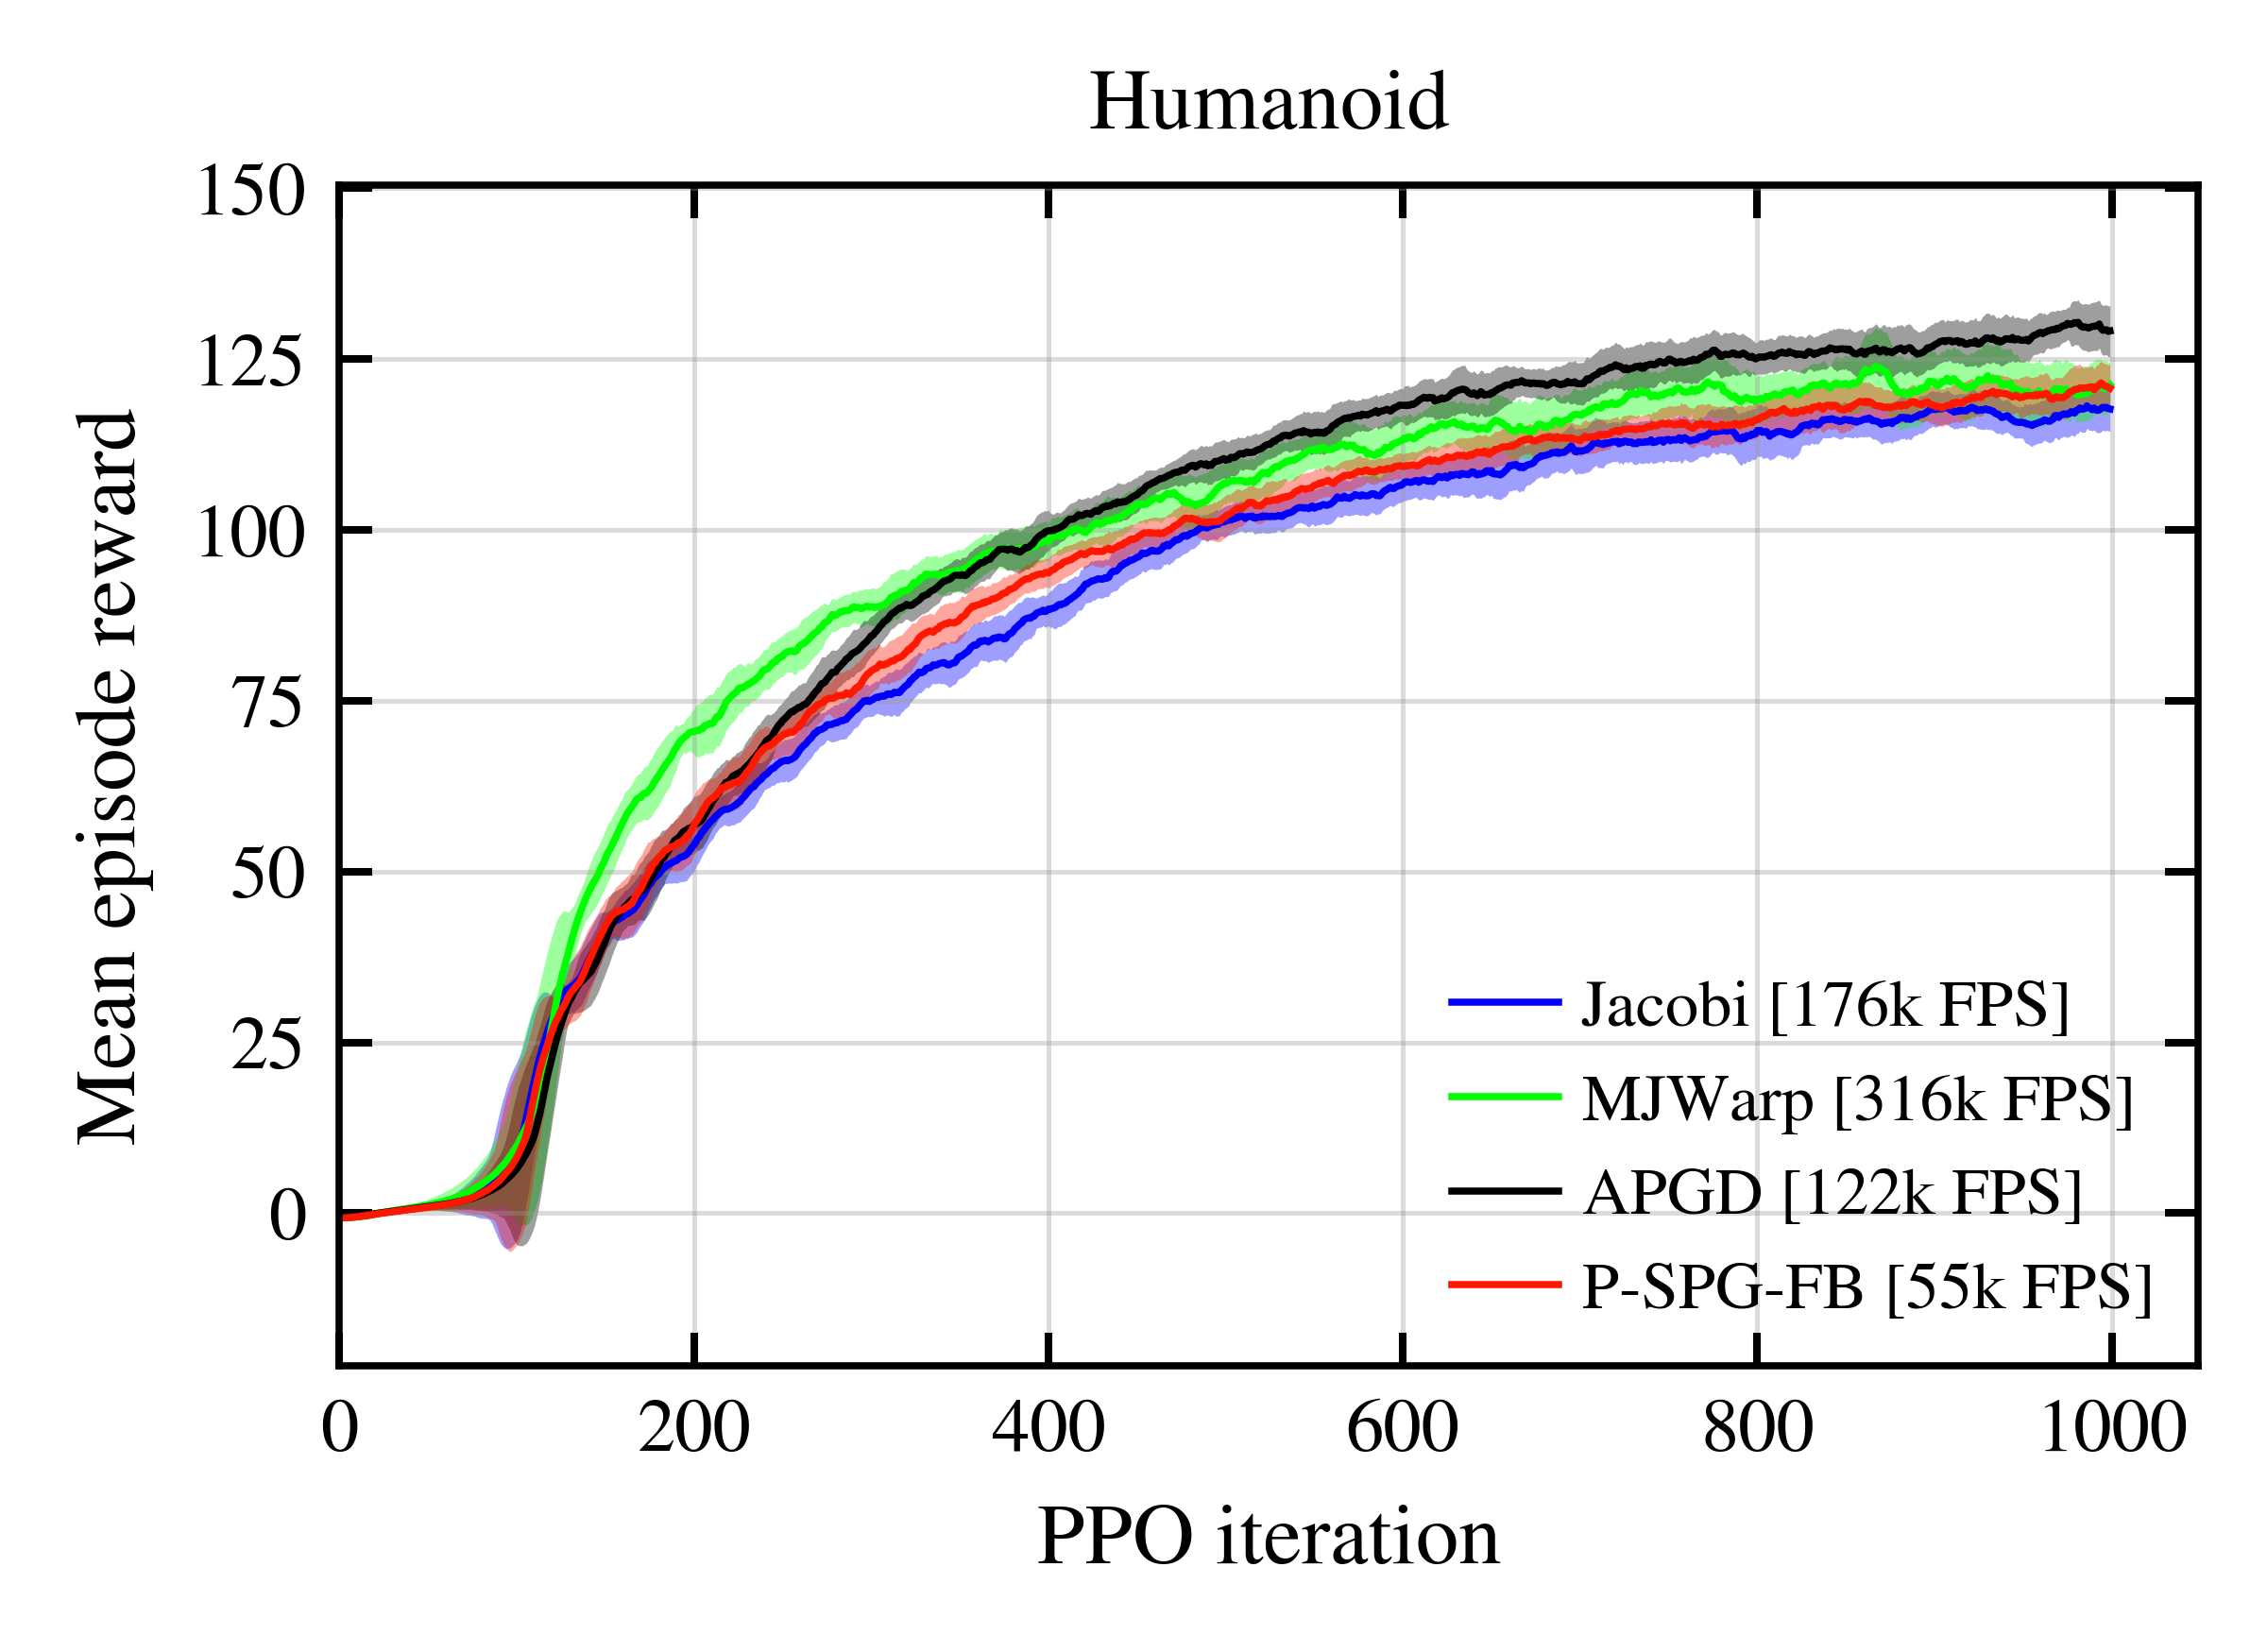
\includegraphics[width=\linewidth]{results/reinforcement_learning/figures/humanoid_jacobi_mjwarp_apgd_progress.png}
  \end{minipage}\\[4pt]
  \begin{minipage}[t]{0.47\textwidth}
    \centering
    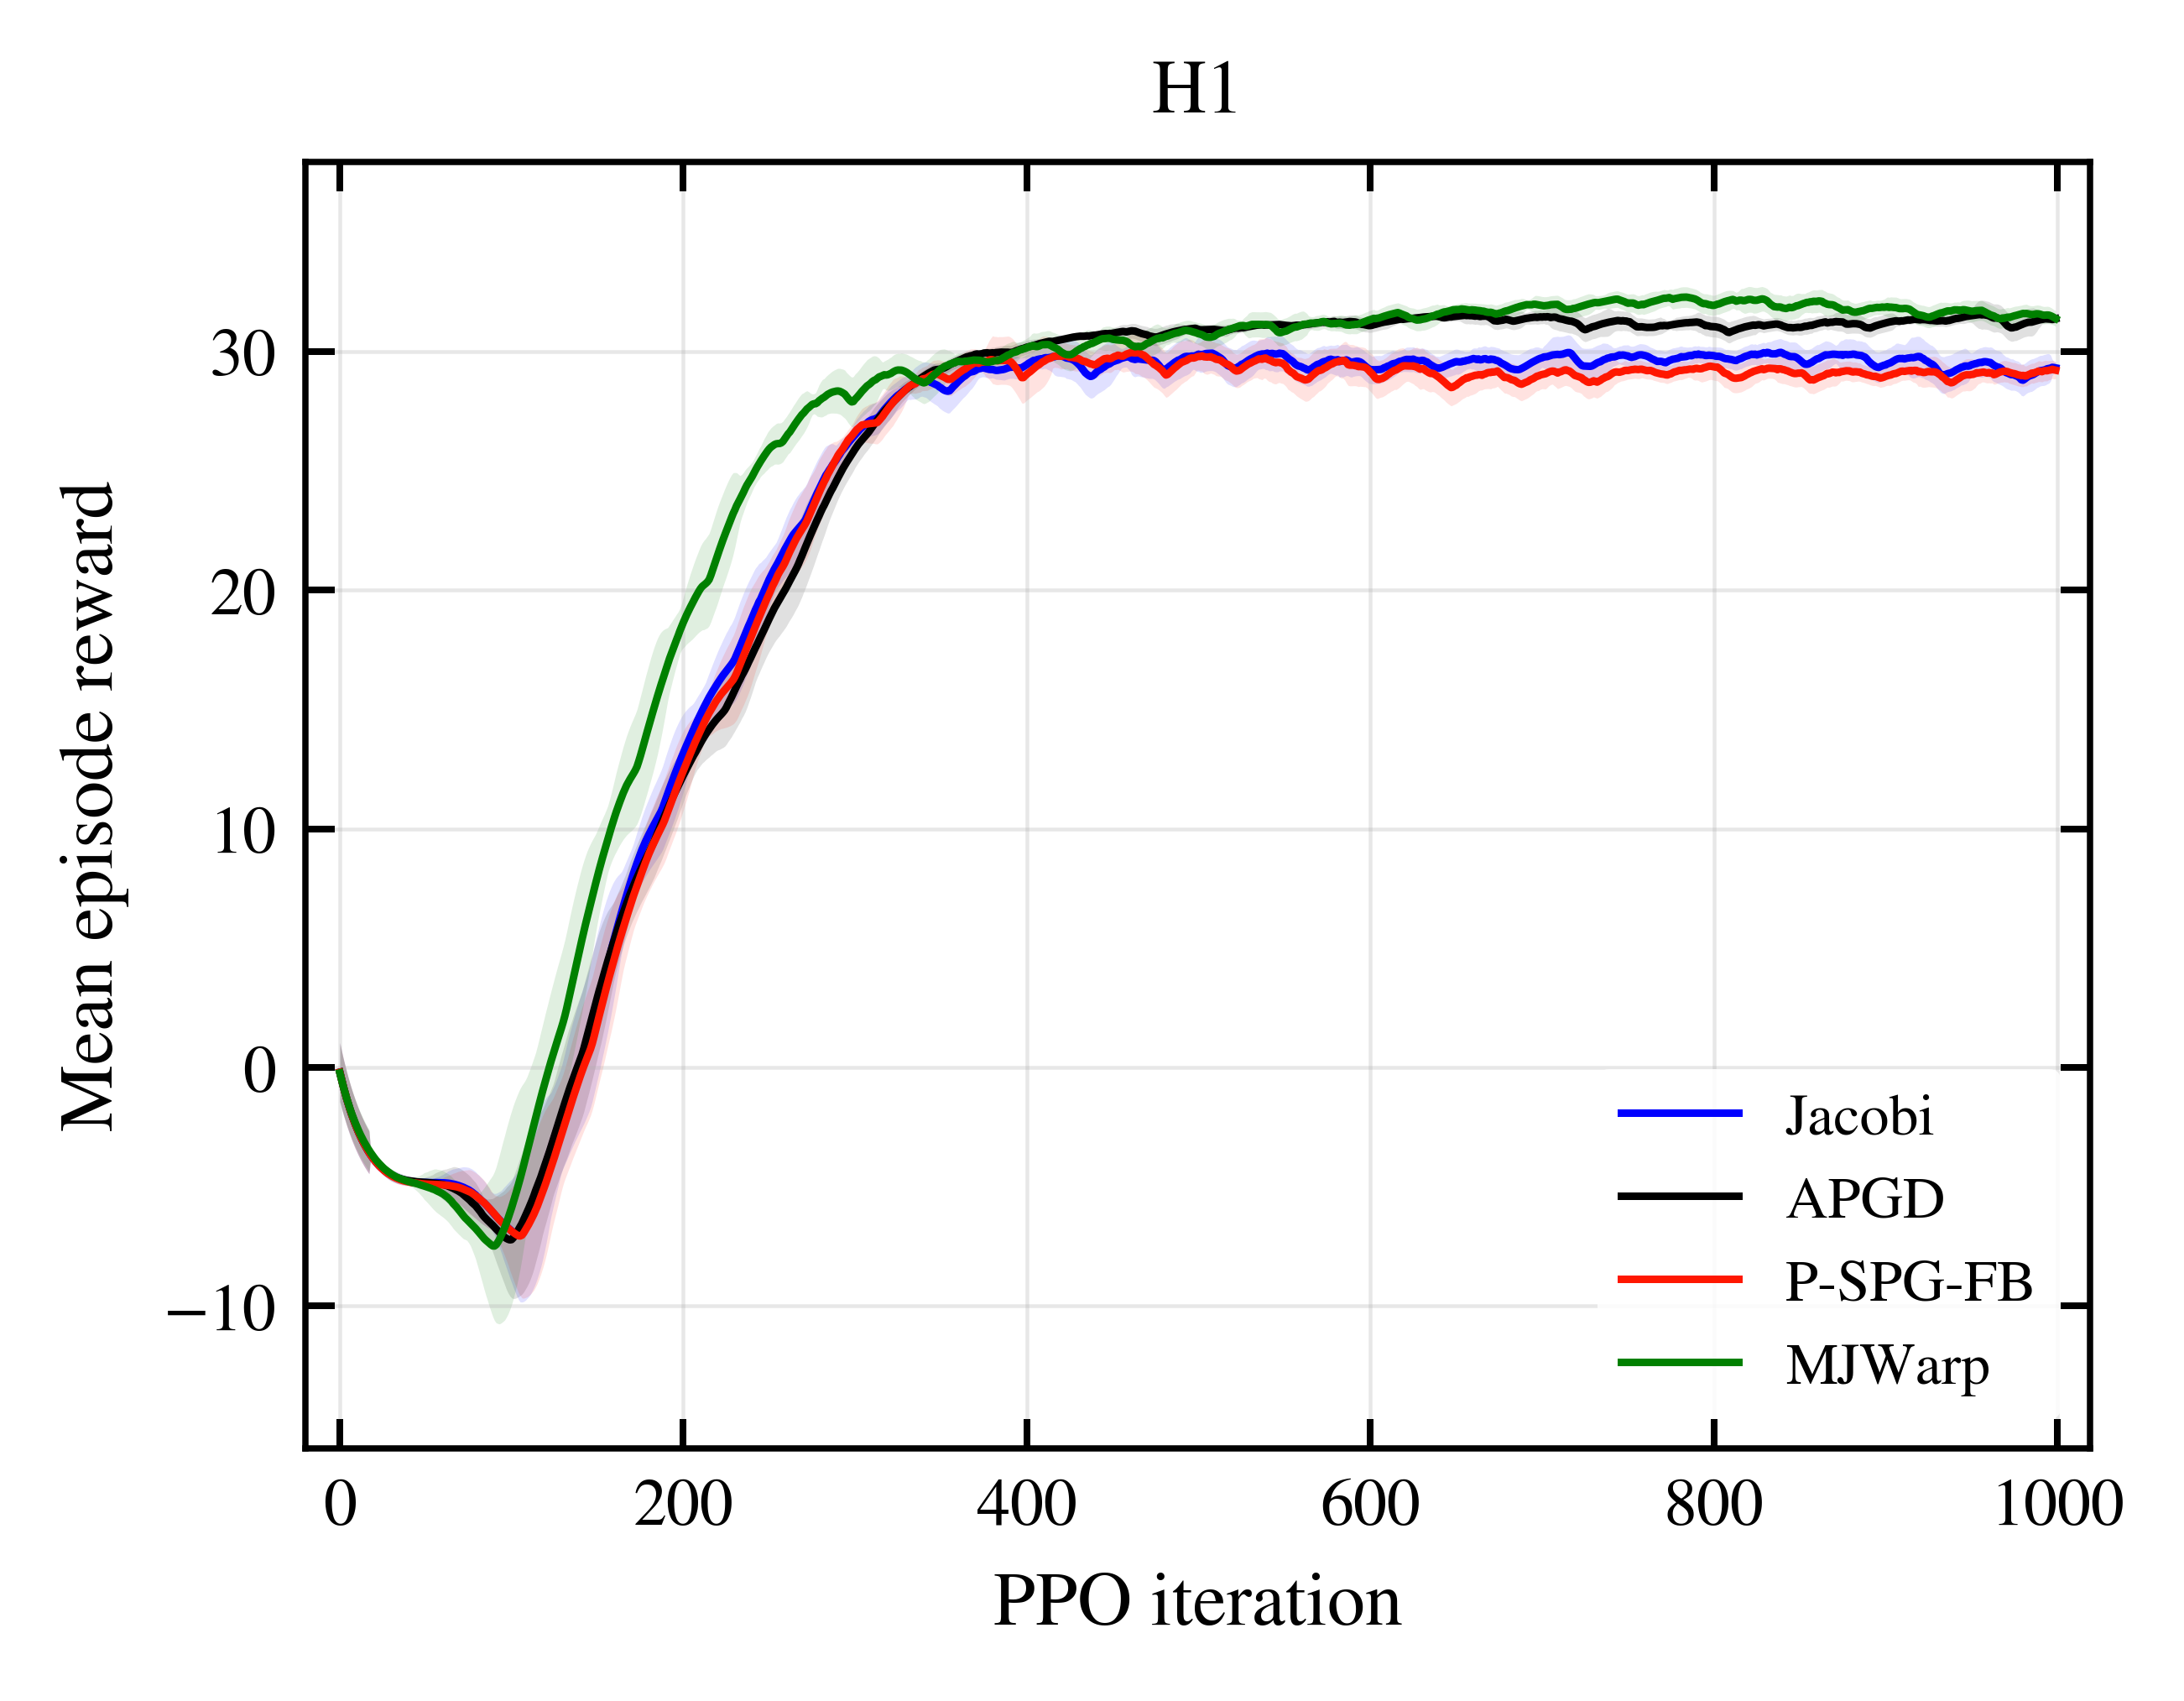
\includegraphics[width=\linewidth]{results/reinforcement_learning/figures/h1_jacobi_mjwarp_apgd_progress.png}
  \end{minipage}\hfill
  \begin{minipage}[t]{0.47\textwidth}
    \centering
    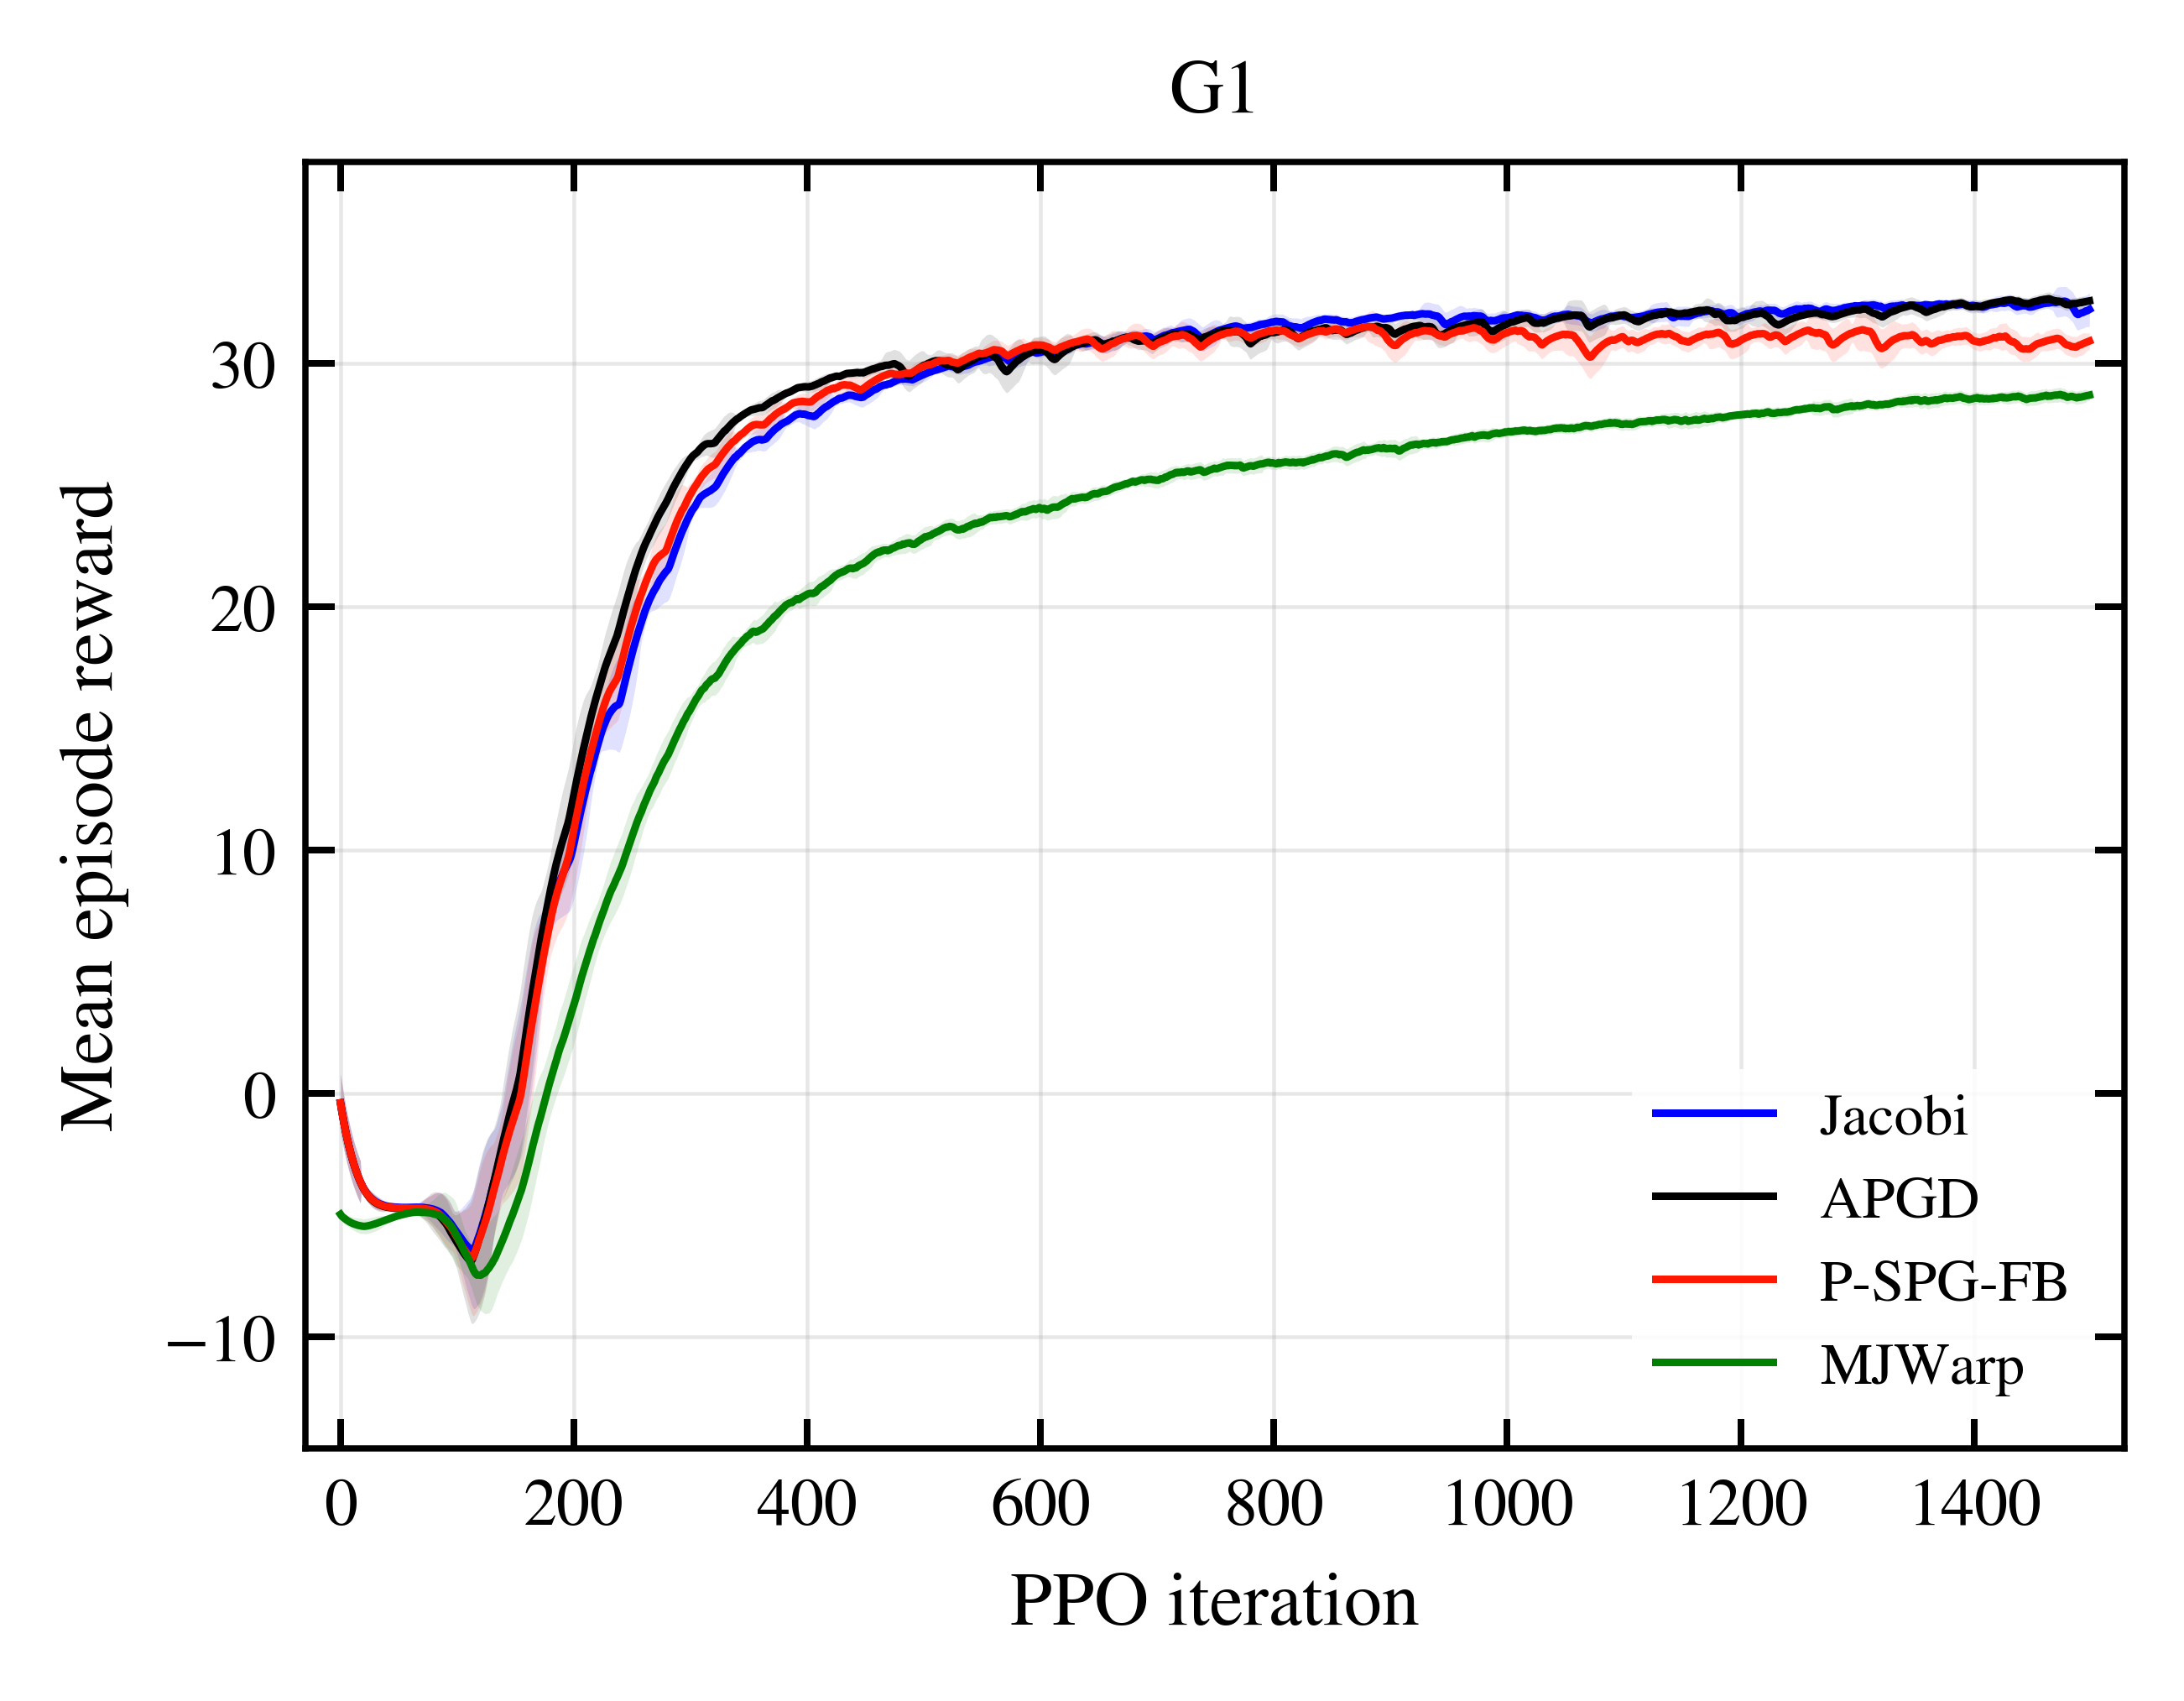
\includegraphics[width=\linewidth]{results/reinforcement_learning/figures/g1_jacobi_mjwarp_apgd_progress.png}
  \end{minipage}\\[4pt]
  \begin{minipage}[t]{0.47\textwidth}
    \centering
    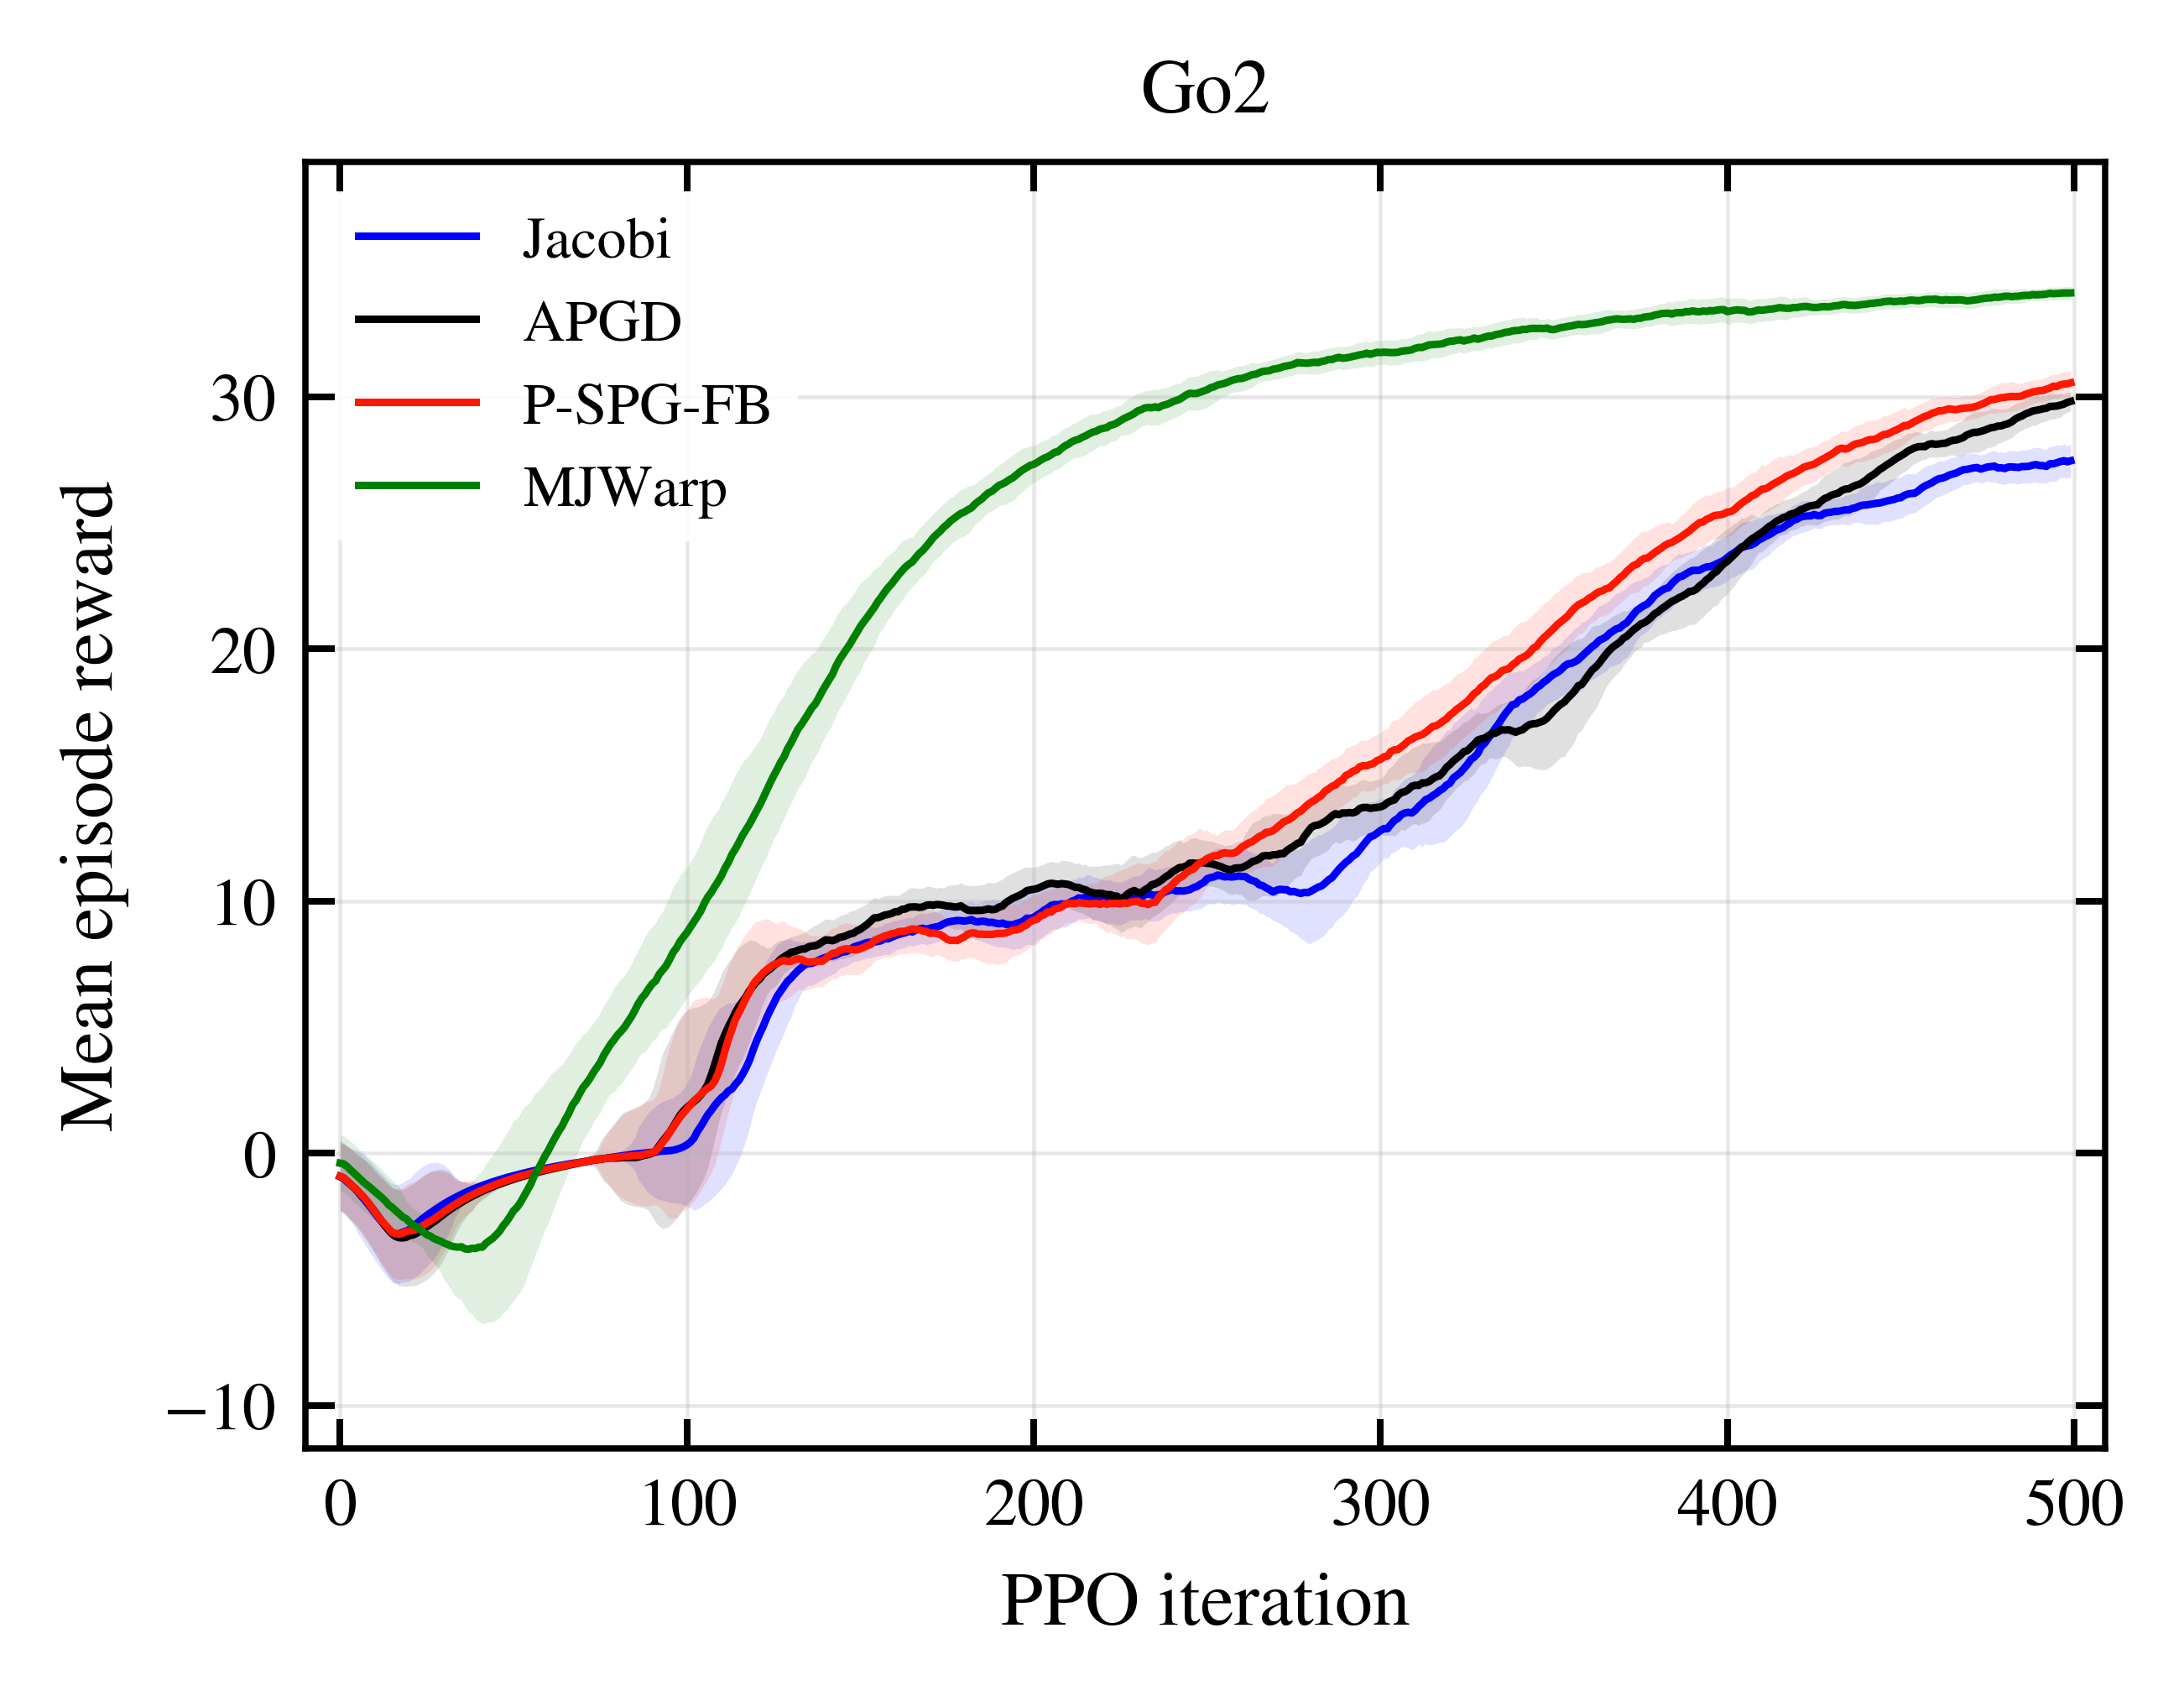
\includegraphics[width=\linewidth]{results/reinforcement_learning/figures/go2_jacobi_mjwarp_apgd_progress.png}
  \end{minipage}\hfill
  \begin{minipage}[t]{0.47\textwidth}
    \centering
    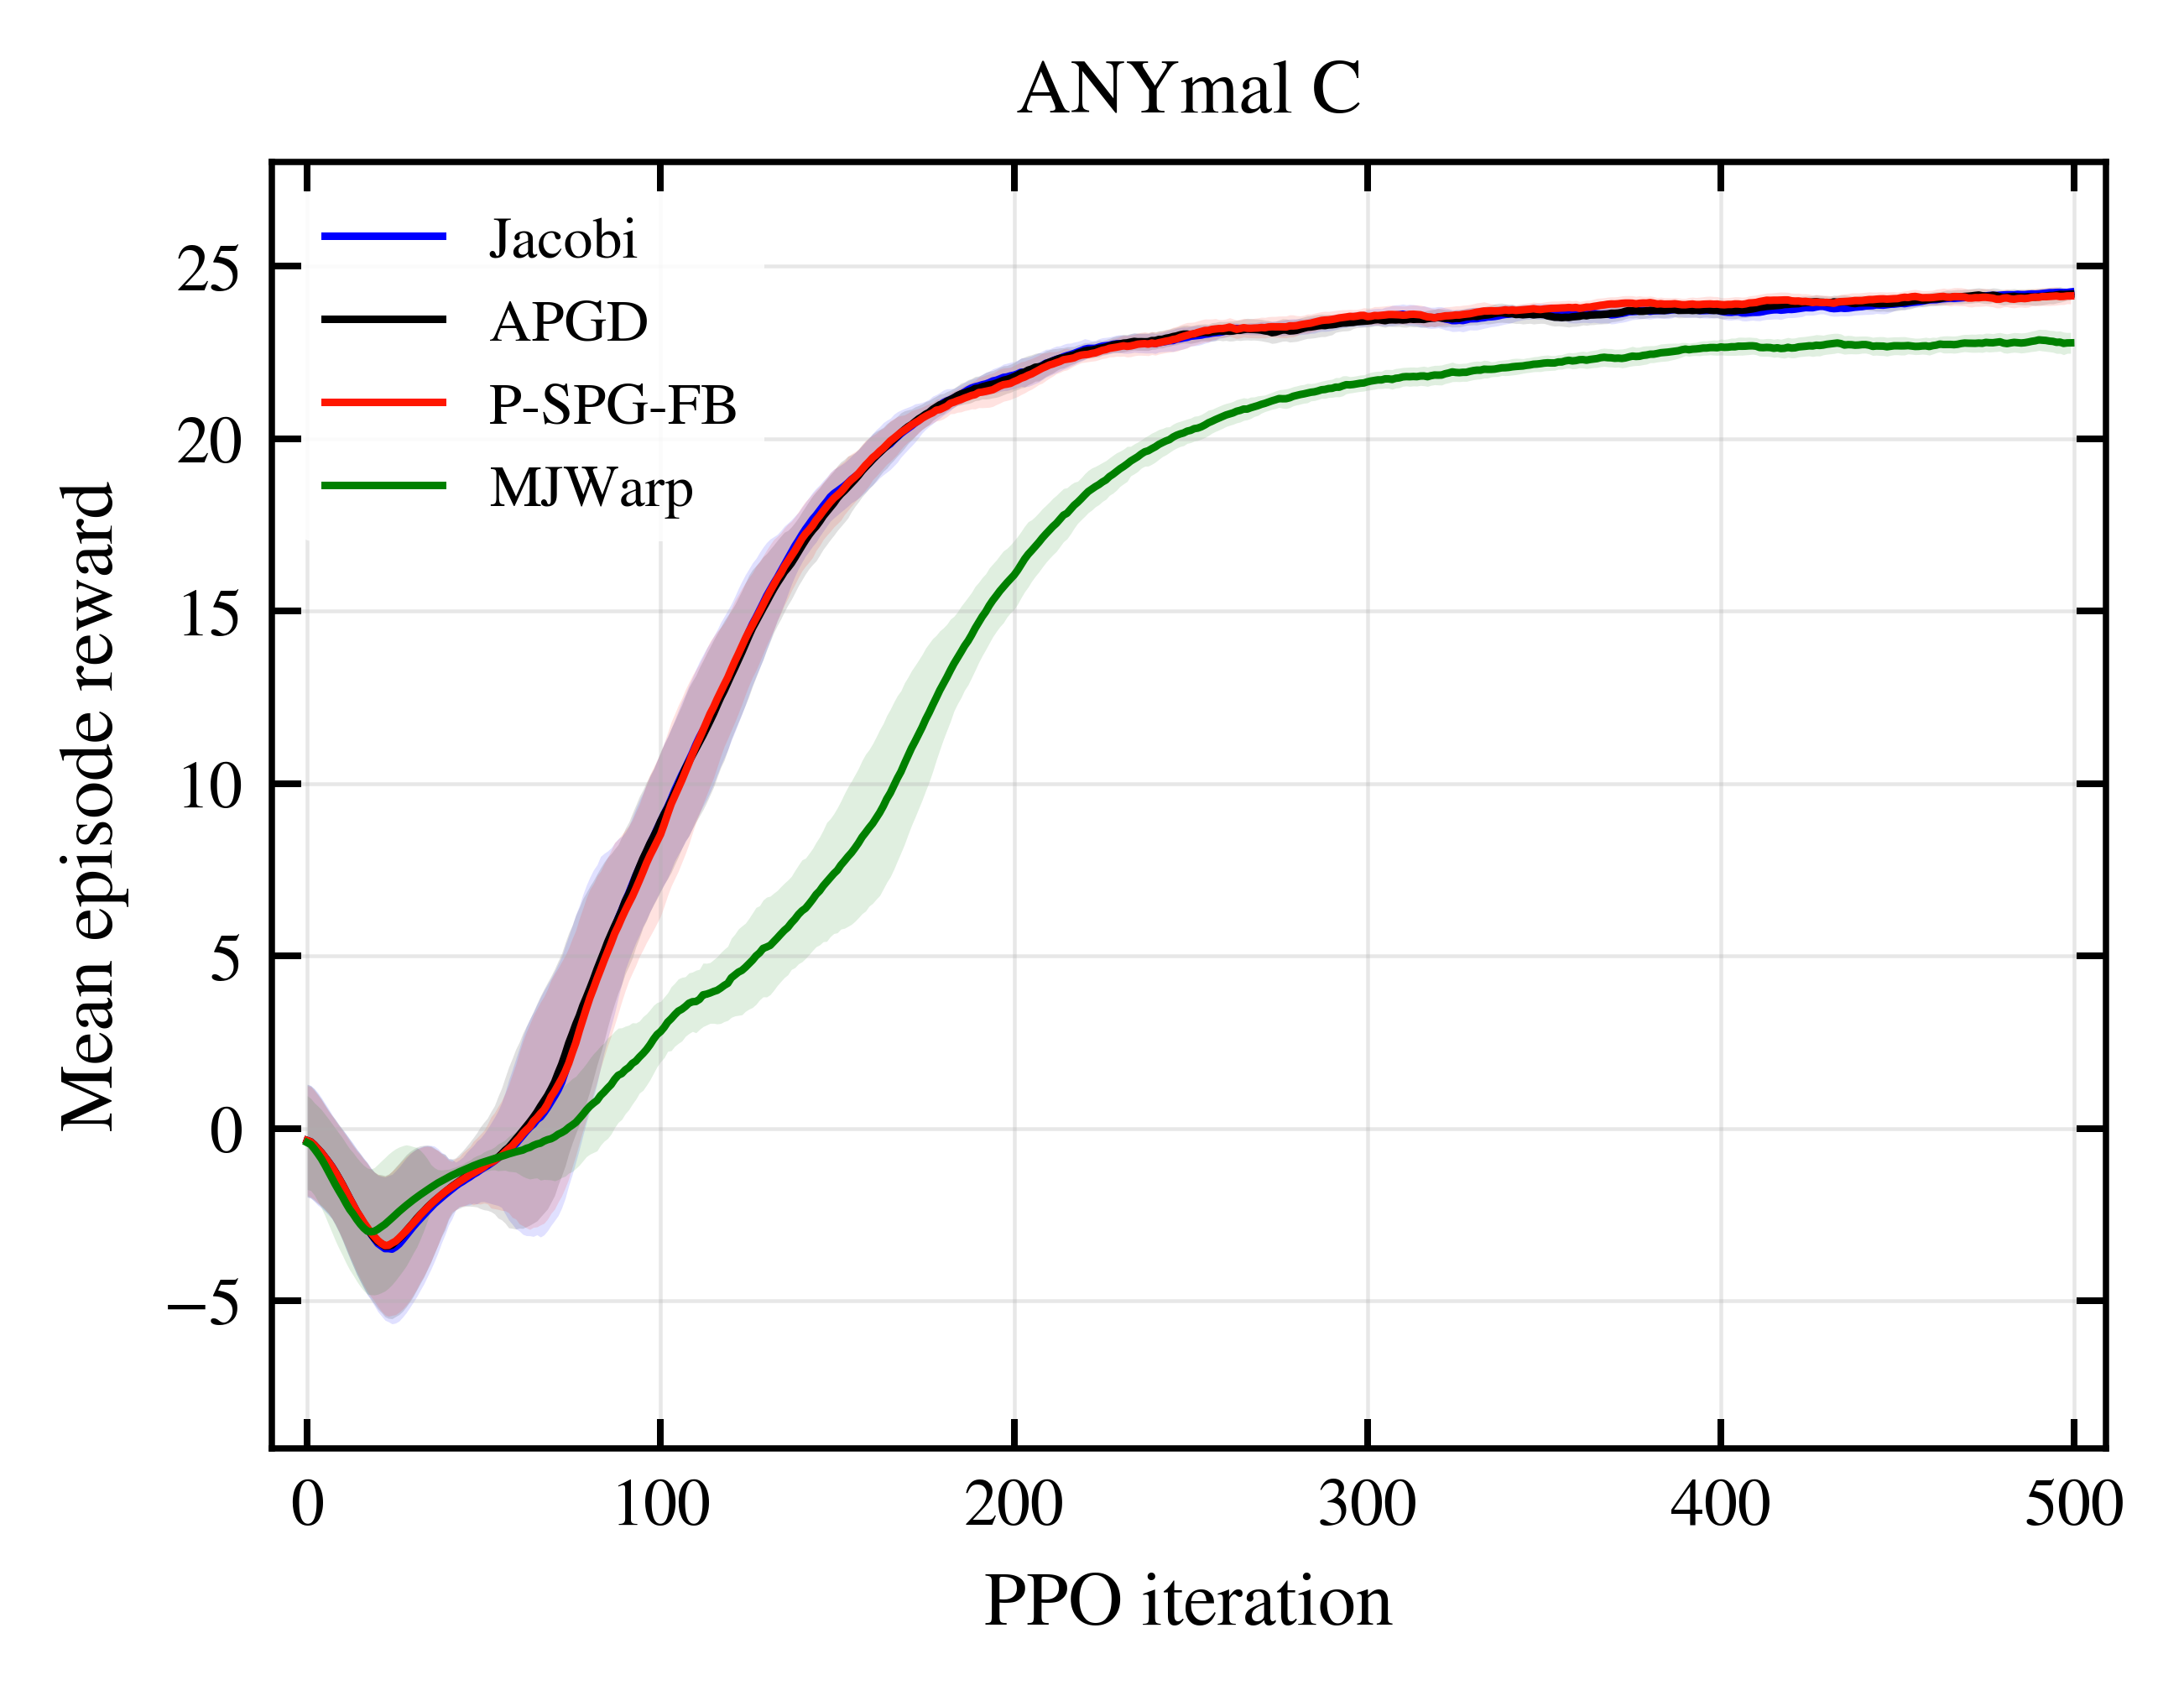
\includegraphics[width=\linewidth]{results/reinforcement_learning/figures/anymal_c_jacobi_mjwarp_apgd_progress.png}
  \end{minipage}
  \caption{Reinforcement-learning reward curves for six environments. Curves
  show EMA-smoothed reward with a rolling one-standard-deviation within-run
  variability band. Legends identify the solver; the Humanoid panel also
  reports median training throughput in frames per second.}
  \label{fig:rl-all-environments}
\end{figure*}

There is no consistent reward ordering across tasks. The SCC and MJWarp curves
finish near one another on H1; SCC Jacobi exceeds MJWarp in the displayed G1
and Anymal C runs, whereas MJWarp finishes higher on Ant and Go2. On Humanoid,
APGD finishes above MJWarp, P-SPG-FB reaches a comparable reward, and Jacobi
finishes slightly lower. All three SCC contact solvers support policy learning
under the selected configurations.

MJWarp has the highest median rollout throughput in all six panels. Within SCC,
Jacobi is consistently faster than APGD, which is faster than P-SPG-FB; this
ordering matches the increasing per-iteration work seen in the fixed-contact
benchmark. The magnitude of each gap depends on the environment and reflects
the complete native dynamics and collision paths. For Humanoid, the median
rates are 316, 176, 122, and 55 thousand frames per second for MJWarp,
Jacobi, APGD, and P-SPG-FB, respectively, as reported in the panel legend.

These six robots are tree structured, the regime in which reduced coordinates
can eliminate tree-joint constraints. SCC addresses the complementary modeling
requirement by representing closed constraint graphs with the same bilateral
rows used for ordinary joints. We evaluate this capability on DR Legs.
\FloatBarrier

\subsection{Experimental validation}
\label{sec:experimental-validation}

\subsubsection{Go2}
\label{sec:go2-sim2sim}

We first evaluate transfer across physics implementations by executing trained
Go2 velocity and bipedal policies in the Unitree MuJoCo-C model. Both
transfers use the same flat scene, actuator mapping, 50 Hz control rate, and
four 2.5-second command phases: forward-$x$, lateral-$y$, yaw, and combined
motion. Each policy completes the ten-second playback. The accompanying paired
videos use synchronized frames with MJWarp on the left and Newton--SCC on the
right. Both SCC policies retain the commanded locomotion behavior after
transfer to MuJoCo-C.

To test transfer to hardware, we deploy a rough-terrain locomotion policy
trained with Newton--SCC on a physical Unitree Go2. The robot traverses the test
terrain using the learned gait, providing direct simulation-to-real validation
of a policy trained with the SCC dynamics. \Cref{fig:go2-rough-terrain} shows
a Newton--SCC policy rollout over the corresponding procedurally generated
rough terrain.

\begin{figure}[t]
  \centering
  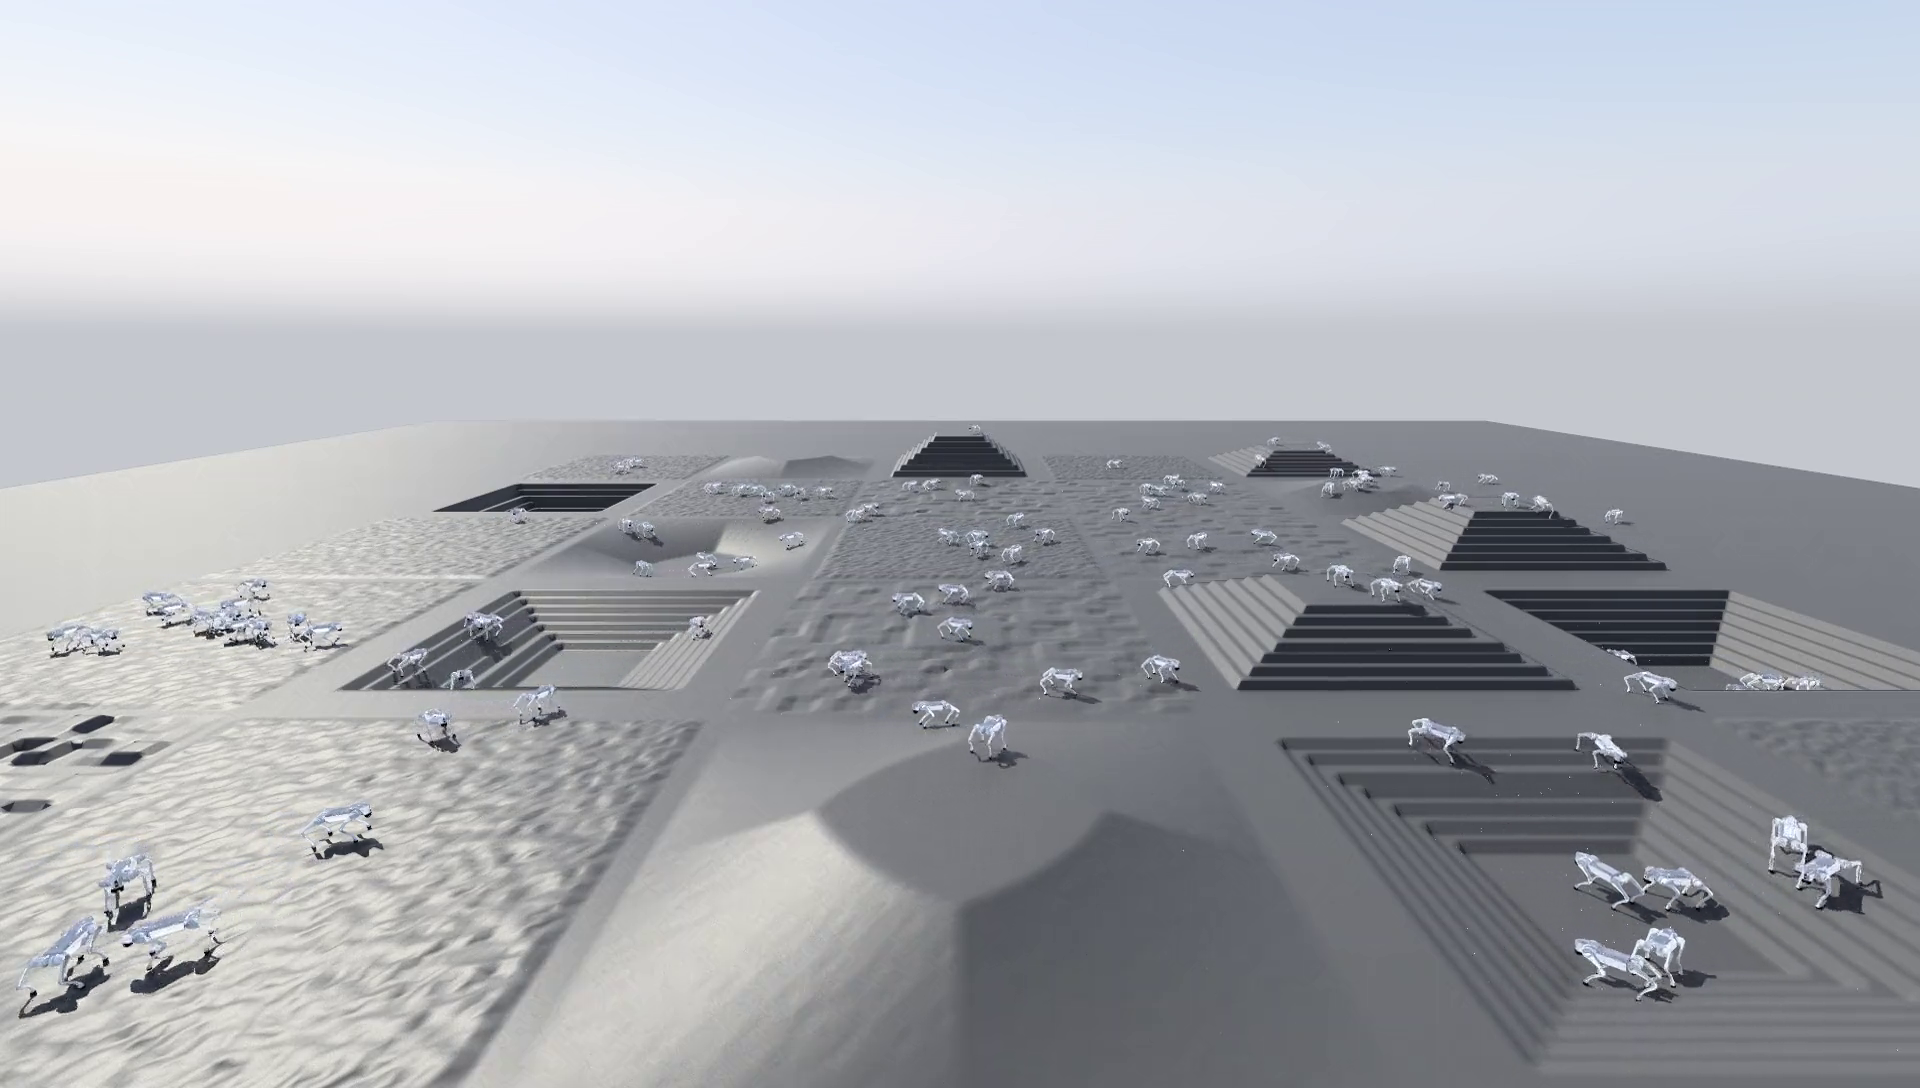
\includegraphics[width=0.82\linewidth]{results/reinforcement_learning/figures/go2_dvi_128env_rough_terrain_snapshot.png}
  \caption{Newton--SCC rough-terrain rollout for Unitree Go2.}
  \label{fig:go2-rough-terrain}
\end{figure}
\FloatBarrier

\subsubsection{G1}
\label{sec:g1-policy-transfer}

\subsubsection{BDX}
\label{sec:bdx-policy-transfer}

\subsubsection{Lanky Dog}
\label{sec:lanky-dog-policy-transfer}

\subsubsection{Dr Legs}
\label{sec:dr-legs-results}

DR Legs is a serial--parallel legged mechanism comprising 31 rigid bodies and
36 revolute joints, of which 12 are actuated. Its six independent kinematic
loops make policy learning an end-to-end test of bilateral closure, contact,
actuation, and control. The four knee loops are planar four-bar linkages. The
two ankle loops are spatial five-bar linkages whose closure has rank five,
leaving one physical hinge motion. This distinction is important for a
reduced-coordinate MuJoCo representation: a point-connect equality supplies
only three rows and leaves two spurious rotational degrees of freedom, whereas
two point-connect equalities supply six rows and are redundant. The native
MuJoCo equality set has no nonredundant five-row hinge-loop primitive. In the
maximal-coordinate SCC formulation, all revolute joints remain explicit
bilateral constraints, so the six loops require no spanning-tree reduction.

We compare SCC with one and two bilateral--unilateral sweeps and with Kamino
P-ADMM on the same locomotion task. All three runs use one physics substep per
$4\,\mathrm{ms}$ simulation step, seed 42, 4096 environments, and 1000 PPO
iterations. Both SCC runs use ten Jacobi contact iterations, cached bilateral
factorization, and no bilateral post-stabilization; they differ only in the
number of coupling sweeps. Kamino uses its P-ADMM solver configuration. For
this comparison, throughput is the median simulation rate over the final 500
PPO iterations.

\begin{figure}[!htbp]
  \centering
  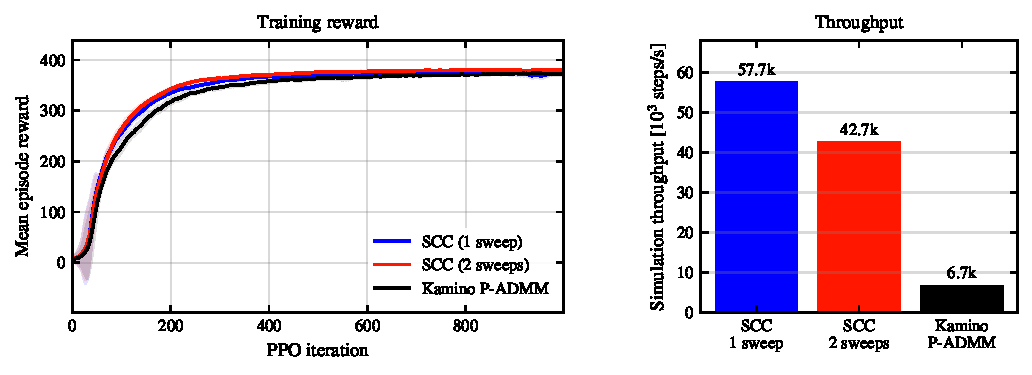
\includegraphics[width=0.99\linewidth]{results/reinforcement_learning/figures/drlegs_dvi_coupling_kamino_comparison.pdf}
  \caption{DR Legs policy learning with one and two SCC coupling sweeps and
  Kamino P-ADMM. \textbf{Left:} EMA-smoothed mean episode reward; shaded bands
  show the centered rolling within-run standard deviation. \textbf{Right:}
  simulation throughput.}
  \label{fig:dr-legs-comparison}
\end{figure}

All three configurations converge to comparable reward. SCC processes 57.7
thousand simulation steps per second with one sweep and 42.7 thousand with two
sweeps, compared with 6.7 thousand for Kamino P-ADMM. The one- and two-sweep
SCC configurations therefore achieve 8.58 and 6.35 times the throughput of
Kamino P-ADMM, respectively. The second sweep increases coupling between the
bilateral and unilateral solves at the cost of lower throughput.
\FloatBarrier

% =============================================================================
\section{Discussion}
\label{sec:discussion}

% =============================================================================
\section{Conclusion}
\label{sec:conclusion}

% =============================================================================
\appendix

\section{Joint Jacobian derivations}
\label{app:jacobians}
A holonomic constraint $C_i(\mathbf q)=0$ differentiates to the velocity form
$\mathbf d_i^{\top}\vv+\partial_t C_i=0$, contributing the row $\mathbf d_i^{\top}$
of $\Jac_b$. For the ball (spherical) joint, which forces two anchor points
$\mathbf x_a+\mathbf r_a$ and $\mathbf x_b+\mathbf r_b$ (world-frame lever arms
$\mathbf r_{\{a,b\}}$) to coincide, the per-body $3\times6$ blocks are
\begin{equation}
\Jac_{b,a}=\bigl[-\Id_3\ \big|\ \skewm{\mathbf r_a}\bigr],\qquad
\Jac_{b,b}=\bigl[+\Id_3\ \big|\ -\skewm{\mathbf r_b}\bigr],
\end{equation}
with $\skewm{\cdot}$ the cross-product matrix. A contact contributes, per
direction $\mathbf e\in\{\mathbf n_i,\mathbf t_{1,i},\mathbf t_{2,i}\}$,
\begin{equation}
\Jac_{u,a}=\bigl[-\mathbf e^{\top}\ \big|\ -(\mathbf s_{a}\times\mathbf e)^{\top}\bigr],\qquad
\Jac_{u,b}=\bigl[+\mathbf e^{\top}\ \big|\ +(\mathbf s_{b}\times\mathbf e)^{\top}\bigr],
\end{equation}
$\mathbf s_{\{a,b\}}$ the lever arms to the contact point. Other joints are row
subsets of the fixed joint (which removes all six relative DOF):

\begin{center}
\begin{tabular}{@{}lccc@{}}
\toprule
Joint & Position rows & Orientation rows & Total \\
\midrule
Fixed & 3 & 3 & 6 \\
Revolute & 3 & 2 & 5 \\
Prismatic & 2 & 3 & 5 \\
Ball (spherical) & 3 & 0 & 3 \\
Universal & 3 & 1 & 4 \\
\bottomrule
\end{tabular}
\end{center}

\section{Frictional contact as a cone complementarity problem}
\label{app:friction_ccp}
For contact $i$, write the contact-frame velocity $\uvel_i=(u_{n,i},\mathbf u_{T,i})$ and
impulse $\blam_i=(\lambda_{n,i},\boldsymbol\lambda_{T,i})$, with friction
coefficient $\mu_i$ and friction cone
$\cone_i=\{\|\boldsymbol\lambda_{T,i}\|\le\mu_i\lambda_{n,i}\}$.

\paragraph{Coulomb contact law.} An active contact must satisfy
\begin{align}
\text{(Signorini)}\ &\ 0\le u_{n,i}\ \perp\ \lambda_{n,i}\ge0, \label{eq:fr_sig}\\
\text{(friction cone)}\ &\ \|\boldsymbol\lambda_{T,i}\|\le\mu_i\lambda_{n,i},
  \label{eq:fr_cone}\\
\text{(max.\ dissipation)}\ &\ \boldsymbol\lambda_{T,i}
  =-\mu_i\lambda_{n,i}\,\frac{\mathbf u_{T,i}}{\|\mathbf u_{T,i}\|}
  \ \ \text{when sliding }(\mathbf u_{T,i}\neq\mathbf 0). \label{eq:fr_maxdiss}
\end{align}
The maximum-dissipation principle selects, among all impulses in the cone, the one
that opposes sliding and maximizes dissipated power.

\paragraph{Nonlinear coupling.} With the reduced map $\uvel=\Del\blam+\rhs$ of
\eqref{eq:ccp}, $\mathbf u_{T,i}$ is affine in the full impulse vector, while
\eqref{eq:fr_maxdiss} sets $\boldsymbol\lambda_{T,i}$ proportional to the product
of $\lambda_{n,i}$ and the sliding direction $\mathbf u_{T,i}/\|\mathbf u_{T,i}\|$
--- itself a function of $\blam$. This bilinear coupling makes the stacked system a
nonlinear complementarity problem (NCP) that is in general non-convex.

\paragraph{De Saxc\'e correction and the exact cone relation.} Introduce the modified
contact velocity that shifts the normal component by the sliding speed,
\begin{equation}
\bar{\uvel}_i=\uvel_i+\bigl(\mu_i\|\mathbf u_{T,i}\|,\,\mathbf 0\bigr),
\label{eq:desaxce}
\end{equation}
leaving the tangential part unchanged. Then \eqref{eq:fr_sig}--\eqref{eq:fr_maxdiss}
hold simultaneously iff the single cone complementarity
\begin{equation}
\cone_i\ni\blam_i\ \perp\ \bar{\uvel}_i\in\cone_i^{*},
\qquad \cone_i^{*}=\{\uvel:u_n\ge\mu_i\|\mathbf u_T\|\},
\label{eq:exact_ccp}
\end{equation}
is satisfied~\cite{desaxce1991}. Because the shift
$\mu_i\|\mathbf u_{T,i}\|$ depends on the unknown velocity, this is a nonlinear
cone-complementarity relation rather than the convex affine CCP solved below.

\paragraph{Anitescu--Tasora relaxation.} Dropping the De Saxc\'e shift
($\bar{\uvel}_i\mapsto\uvel_i$) gives the convex cone complementarity
\begin{equation}
\cone_i\ni\blam_i\ \perp\ \uvel_i\in\cone_i^{*},
\label{eq:at_ccp}
\end{equation}
which is the per-contact form of \eqref{eq:ccp} solved in this
paper~\cite{anitescu2006,tasora2011}. The relaxation produces artificial normal
velocity at sliding contacts because the dual-cone boundary requires a normal
component proportional to tangential slip. This effect vanishes at zero slip,
but it remains a modeling approximation in addition to time-discretization and
regularization errors.

\paragraph{Cone projection.}
\label{app:projection}
The projected solvers of \Cref{sec:solvers} enforce feasibility with the
Euclidean projection of $\blam=(\lambda_n,\boldsymbol\lambda_t)$ onto the
friction cone $\cone_i=\{\|\boldsymbol\lambda_t\|\le\mu_i\lambda_n\}$. The
projection has three cases:
\begin{equation}
\proj(\blam)=
\begin{cases}
\blam, & \|\boldsymbol\lambda_t\|\le\mu_i\lambda_n \quad\text{(inside the cone)},\\[4pt]
\mathbf 0, & \|\boldsymbol\lambda_t\|\le-\tfrac{1}{\mu_i}\lambda_n \quad\text{(inside the polar cone)},\\[4pt]
\dfrac{\lambda_n+\mu_i\|\boldsymbol\lambda_t\|}{1+\mu_i^2}
\begin{pmatrix}1\\[2pt]\mu_i\,\hat{\boldsymbol\lambda}_t\end{pmatrix},
& \text{otherwise (project to the boundary)},
\end{cases}
\label{eq:proj_app}
\end{equation}
with $\hat{\boldsymbol\lambda}_t=\boldsymbol\lambda_t/\|\boldsymbol\lambda_t\|$.
The cost is $O(1)$ per contact and the branch is a function of two scalar
comparisons.

\section{Determinism}
\label{app:determinism}
The scatter $\delta\vv_b=\sum_{c\in\mathcal C(b)}\M_b^{-1}\mathbf d_{c,b}\gamma_c$
accumulates contributions from every contact touching body $b$ concurrently.

\paragraph{Reduction order.} Floating-point addition is not associative:
$(a+b)+c$ and $a+(b+c)$ can differ in the last bit, because each intermediate sum
is rounded to the nearest representable float. When many threads add into the same
body with atomics, the summation order is fixed at run time by the hardware
schedule and varies between runs, so the reduction result varies by
$O(\varepsilon_{\mathrm{mach}})$. Near a cone boundary such a perturbation can flip
a projection branch and, over many steps, diverge the trajectory.

\paragraph{Fixed-point accumulation.}
Fixed-point integer accumulation removes dependence on the summation order,
provided no overflow occurs. Each real-valued contribution is quantized with a
common scale $S$:
\begin{equation}
\iota(x)=\operatorname{round}(S\,x)\in\mathbb Z,
\qquad
\delta\vv_b=\frac1S\sum_{c\in\mathcal C(b)}^{\ \mathbb Z}\ \iota\bigl(\M_b^{-1}\mathbf d_{c,b}\gamma_c\bigr),
\end{equation}
where the inner sum uses 64-bit atomic integer addition. The scale $S$ sets a
quantization interval of $1/S$ and is chosen to keep quantization error below
the solver tolerance while ensuring that every partial sum fits in 64 bits.
Subject to this range condition, the integer sum is independent of accumulation
order for a fixed quantization. Inner products that
drive control decisions (BB denominators, $r_{\mathrm{nat}}$, and descent tests)
use the same strategy, and fixed-bound loops can be predicated as described in
\Cref{sec:gpu}. These choices remove reduction-order variation in the solver;
they do not by themselves establish bitwise identity of every collision,
integration, and training operation in the end-to-end system.

% =============================================================================
\bibliographystyle{unsrtnat}
\bibliography{references}

\end{document}
